%%%%%%%%%%%%%%%%%%%%

\documentclass[graybox,envcountchap,sectrefs,deutsch]{svmono}

% choose options for [] as required from the list
% in the Reference Guide

\usepackage{mathptmx}
\usepackage{helvet}
\usepackage{courier}
\usepackage{type1cm}
\usepackage{braket}
\usepackage{qcircuit}

\usepackage{makeidx}         % allows index generation
\usepackage{graphicx}        % standard LaTeX graphics tool
                             % when including figure files
\usepackage{multicol}        % used for the two-column index
\usepackage[bottom]{footmisc}% places footnotes at page bottom

\usepackage{newtxtext}       % 
\usepackage{newtxmath}       % selects Times Roman as basic font

\usepackage{ngerman}


\usepackage{suffix}

\makeatletter
\newcommand{\chapterauthor}[1]{%
  {\parindent0pt\vspace*{-35pt}%
  \textsl{#1}%
  \par\nobreak\vspace*{35pt}}
  \@afterheading%
}
\makeatother


\usepackage[
    refsection=chapter,
    backend=biber,
    style=apa,
  ]{biblatex}
\addbibresource{references.bib} %Import the bibliography file



% see the list of further useful packages
% in the Reference Guide

\makeindex             % used for the subject index
                       % please use the style svind.ist with
                       % your makeindex program

%%%%%%%%%%%%%%%%%%%%%%%%%%%%%%%%%%%%%%%%%%%%%%%%%%%%%%%%%%%%%%%%%%%%%

\graphicspath{{./}{images/}}

\begin{document}

\author{Prof. Dr.-Ing. Rainer Neumann (Hrsg.)}
\title{Quantencomputer -- Ein aktueller Überblick}
\subtitle{Grundlagen, Hardware, Software, Anwendungen, Trends, Ethische Aspekte}
\maketitle

\frontmatter%%%%%%%%%%%%%%%%%%%%%%%%%%%%%%%%%%%%%%%%%%%%%%%%%%%%%%

%%\include{content/dedication}
%%\foreword


\vspace{\baselineskip}
\begin{flushright}\noindent
Karlsruhe, Juli 2025\hfill {\it Max Mustermann}\\
\end{flushright}



\preface

Die Quantenmechanik hat seit Beginn des 20. Jahrhunderts unser Verständnis der physikalischen Realität tiefgreifend verändert. Durch die Arbeiten von Wissenschaftlern wie Max Planck, Albert Einstein, Erwin Schrödinger und Werner Heisenberg wurde ein neues Fundament der Physik gelegt – eines, das klassische Konzepte von Kausalität und Determinismus in Frage stellte und den Weg für völlig neue Technologien ebnete.

Aus diesen Grundlagen entwickelte sich ab den 1970er Jahren ein neues Forschungsfeld: die Quanteninformationsverarbeitung. Erste theoretische Überlegungen zeigten, dass sich quantenmechanische Effekte nutzen lassen, um Informationen auf radikal neue Weise zu speichern, zu übertragen und zu verarbeiten. Diese Idee wurde in den 1990er Jahren durch die Entwicklung bedeutender Quantenalgorithmen konkretisiert – mit dem Versprechen, bestimmte Probleme deutlich effizienter zu lösen als klassische Computer es je könnten.

Heute stehen wir an einem technologischen Wendepunkt. Quantencomputer sind nicht mehr reine Theorie, sondern Realität: Mit sogenannten NISQ-Geräten (Noisy Intermediate-Scale Quantum) lassen sich bereits erste Anwendungen demonstrieren. Systeme auf Basis supraleitender Qubits, Ionenfallen oder photonischer Architekturen werden kontinuierlich weiterentwickelt. Neben großen Technologiekonzernen wie IBM, Google und Amazon sind auch Start-ups und universitäre Forschungsgruppen – auch in Deutschland – aktiv beteiligt. Parallel dazu entstehen staatlich geförderte Programme und eine globale Quantenökonomie.

Mit diesen Fortschritten jedoch treten neue gesellschaftliche Fragen in den Vordergrund. Die Aussicht auf massiv gesteigerte Rechenleistungen wirft sicherheitspolitische und ethische Herausforderungen auf. Wie können sensible Daten in Zukunft geschützt werden, wenn etablierte Verschlüsselungsverfahren durch Quantencomputer angreifbar werden? Sind Blockchain-basierte Systeme wie Kryptowährungen vor Manipulation sicher? Und wie lassen sich demokratische Infrastrukturen gegen hybride Bedrohungen und Cyberangriffe schützen?

Neben diesen praktischen Aspekten betreten wir auch philosophisches Neuland. Die wachsende Leistungsfähigkeit von Quantencomputern und künstlicher Intelligenz rückt die Frage in den Fokus, was menschliches Denken eigentlich ausmacht. Ist unser Bewusstsein bloß ein komplexer, deterministischer Prozess – simulierbar auf Maschinen? Oder liegt in der quantenmechanischen Unbestimmtheit möglicherweise ein Ursprung des freien Willens? Falls dem so ist, könnten Quantencomputer sogar eine Brücke zu neuartigen Formen maschinellen Lebens darstellen.

Dieses Buch widmet sich der faszinierenden Entwicklung von Quantencomputern und Quantentechnologien – von den physikalischen Grundlagen über den Stand der Technik bis hin zu zukünftigen Perspektiven. Es beleuchtet nicht nur die wissenschaftlich-technische Seite, sondern nimmt auch gesellschaftliche, ethische und sicherheitspolitische Implikationen in den Blick.

Entstanden ist dieses Buch im Rahmen eines Masterkurses mit dem Titel „What’s Next?“ an der Hochschule Karlsruhe. Es ist das Ergebnis eines didaktischen Experiments, bei dem sich eine Gruppe Studierender gemeinsam einem hochkomplexen Zukunftsthema nähert – mit dem Ziel, nicht nur Wissen zu erlangen und weiterzugeben, sondern auch zum kritischen Denken und Mitgestalten der technologischen Zukunft anzuregen.

\vspace{\baselineskip}
\begin{flushright}\noindent
Karlsruhe, Juli 2025\hfill {\it Rainer Neumann}\\
\end{flushright}

%%\include{content/acknowledgement}

\tableofcontents

%%\include{content/acronym}


\mainmatter%%%%%%%%%%%%%%%%%%%%%%%%%%%%%%%%%%%%%%%%%%%%%%%%%%%%%%%

\include{content/part1}
%\motto{Use the template \emph{chapter.tex} to style the various elements of your chapter content.}
\chapter{Physikalische Grundlagen}
\label{physics} % Always give a unique label

\chapterauthor{Karin Mustermann, Max Mustermann}

\abstract{some abstract}

\section{(Einführung in die Quantenmechanik für das Quantencomputing)}
\subsection{Motivation und Abgrenzung zur klassischen Physik }
\subsection{Wichtige Konzepte der Quantenmechanik }
\subsubsection{\textit{\textit{Zustände und Wellenfunktion} }}
\subsubsection{\textit{Observable und Messung}} 
\subsubsection{\textit{(Zeitentwicklung und Schrödingergleichung??)} }
\section{Zentrale Quantenphänomene }
\subsection{Superposition }
\subsection{Quanteninterferenz}
\subsection{Verschränkung }
\section{Quantenmessung }
\subsection{Grundlagen der Quantenmessung }
(projektive Messungen, Messoperatoren)
\subsection{Nichtdeterminismus}
(keine Vorhersagbarkeit, Vergleich mit klassischer Statistik, Rolle in Quantenalgorithmen) 
\subsection{Messprozess }
(Kollaps der Wellenfunktion, Einfluss auf das Quantensystem, Messung als irreversible Operation) 
\subsection{(((Technische Realisierung von Messungen, z.B. Fluoreszenz, Tunnelstrom, Photodetektion – eventuell aufgreifen in physikalische Realisierung (s. Supraleiter, Ionenfallen, etc.))) }
\section{Mathematische Beschreibung von Qubits }
\subsection{Hilbertraum und Zustandsvektoren }
\subsection{Bra-Ket-Notation }
\subsection{Bloch-Kugel-Darstellung }
\subsection{Zwei-Niveau-Systeme als Qubits (?) }
\section{Physikalische Realisierung von Qubits }
\subsection{Anforderungen an physikalische Systeme }
\subsubsection{Allgemeine Voraussetzungen}
(Kontrollierbarkeit, Isolation, Skalierbarkeit, Messbarkeit) 
\subsubsection{DiVincenzo Kriterien}
\subsubsection{Einführung in Dekohärenz / Fehlerquellen}
\subsection{Supraleitende Qubits }
\subsection{Ionenfallen-Qubits }
\subsection{Photonenbasierte Qubits}
\subsection{Spin-Qubits}
\subsection{Neutralatom-Qubits }



Zitat \cite{alhazmi_live_2024}

\cite{bergou_quantum_2021}

\printbibliography

%\motto{Use the template \emph{chapter.tex} to style the various elements of your chapter content.}


\chapter{Quantenhardware}
\label{hardware} % Always give a unique label
% use \chaptermark{}
% to alter or adjust the chapter heading in the running head

\chapterauthor{Dennis Hülsken, Jakob Krumke, Marc Meyer, Daniel Roth, Tom Slatosch}

\abstract{some abstract}

\section{Quantencomputer-Architekturen und Vernetzung}
Die Entwicklung leistungsfähiger Quantencomputer erfordert nicht nur fortschrittliche Qubit-Technologien, sondern ebenso durchdachte physikalische Architekturen und vernetzte Systeme. Dieses Kapitel bietet einen übergeordneten Einstieg in die technischen Grundlagen moderner Quantenhardware. Im Zentrum stehen der Aufbau skalierbarer Qubit-Arrays und die zugrundeliegenden Kopplungsmechanismen, die für kohärente Quantenoperationen essenziell sind.
\\\\
Abschließend gibt das Kapitel einen Ausblick auf erste Konzepte für ein Quanteninternet. Durch Quantenrouter, -repeater und Netzwerktopologien entsteht eine neue Form der verteilten Quantenverarbeitung, die weit über klassische Kommunikationsnetzwerke hinausgeht. Dieses Kapitel bildet damit die Grundlage für das Verständnis der nachfolgenden Plattformkapitel, die sich im Detail mit verschiedenen Qubit-Technologien und deren Implementierungen befassen.
\subsection{Aufbau eines Quantenprozessors: Qubit-Array, Kopplungsmechanismen}
Ein Quantenprozessor ist im Kern ein System, das aus vielen präzise steuerbaren Qubits besteht. Damit ein solcher Prozessor funktioniert, müssen die Qubits in einen definierten Anfangszustand gebracht werden können, es müssen grundlegende Rechenoperationen – sogenannte Quantengatter – an ihnen durchgeführt werden können, und ihre Zustände müssen am Ende ausgelesen werden können. (\cite{WasIstQuantencomputing}).
Es gibt verschiedene Technologien, um Qubits zu realisieren. Zwei der am weitesten entwickelten Ansätze sind supraleitende Qubits und Ionenfallen. Supraleitende Qubits nutzen den Josephson-Effekt, um nichtlineare Schwingkreise zu konstruieren, die quantisierte Energiezustände besitzen und bei extrem tiefen Temperaturen (weniger als 15 mK) betrieben werden. Ionenfallen hingegen fangen einzelne geladene Atome ein und nutzen deren elektronische Energiezustände als Qubits. (\cite{qtPrimaerQubitsBasisbausteineFuer2025}) Um eine größere Rechenleistung zu erzielen, werden diese Qubits oft in Qubit-Arrays angeordnet, um eine Vielzahl von ihnen miteinander zu verbinden und komplexere Berechnungen zu ermöglichen.
Die Interaktion und Steuerung der Qubits erfordert präzise Kopplungsmechanismen. Bei supraleitenden Qubits werden Mikrowellenimpulse eingesetzt, während bei Ionenfallen Laserstrahlen zum Einsatz kommen, um Übergänge zwischen den Energiezuständen der Qubits gezielt anzuregen und so Rechenoperationen durchzuführen. (\cite{boterSpiderwebArraySparse2022}) Diese Steuermechanismen sind entscheidend für die Ausführung von Quantengattern und die Manipulation der Qubit-Zustände. Die Leistung eines Quantencomputers hängt also nicht nur von der Qualität der physikalischen Qubits ab, sondern ebenso von der Präzision und Geschwindigkeit der klassischen Steuerungselektronik und Messsysteme. Die gesamte Architektur eines Quantencomputers ist ein komplexes, mehrschichtiges System, in dem klassische und quantenmechanische Komponenten perfekt synchronisiert zusammenarbeiten müssen. (\cite{WasIstQuantencomputing}).
Eine der größten Herausforderungen beim Bau von Quantenprozessoren ist die extreme Anfälligkeit der Qubits. Schon minimale Störungen aus der Umgebung, wie Strahlung, Temperaturschwankungen oder Materialdefekte, können dazu führen, dass die Qubits ihren empfindlichen Quantenzustand verlieren – ein Phänomen, das als Dekohärenz bezeichnet wird. (\cite{WasIstQuantencomputing}). Diese Dekohärenz führt unweigerlich zu Fehlern bei den Berechnungen. Um diesen Fehlern entgegenzuwirken, ist eine hochentwickelte Fehlerkorrektur unerlässlich. Oft müssen Dutzende oder sogar Hunderte von physikalischen Qubits kombiniert werden, um ein einziges, stabiles "logisches Qubit" zu bilden, das vor externen Einflüssen geschützt ist. Die extreme Empfindlichkeit der Qubits ist somit die größte technische Hürde, die nicht nur aufwendige Kühlung und Abschirmung erfordert, sondern auch eine enorme Redundanz in Form vieler physikalischer Qubits für ein einziges zuverlässiges logisches Qubit. (\cite{QuantencomputerWikipedia}) Dies verdeutlicht, dass die Entwicklung von Quantencomputern eine ebenso große ingenieurtechnische und materialwissenschaftliche Herausforderung ist wie eine rein physikalische. (\cite{wissenschaftenMitSupraleitendenQubits2021})
\subsection{Konzepte des Quanteninternets, Quantenrepeater, Quantenrouter, Verschränkungsverteilung}
Das Quanteninternet ist eine aufstrebende Technologie, die das Potenzial hat, die Art und Weise, wie Daten übertragen und gespeichert werden, grundlegend zu verändern. Im Gegensatz zu herkömmlichen Netzwerken, die Informationen in klassischen Bits übertragen, nutzt das Quanteninternet Qubits und deren quantenmechanische Eigenschaften wie Superposition und Verschränkung, was die Übertragungseffizienz erheblich steigern kann. (\cite{WasIstQuantencomputing})
Ein entscheidender Vorteil des Quanteninternets liegt in seiner Sicherheit. Quantenkommunikation basiert auf Quantenkryptografie, die durch die physikalischen Gesetze der Quantenmechanik, insbesondere die Nicht-Klonbarkeit von Qubits, ein nahezu perfektes Maß an Sicherheit bietet. Abhörversuche würden sofort erkannt, da jede Messung oder Manipulation eines Qubits dessen empfindlichen Zustand kollabieren lässt. Diese physikalisch bedingte, praktisch unknackbare Sicherheit ist ein großer Unterschied zu klassischen Verschlüsselungsmethoden, die auf mathematischen Annahmen basieren und potenziell durch zukünftige Quantencomputer geknackt werden könnten.4 Die Sicherheit ist somit der primäre und überzeugendste Treiber für die Entwicklung von Quantennetzwerken. (\cite{QuanteninternetZukunftTechnologie})
Neben der Sicherheit verspricht das Quanteninternet auch eine potenziell höhere Geschwindigkeit der Datenübertragung. Dank der Quantenverschränkung können Informationen instantan ausgetauscht werden, unabhängig von der geografischen Entfernung der miteinander verschränkten Qubits. Trotz dieses enormen Potenzials stehen der globalen Umsetzung noch viele technische Hürden im Weg, insbesondere die Aufrechterhaltung der Kohärenz der Qubits über große Distanzen und die Skalierbarkeit des gesamten Netzwerks.
Um die Übertragung über große Entfernungen zu ermöglichen und die Probleme der Dekohärenz zu überwinden, sind spezielle Quantenrepeater erforderlich.  (\cite{AuswirkungenQuanteninternetsAuf2025}) Diese Repeater sind keine einfachen Signalverstärker wie im klassischen Internet, die ein Signal kopieren und verstärken würden – was bei Quanteninformationen aufgrund des No-Cloning-Theorems unmöglich ist. Stattdessen sind es komplexe Quantengeräte, die Quantenzustände über das Prinzip des "Entanglement Swapping" (Verschränkungstausch) über weite Strecken übertragen, ohne die wertvolle Quanteninformation zu zerstören.Dies macht sie zu einem kritischen technologischen Baustein für den Aufbau eines wirklich globalen Quanteninternets, da die direkte Übertragung fragiler Quantenzustände über lange Glasfaserkabel derzeit aufgrund von Verlusten und Dekohärenz nicht praktikabel ist. (\cite{QuanteninternetZukunftTechnologie})
Die Vision des Quanteninternets beinhaltet nicht nur lokale Netzwerke, sondern auch die Vernetzung separater Quantenprozessor-Module über Quantenkanäle. Dies deutet auf eine modulare und verteilte Architektur hin, bei der Recheneinheiten nicht in einem einzigen riesigen System gebündelt sind, sondern mehrere kleinere Module ein hochleistungsfähiges Netzwerk bilden können.(\cite{QuanteninternetRucktGreifbare}) Für die physikalische Infrastruktur sind spezielle Glasfaserkabel und Quantenrouter erforderlich, um die Quantenverschränkung und -übertragung zu gewährleisten. Diese Quantenrouter würden dabei helfen, die verschränkten Photonen oder Qubits zu ihren Zielen zu leiten.(\cite{AuswirkungenQuanteninternetsAuf2025})Die Verteilung von Verschränkung ist der Kern des Quanteninternets; es geht darum, verschränkte Qubit-Paare zwischen verschiedenen Knotenpunkten im Netzwerk zu etablieren und zu erhalten. Dies dient dann als Ressource für sichere Kommunikation oder für verteilte Quantenberechnungen.
Da der Aufbau eines globalen Quanteninternets noch in weiter Ferne liegt, werden hybride Netzwerklösungen diskutiert. Diese könnten klassische und quantenbasierte Datenübertragung kombinieren, um eine nahtlose Integration zu ermöglichen und einen Übergang zu schaffen. (\cite{QuanteninternetZukunftTechnologie}) Erste Feldexperimente zeigen bereits, dass die Verteilung von verschränkten Photonen über kommerziell genutzte Glasfasern parallel zum klassischen Datenverkehr möglich ist, was die Kompatibilität bestehender Infrastrukturen unterstreicht.

\section{Einführung in Quantenhardwareplattformen}
Die physikalische Realisierung eines Quantencomputers ist maßgeblich durch die Wahl der zugrunde liegenden Hardwareplattform bestimmt. Quantenhardware bildet das technische Fundament für alle quantenlogischen Operationen und beeinflusst entscheidend die Skalierbarkeit, Robustheit und Anwendungsdomänen heutiger und zukünftiger Quantencomputer. Der Begriff „Plattform“ bezeichnet hierbei die physikalischen Systeme, mit denen Qubits realisiert, kontrolliert und gemessen werden. Zwei übergeordnete Klassen haben sich als besonders relevant herausgestellt: Festkörperbasierte und atomare Plattformen (\cite{schmaltzQuantentechnologienUndQuantenOkosysteme2025, homeisterQuantumComputingVerstehen2015}.

\subsection{Überblick über Plattformtypen}
\begin{itemize}
\item \textbf{Festkörperplattformen} nutzen mikroskopische Strukturen in festen Materialien – typischerweise Halbleiter oder supraleitende Metalle, um Qubits durch elektrische, magnetische oder optische Eigenschaften zu realisieren. Bekannte Beispiele sind supraleitende Transmon-Qubits, Quantenpunkte und diamantbasierte NV-Zentren.
\item \textbf{Atomare Plattformen} beruhen auf der Manipulation einzelner Atome oder Ionen, die mithilfe elektromagnetischer Felder in Fallen gespeichert und durch Laser- oder Mikrowellenpulse angeregt werden. Dazu zählen Ionenfallen, Neutralatomfallen und photonische Systeme.
\end{itemize}

Diese Plattformen unterscheiden sich signifikant hinsichtlich ihrer technologischen Reife, Kohärenzeigenschaften und praktischen Einsatzmöglichkeiten. Tabelle \ref{tab:plattformvergleich} stellt zentrale Merkmale beider Klassen gegenüber:

\begin{table}[h]
\centering
\caption{Vergleich atomarer und festkörperbasierter Quantenhardwareplattformen}
\label{tab:plattformvergleich}
\begin{tabular}{|p{4cm}|p{5cm}|p{5cm}|}
\hline
\textbf{Aspekt} & \textbf{Atomare Plattformen} & \textbf{Festkörperplattformen} \\
\hline
Beispiele & Ionenfallen, Rydberg-Atome & Transmon-Qubits, NV-Zentren, Quantenpunkte \\
Qubit-Implementierung & Einzelatome oder Ionen in Fallen & Elektronen-/Spinzustände in Materialien \\
Kohärenzzeiten & Sehr lang (bis zu Minuten) & Kürzer (µs–ms) \\
Steuerung & Laser- und Mikrowellenfelder & Elektrische/optische Signale, Mikrowellen \\
Herstellung & Komplexe atomare Präparation & Standardisierte Halbleiterfertigung \\
Skalierbarkeit & Eingeschränkt durch optische Systeme & Gute Integrationsmöglichkeiten \\
Anwendungen & Metrologie, Quantensimulation & Algorithmische Anwendungen, Optimierung \\
\hline
\end{tabular}
\end{table}


\subsection{Technologischer Reifegrad und Herausforderungen}
Laut der „Schwerpunktstudie Quantenökosysteme“ des Fraunhofer ISI befinden sich supraleitende Systeme (v.a. Transmon-Qubits) sowie Ionenfallen derzeit auf dem höchsten technologischen Entwicklungsstand. Beide Plattformen konnten bereits fehlerkorrigierte Gatter demonstrieren, wenngleich unter hohem technologischem Aufwand (\cite{schmaltzQuantentechnologienUndQuantenOkosysteme2025}).
\\
Andere Ansätze wie photonische Qubits oder NV-Zentren bieten teils attraktive Eigenschaften (z.B. Raumtemperaturbetrieb oder geringe Dekohärenzanfälligkeit), sind jedoch noch mit praktischen Limitierungen bei Skalierung, Adressierbarkeit oder Gatterqualität konfrontiert (\cite{homeisterQuantumComputingVerstehen2015}).
\\
Die derzeit gängigen Quantencomputer zählen zur Klasse der sogenannten \textit{Noisy Intermediate-Scale Quantum}-Systeme (NISQ). Diese verfügen über 50–150 Qubits, erlauben jedoch keine vollumfängliche Fehlerkorrektur. Anwendungen beschränken sich auf experimentelle Algorithmen mit begrenzter Komplexität (\cite{schmaltzQuantentechnologienUndQuantenOkosysteme2025, homeisterQuantumComputingVerstehen2015}).
\\
Ein Durchbruch in Richtung großskaliger, universeller Quantencomputer wird eine massive Erhöhung der Qubit-Zahl, Schätzungen gehen von $10^5$ bis $10^6$ Qubits aus, sowie Fortschritte bei Fehlertoleranz und Architektur erfordern (\cite{schmaltzQuantentechnologienUndQuantenOkosysteme2025}).

\subsection{Ausblick auf die Kapitelstruktur}
Die folgende Gliederung dieses Teils orientiert sich an den bedeutendsten physikalischen Plattformen des aktuellen Forschungsstandes. Jede Plattform wird hinsichtlich ihrer physikalischen Grundlagen, technischer Implementierung, Herausforderungen und Perspektiven systematisch analysiert. Die Kapitel im Überblick:

\begin{itemize}
\item \textbf{Kapitel 1.3: Supraleitende Qubits}
\item \textbf{Kapitel 1.4: Ionenfallen-Qubits}
\item \textbf{Kapitel 1.5: Diamantbasierte Qubits (NV-Zentren)}
\item \textbf{Kapitel 1.6: Weitere Plattformen}
\item \textbf{Kapitel 1.7: Vergleichende Bewertung der Quantenhardware-Architekturen} 
\item \textbf{Kapitel 1.8: Praxisbeispiel am IBM Q}
\end{itemize}

Dieses Einführungskapitel legt somit den Grundstein für ein vertieftes Verständnis der komplexen und heterogenen Hardwarelandschaft im Quantencomputing. Es zeigt, dass die Wahl der Plattform nicht nur technische, sondern auch strategische Bedeutung für den weiteren Fortschritt in Forschung und Anwendung besitzt.

\section{Supraleitende Qubits}
Supraleitende Quantencomputer nutzen die Prinzipien der Quantenmechanik und die einzigartigen Eigenschaften von Supraleitern, um Quantenberechnungen durchzuführen. Diese Systeme sind darauf ausgelegt, komplexe Aufgaben in Bereichen wie Quantenchemie, Simulation, Kryptographie und Optimierung zu bewältigen, was ihnen potenzielle Vorteile gegenüber klassischen Systemen verschafft. Die Realisierung dieser Rechenvorteile hängt jedoch von der effizienten und skalierbaren Ausführung von Quantenprogrammen auf robuster Hardware ab, die für Quantenoperationen konzipiert ist.
\subsection{Implementierung von Quantenlogik}
\subsubsection{Grundlegende Prinzipien und Typen}
Die fundamentalen Einheiten der Quanteninformation in supraleitenden Systemen sind supraleitende Qubits, die als künstliche Atome mit quantisierten Energieniveaus fungieren. Diese Qubits werden typischerweise aus supraleitenden Schaltkreisen gefertigt, die Materialien wie Aluminium oder Niob verwenden und bei extrem niedrigen Temperaturen, nahe dem absoluten Nullpunkt (ca. 15 Millikelvin), betrieben werden (\cite{noauthor_ultimate_nodate}). Die Supraleitung, die bei diesen Temperaturen erreicht wird, gewährleistet einen widerstandslosen Stromfluss, was für die Aufrechterhaltung der Kohärenz der Qubits und ihrer Quantenzustände unerlässlich ist.
\\\\
Ein supraleitendes Qubit besteht häufig aus einem Induktor und einem Kondensator (LC-Oszillator), die durch einen Josephson-Kontakt verbunden sind. Der Josephson-Kontakt ist ein entscheidendes nichtlineares Element, das eine Anharmonizität in das Energiespektrum des Schaltkreises einführt. Diese Anharmonizität ist von größter Bedeutung, da sie sicherstellt, dass nur die beiden niedrigsten Energiezustände - der Grundzustand 0 and der erste angeregte Zustand 1 - als Qubit-Zustände dienen. Ohne diese Nichtlinearität würde der Quanten-LC-Schaltkreis als einfacher harmonischer Oszillator mit äquidistanten Energieniveaus fungieren, wodurch eine isolierte Zwei-Niveau-System-Nutzung als Qubit unmöglich wäre. Die präzise technische Gestaltung des Josephson-Kontakts und die Auswahl des supraleitenden Materials sind daher nicht nur Fertigungsdetails, sondern grundlegend für die Schaffung eines stabilen und adressierbaren Zwei-Niveau-Systems. Sie bestimmen die grundlegenden Eigenschaften des Qubits wie Anharmonizität, Kohärenzzeit und Rauschresistenz, die für zuverlässige Quantenoperationen unerlässlich sind. Die Betriebsumgebung von supraleitenden Quantencomputern erfordert extrem niedrige Temperaturen, typischerweise im Bereich von 10 bis 20 Millikelvin(mK). Um diese Temperaturen zu erreichen, werden komplexe Kühlsysteme, meist Dilution Refridgerators, benötigt. Um eine solch extreme Kühlung zu ermöglichen, wird die Phasenmischung von Helium-3 und Helium-4 verwendet. Eine genauere Beschreibung zum Aufbau der Kühlsysteme und deren Funktionsweise sowie aktuelle Modelle, sind im Kapitel 1.2.4 zu finden.
\\\\
Der am häufigsten verwendete Qubit-Typ, bei supraleitenden Quantencomputern, ist das Transmon-Qubit. Dieser Transmon-Qubit weißt einen spezifische Hardwareaufbau auf. Er ist eine Weiterentwicklung des Cooper-Pair-Box-Qubits und besteht im Wesentlichen aus einem Josephson-Kontakt, der parallel zu einem relativ großen Shunt-Kondensator geschaltet ist. Dieser Kondensator, oft in einer \glqq Kreuz\grqq{}-Form (bekannt als Xmon), ist entscheidend, da er die Empfindlichkeit des Qubits gegenüber Ladungsrauschen drastisch reduziert und somit längere Kohärenzzeiten ermöglicht. Die typischen Betriebsfrequenzen von Transmonen liegen um 5 GHz, können aber in-situ zwischen etwa 4 und 6 GHz abgestimmt werden. Für die Frequenzabstimmung werden häufig zwei Josephson-Kontakte parallel in einer SQUID-Schleife (Superconducting Quantum Interference Device) angeordnet. Das Anlegen eines externen Magnetflusses an diese Schleife ermöglicht die dynamische Anpassung der effektiven Josephson-Energie und damit der Resonanzfrequenz des Qubits (\cite{roth_transmon_nodate}). Ein alternativer Qubit-Typ ist das Fluxonium-Qubit. Dieses Qubit gewinnt aktuell an Interesse, da es durch einen leicht abgeänderten Aufbau höhere Kohärenzzeiten und hohe Gatter-Fidelitäten erreichen kann. Der Herstellungsprozess dieser Qubits umfasst mehrere Schritte, darunter lithographische Strukturierung, Metallabscheidung, Nass- oder Trockenätzen und die kontrollierte Oxidation von Supraleiterfilmen zur Bildung der Josephson-Kontakte. Fortschritte in der industriellen Halbleiterfertigung, wie optische Lithographie und reaktives Ionenätzen auf großen 300-mm-Siliziumwafern, zeigen vielversprechende Wege zur Skalierung mit hohen Ausbeuten an funktionsfähigen Qubits auf (\cite{bentley_quiet_2025}).

\begin{figure}[H]
    \centering
    \includegraphics[width=1\textwidth]{images/quanten-hardware/Transmon Qubit.jpg}
    \caption{(a) vollständiges Qubit, (b) Zoom auf die SQUID-Schleife, (c) Josephson-Kontakt}
    \label{fig:transom_image}
    \cite{roth_transmon_nodate}
    \end{figure}

\subsubsection{Ein-Qubit-Gatter}
Ein-Qubit-Gatter sind die grundlegendsten Operationen in einem Quantencomputer und ermöglichen die gezielte Manipulation des Zustands eines einzelnen Qubits.Diese Gatter, die Rotationen auf der Bloch-Kugel darstellen (z.B. X-, Y- und Z-Rotationen), werden in supraleitenden Quantencomputern durch die präzise Anwendung von Mikrowellenpulsen realisiert.
\\\\
Ein-Qubit-Gatter werden durch das Anlegen von Mikrowellenpulsen realisiert, die auf die Übergangsfrequenz des Qubits abgestimmt sind. Diese Pulse induzieren kohärente Oszillationen, sogenannte Rabi-Oszillationen, zwischen den \big \vert0⟩ und \big \vert1⟩ Zuständen des Qubits. Die Dauer und Phase dieser Pulse bestimmen die Art der Rotation auf der Bloch-Kugel. Beispielsweise können X- und Y-Rotationen durch entsprechend phasenverschobene Mikrowellenpulse erzeugt werden. Z-Rotationen können oft virtuell durch Software implementiert werden, indem die Phase der nachfolgenden Mikrowellenanregungen angepasst wird, was keine physische Pulsdauer erfordert (Characterizing Superconductiong Qubits).\\\\Der Signalpfad für die Qubit-Steuerung ist eine komplexe Kette, die von Raumtemperatur-Elektronik bis zum Qubit im Dilutionskühler reicht. Die Erzeugung der präzisen Mikrowellenpulse beginnt bei Raumtemperatur mit Arbitrary Waveform Generators (AWGs) und Digital-Analog-Wandlern (DACs), die die Basisband-Pulswellenformen erzeugen. Diese Basisband-Signale werden dann mittels Mischer mit einem lokalen Oszillator (LO) zu Mikrowellenfrequenzen (typischerweise 2-10 GHz) hochkonvertiert (\cite{bao_cryogenic_2024}). Die Mikrowellensignale werden über Koaxialkabel durch die verschiedenen Temperaturstufen des Kryostaten (z.B. 3K, 1K, 100mK, 10mK) zum Qubit geleitet. Entlang dieses Pfades sind Dämpfungsglieder und Filter angebracht, die an den jeweiligen Temperaturstufen thermisch verankert sind. Ihre Funktion ist es, das von Raumtemperatur eindringende Rauschen zu reduzieren und unerwünschte Frequenzen zu unterdrücken, die die Qubit-Kohärenz stören könnten. Am kältesten Punkt (mK-Stufe) erreichen die Signale den Qubit-Chip über On-Chip-Drive-Lines, die kapazitiv oder induktiv mit den Qubits gekoppelt sind. Die Skalierung dieser Verkabelung stellt eine erhebliche Herausforderung dar, da jede zusätzliche Leitung Wärme in den Kryostaten einbringt und die Kühlleistung begrenzt ist. Dies treibt die Forschung an monolithisch integrierter Steuerungselektronik direkt auf dem Qubit-Chip voran, um den Verkabelungsaufwand und die Wärmelast zu reduzieren (\cite{bao_cryogenic_2024}).

\subsubsection{Zwei-Qubit-Gatter}
Zwei-Qubit-Gatter sind für die Durchführung komplexer Quantenalgorithmen unerlässlich, da sie die Verschränkung von Qubits ermöglichen. Ihre Implementierung erfordert eine kontrollierte Wechselwirkung zwischen den Qubits, die auf verschiedene Weisen hardwareseitig realisiert werden kann. Die Entwicklung der Zwei-Qubit-Kopplung hat sich von direkten zu vermittelten, dynamisch steuerbaren Interaktionen entwickelt, um Skalierungs- und Fehlerreduktionsanforderungen zu erfüllen.\\\\
\textbf{Kapazitive Kopplung:}\\
Die kapazitive Kopplung ist eine grundlegende Methode zur Realisierung von Zwei-Qubit-Gattern. Sie wird physisch durch die Platzierung von leitenden Strukturen (Pads oder \grqq{}Coupler Arms\grqq{} ) in unmittelbarer Nähe der Qubits auf dem Chip erreicht, wodurch eine elektrische Kopplung entsteht. Häufig werden hierfür interdigitierte Kondensatoren oder direkte Pads verwendet, die eine effektive Kapazität zwischen den Qubits herstellen.\\
Eine Herausforderung bei der direkten kapazitiven Kopplung in größeren Systemen ist das unerwünschte Übersprechen (Crosstalk) zwischen nicht benachbarten Qubits, das die Gatter-Fidelität beeinträchtigen kann. Um dies zu mindern, wurden fortgeschrittene Designs entwickelt, die \grqq{}Waveguide Extenders\grqq{} oder \grqq{}Coupler Arms\grqq{} mit interdigitierten oder Gap-Kondensatoren nutzen, um die Kopplung über größere physische Distanzen zu vermitteln und gleichzeitig das Übersprechen zu reduzieren. Diese Extender ermöglichen eine flexiblere Platzierung der Qubits auf dem Chip und schaffen Raum für zusätzliche Komponenten wie Ausleseresonatoren und Purcell-Filter.
\\\\
\textbf{Resonatorbasierte Kopplung (Quantenbus):}\\
Eine weit verbreitete und skalierbare Technik zur Kopplung mehrerer Qubits ist die Verwendung eines Mikrowellenresonators als \grqq Quantenbus\grqq{}. Dieser Resonator fungiert als Vermittler und ermöglicht es Qubits, miteinander zu interagieren, selbst wenn sie nicht direkt benachbart sind. Die Interaktion erfolgt über den Austausch virtueller Photonen mit dem Resonator. Dieses Konzept wird als \grqq Circuit QED\grqq{} (Quantenelektrodynamik in Schaltkreisen) bezeichnet, analog zur optischen Kavität-QED.\\
Durch gezieltes Abstimmen der Qubits in und aus der Resonanz mit dem Bus können verschränkende Zwei-Qubit-Gatter wie Controlled-NOT (CNOT) oder iSWAP implementiert werden. Der Quantenbus bietet eine effektive All-to-All-Konnektivität zwischen einer Gruppe von Qubits, was für bestimmte Algorithmen vorteilhaft ist. Die \grqq Quantum Bus\grqq{}-Architektur ist nicht nur ein Kopplungsmechanismus, sondern eine grundlegende architektonische Wahl, die flexible und höhergradige Konnektivität zwischen Qubits ermöglicht. Diese Modularität ist entscheidend für die Entwicklung von Quantenprozessoren, die an spezifische Algorithmen und Fehlerkorrekturcodes angepasst werden können, wodurch die Einschränkungen von festen Topologien und spärlicher Konnektivität in größeren Quantensystemen direkt angegangen werden.

\subsection{Beispiele supraleitende Qubits}
Die Entwicklung supraleitender Quantenprozessoren hat in den letzten Jahren beeindruckende Fortschritte gemacht, was sich in der steigenden Anzahl von Qubits und der Demonstration komplexer Quantenoperationen zeigt. Zwei herausragende Beispiele sind Googles Sycamore und IBMs Eagle Prozessoren.
\\\\
\textbf{Google Scaymore}\\\\
Der Google Sycamore Prozessor, der 2019 vorgestellt wurde, war ein 53-Qubit-System, das auf supraleitenden Transmon-Qubits basierte. Obwohl der Chip physisch 54 Qubits umfasste, war einer während der entscheidenden Tests inaktiv, wodurch 53 Qubits für die Demonstration zur Verfügung standen. Die Qubits sind in einem rechteckigen Gitter angeordnet und weisen eine Nearest-Neighbor-Kopplung auf. Google verwendete eine spezielle Variante des Transmon-Qubits, den sogenannten Xmon, der sich durch eine kreuzförmige Kapazität auszeichnet, die eine verbesserte Konnektivität ermöglicht.\\\\
Die Konnektivität zwischen den Qubits im Sycamore-Prozessor wurde durch eine \grqq Tunable Coupling Architecture\grqq{} realisiert. Diese Architektur nutzte abstimmbare Koppler-Transmonen, die es ermöglichten, die Verbindungen zwischen den Qubits bei Bedarf dynamisch \grqq ein- und auszuschalten\grqq{}. Im Sycamore-Prozessor waren 88 solcher Transmon-Koppler vorhanden, die die Konnektivität zwischen den Qubit-Paaren herstellten. Ein weiteres wichtiges Designmerkmal des Sycamore-Chips war sein \grqq Flip-Chip\grqq{}-Design. Hierbei ist das Qubit-Array auf einem separaten Steuerchip gestapelt, der alle Steuer- und Ausleseleitungen enthält. Dieses 3D-Integrationskonzept verbesserte die Skalierbarkeit im Vergleich zu herkömmlichen 2D-Designs erheblich, da es die Verdrahtungsdichte auf der Qubit-Ebene reduzierte.\\\\
Die Hardware des Sycamore-Prozessors wurde speziell für hohe Fidelität bei Ein- und Zwei-Qubit-Operationen entwickelt. Google berichtete von der Durchführung von 1.113 Ein-Qubit-Gattern und 430 Zwei-Qubit-Gattern in den größten Schaltkreisen, mit einer erwarteten Gesamtfidelität von etwa 0,2\%. Obwohl dieser Wert scheinbar niedrig war, reichte er aus, um eine messbare Korrelation mit der korrekten Quantenwahrscheinlichkeitsverteilung zu zeigen. Die Demonstration der \grqq Quantum Supremacy\grqq{} für eine spezifische, rechenintensive Stichprobenaufgabe (Sampling the output of a random quantum circuit) in 200 Sekunden, für die klassische Supercomputer schätzungsweise 10.000 Jahre benötigt hätten, war ein wissenschaftlicher Meilenstein. Dieses Ergebnis erforderte eine minutiöse Minimierung von Fehlern durch synchronisierte und kalibrierte Qubit-Operationen, um die Quantenkohärenz über die Dauer der Berechnung aufrechtzuerhalten.
\\\\
\textbf{IBM Eagle}\\\\
Der IBM Eagle Prozessor, der Ende 2021 vorgestellt wurde, war der erste Quantenchip, der die 100-Qubit-Marke überschritt, mit insgesamt 127 Qubits. Auch dieser Prozessor basiert auf supraleitenden Transmon-Qubits. Das Layout des Eagle-Chips zeichnet sich durch eine \grqq Heavy-Hex\grqq{}-Topologie aus. In diesem Layout ist jedes Qubit mit maximal zwei oder drei Nachbarn verbunden, was eine tessellierende hexagonale Struktur bildet, im Gegensatz zum quadratischen Gitter von Google Sycamore. Die Wahl dieser Topologie zielt darauf ab, unerwünschte Wechselwirkungen und Übersprechen zwischen benachbarten Qubits zu reduzieren, indem sie nicht zu dicht beieinander gepackt werden.\\\\
Eine der wichtigsten technischen Innovationen im Eagle-Design ist die Multi-Layer-Verdrahtung (MLW) innerhalb des Interposers. Während frühere IBM-Chips eine zweischichtige Architektur mit einem Qubit-Chip nutzten, der auf einen Interposer bump-gebondet war, integriert Eagle zusätzliche Verdrahtungsebenen im Interposer selbst. Dies ermöglicht es, Steuer- und Auslesesignale tief in den Chip zu leiten, ohne die 2D-Oberfläche zu überfüllen. Die MLW-Ebene besteht aus mehreren Metallschichten mit dazwischenliegenden, planaren Dielektrika und kurzen Verbindungen, sogenannten Vias, die die Metallebenen verbinden.\\\\ 
Zusätzlich integriert der Eagle-Prozessor Durchkontaktierungen (Through-Silicon Vias, TSVs) sowohl in den Qubit- als auch in den Interposer-Chips. Im Qubit-Chip unterdrücken TSVs unerwünschte Resonanzmoden (\grqq Box Modes\grqq{}) und bilden \grqq Via-Zäune\grqq{} zwischen Qubits und anderen empfindlichen Mikrowellenstrukturen, die als Faraday-Käfige wirken und kapazitives Übersprechen verhindern. Im Interposer-Chip ermöglichen TSVs die Signalübertragung zwischen den MLW-Ebenen und den gewünschten Stellen im Chip. Diese MLW- und TSV-Technologien bieten eine natürliche Abschirmung gegen Übersprechen, was zu einer Reduzierung des Übersprechens im Vergleich zu früheren Architekturen wie Falcon führt.\\\\
Eine weitere entscheidende Skalierungsinnovation im Eagle ist das Auslese-Multiplexing. Frühere supraleitende Prozessoren benötigten für jedes Qubit eine dedizierte Mikrowellen-Steuerleitung und einen separaten Ausleseresonator, was bei mehr als einigen Dutzend Qubits unpraktisch wurde. Eagle hingegen nutzt Frequenz-Multiplexing, sodass mehrere Qubits dieselbe Ausleseleitung auf unterschiedlichen Frequenzen teilen können. Dies reduziert die Anzahl der Koaxialkabel und Steuerhardware-Kanäle im Kryostaten drastisch und erleichtert die physische Verkabelung von 127 Qubits erheblich. Die Kombination aus Heavy-Hex-Topologie, mehrschichtiger 3D-Verdrahtung und multiplexiertem Auslesen zeigt, wie IBM die Herausforderung der Quantenskalierung aus mehreren Blickwinkeln angeht – Qubit-Layout, Steuerinfrastruktur und Fertigung mussten sich weiterentwickeln, um einen 127-Qubit-Prozessor zu ermöglichen.


\subsection{Herausforderungen supraleitende Qubits}
Die technische Realisierung supraleitender Quantencomputer ist mit einer Reihe komplexer Herausforderungen verbunden, die insbesondere im Bereich der kryogenen Kühlung, der Skalierung von Qubit-Systemen und der physikalischen Signalverarbeitung auftreten und maßgeblich über die Umsetzbarkeit großskaliger Quantenprozessoren entscheiden.
\\\\
Der Betrieb supraleitender Qubits erfordert extrem niedrige Temperaturen, typischerweise unter 15 Millikelvin (mK), um die Kohärenz aufrechtzuerhalten und die Supraleitung zu ermöglichen (\cite{noauthor_ultimate_nodate}). Diese Bedingungen werden durch spezialisierte Kühlsysteme, hauptsächlich Verdünnungskryostate, erreicht. Innerhalb eines Verdünnungskryostat befinden sich die Qubits auf der kältesten Stufe (~10 mK), während die Mikrowellenelektronik auf höheren Temperaturstufen (1 K, 4 K) angeordnet ist (\cite{noauthor_what_nodate-1}). Umfassende Abschirmung und Filterung sind entscheidend, um elektromagnetische Interferenzen zu verhindern und thermisches Rauschen zu unterdrücken, das die fragilen Quantenzustände stören und Dekohärenz verursachen kann. Die kryogene Umgebung ist somit nicht nur ein passives Kühlsystem, sondern eine aktive und komplexe Infrastruktur, die die empfindlichen Quantenzustände grundlegend ermöglicht und schützt. Ihre Rolle geht über die reine Kühlung hinaus, da sie aktiv die notwendige Quantenkohärenz aufrechterhält, indem sie verschiedene Formen von Umgebungsrauschen (thermisch, elektromagnetisch) mindert. Verdünnungskryostate sind spezialisierte kryogene Geräte, die die einzigartigen Eigenschaften eines Gemischs aus den Helium-Isotopen Helium-3 und Helium-4 nutzen, um kontinuierlich Temperaturen von bis zu 2 mK zu erreichen. Historisch gesehen wurden \grqq nasse\grqq{} Verdünnungskryostate verwendet, die eine kontinuierliche Versorgung mit flüssigem Helium zur Vorkühlung benötigten. Diese Systeme waren effektiv, aber mit hohen Betriebskosten und logistischem Aufwand verbunden. Seit etwa 2010 hat sich ein signifikanter Wandel hin zu kryogenfreien (\grqq trockenen\grqq{}) Systemen vollzogen. Diese trockenen Systeme verwenden geschlossene Pulskühlröhren (Pulse Tube Refrigerators, PTRs) zur Vorkühlung auf etwa 4 K, wodurch die Notwendigkeit einer externen Flüssigheliumversorgung entfällt. Der Übergang zu kryokogenfreien Verdünnungskryostaten ist nicht nur im Trend sondern auch strategisch notwendig für die Skalierung von Quantencomputern. Trockene Systeme bieten kontinuierlichen Betrieb und eliminieren die Notwendigkeit des Nachfüllens von Flüssighelium, was längere und unterbrechungsfreie Quantenexperimente ermöglicht und die Betriebseffizienz erhöht. Allerdings geht dieser Vorteil oft mit erhöhten mechanischen Vibrationen von den Pulskühlern einher. Trotz dieser Vibrationsherausforderung ist der Wechsel zu trockenen Systemen für die Skalierbarkeit unerlässlich, da er längere, unterbrechungsfreie Experimente ermöglicht und die Betriebseffizienz für größere Quantensysteme verbessert. Die Hersteller investieren daher stark in Vibrationsdämpfungstechniken, um diesen Nachteil zu mindern (\cite{rothe_decoupling_2025}).
\\\\
Aktuelle Branchenführer verwenden unterschiedliche Kühlsysteme von verschiedenen Anbietern um die individuellen Anforderungen zu erfüllen. IBM hat sich für das im Dezember 2023 erste modulare Quantencomputer System für das Kühlsystem \glqq KIDE Cryogenic Platform\grqq{} von dem finnischen Unternehmen Bluefors entschieden. Dieses System ist ein kryogenfreies System, dass auf die Verbindung mehrere Prozessoren ausgelegt ist. Hier wird der von IBM gesetzte Fokus auf skalierbare und modulare Systeme deutlich. Um die riesige Anzahl an Qubits kühlen zu können werden hier neun Pulskühlröhren verwendet, die dafür sorgen verschiedene Temperaturstufen versorgen zu können (\cite{noauthor_kide_2023}). Durch die Nutzung von Pulskühlröhren anstelle von flüssigem Helium können dabei Kühlzeiten von bis zu 3 Jahren realisiert werden. Um modular zu bleiben, wurde KIDE als hexagonale Kammer mit Zugangstüren für Wartung und Möglichkeiten mehrere Cryostat-Einheiten zu koppeln konzipiert. Ergänzend arbeitet IBM aktuell an dem Goldeye-Projekt mit dem Ziel einen \glqq Super-Kühlschrank\grqq{} mit 1,7 Kubikmetern Volumen zu entwickeln um zukünftig größere Quantensysteme kühlen zu können(\cite{gumann_ibm_2022})\\\\
Google und Intel setzen ebenfalls auf kryogene Plattformen von Bluefors um ihre supraleitenden zu betreiben (\cite{noauthor_cryogenic_2025}).
\\\\
\textbf{Skalierbarkeit}\\\\
Ohne extreme Kühlung können supraleitende Qubits nicht funktionieren. Folglich ist jedes Streben nach Skalierung auf dieser Plattform untrennbar mit der Fähigkeit verbunden, diese strengen kryogenen Bedingungen über eine exponentiell wachsende Anzahl von Qubits und deren zugehöriger Steuerinfrastruktur aufrechtzuerhalten und zu verwalten. Diese grundlegende Einschränkung bestimmt viele nachfolgende Hardware-Designentscheidungen und stellt eine primäre Herausforderung dar, die angegangen werden muss, bevor andere Skalierungsprobleme effektiv gelöst werden können.\\\\
Unternehmen wie IBM und Google Quantum AI sind führend in der Entwicklung dieser Plattformen und haben deren Machbarkeit mit Prozessoren, die Dutzende bis Hunderte von Qubits enthalten, demonstriert. Jedoch offenbart sich eine kritische quantitative Diskrepanz zwischen den aktuellen Fähigkeiten und den zukünftigen Anforderungen. Während erste Demonstrationen der \glqq Quantenüberlegenheit\grqq{} (z.B. Googles Sycamore-Chip ) mit Prozessoren von etwa 50-70 Qubits erreicht wurden, betonen die vorliegenden Informationen durchweg, dass \glqq fehlertolerantes Quantencomputing\grqq{} (FTQC) \glqq Millionen physikalischer Qubits\grqq{} erfordert. Der Übergang von Noisy Intermediate-Scale Quantum (NISQ)-Geräten, die anfällig für Fehler sind , zu fehlertoleranten Systemen ist keine inkrementelle Steigerung, sondern ein Paradigmenwechsel, der um Größenordnungen mehr physikalische Qubits zur Implementierung robuster Quantenfehlerkorrekturcodes erfordert. Diese exponentielle Skalierung der Qubit-Anforderungen führt direkt zu einer exponentiellen Zunahme der Hardware-Komplexität, insbesondere im Hinblick auf die physikalische Verkabelung und die Anforderungen an die kryogene Kühlinfrastruktur. Dies verdeutlicht, dass das Skalierungsproblem nicht nur darin besteht, mehr Qubits zu schaffen, sondern
viel mehr Qubits zu schaffen, die zuverlässig innerhalb eines fehlertoleranten Rahmens arbeiten können, was alle damit verbundenen Hardware-Herausforderungen drastisch verstärkt.\\\\
\textbf{Verkabelung}\\\\
Die Erweiterung supraleitender Quantenprozessoren von den derzeitigen Hunderten auf die Millionen von Qubits, die für Fehlertoleranz erforderlich sind, wird grundlegend durch die Komplexität ihrer physikalischen Verbindungen und die strengen kryogenen Umgebungsbedingungen, die sie benötigen, begrenzt.(getpdf.cfm)\\\\
Aktuelle kleine Quantencomputer verwenden typischerweise eine \glqq Kabelsalat\grqq{}-Konfiguration, bei der jedes Qubit einzeln über Mikrowellensignalleitungen, die Raumtemperatur-Elektronik mit der kryogenen Umgebung des Quantenschaltkreises verbinden, mittels Koaxialkabel adressiert wird. Dieser Ansatz ist von Natur aus nicht skalierbar. Für ein System mit Millionen von Qubits würde dies Millionen von Steuer- und Ausleseleitungen erfordern, was zu einer unüberschaubaren Zunahme der physikalischen Größe und Komplexität der Rechenmaschinen führen würde. Die I/O-Beschränkungen des Qubit-Chips selbst stellen eine erhebliche Barriere dar. Die schiere Dichte der Kabel schafft nicht nur eine physikalische Platzbeschränkung, sondern verschärft auch andere kritische Herausforderungen, einschließlich des Risikos von Crosstalks.\\\\
Der Begriff \glqq Verkabelungs-Overhead\grqq{} wird häufig verwendet, doch seine Auswirkungen reichen weit über die bloße Anzahl der physikalischen Kabel hinaus. Er stellt einen mehrdimensionalen Engpass dar, der die Skalierbarkeit erheblich einschränkt. Erstens führen Millionen einzelner Koaxialkabel zu einem immensen physikalischen Volumen und einer unglaublich komplexen Leitungsführung, was das System unhandlich und schwierig zu montieren oder zu warten macht. Dies wirkt sich direkt auf den Formfaktor und die Portabilität von Quantencomputern aus. Zweitens fungiert jedes Kabel als Wärmeleiter, der Wärme von Raumtemperatur in die Millikelvin-Umgebung überträgt, was die Kühlkapazität von Dilutionskühlern direkt beansprucht. Dies ist eine direkte kausale Verbindung, bei der erhöhte Verkabelung die thermische Belastung direkt erhöht. Drittens führt die räumliche Nähe zahlreicher Steuer- und Ausleseleitungen unweigerlich zu unerwünschten elektromagnetischen Wechselwirkungen, bekannt als Übersprechen. Dies beeinträchtigt die Fidelität von Quantenoperationen und führt zu korrelierten Fehlern, die für die Quantenfehlerkorrektur (QEC) schwer zu handhaben sind. Viertens weist der Qubit-Chip selbst inhärente Eingabe-/Ausgabe-Beschränkungen auf, was es schwierig macht, eine große Anzahl externer Signalquellen anzuschließen. Daher ist das Verkabelungsproblem kein singuläres Problem, sondern ein zentraler Knotenpunkt, aus dem mehrere andere kritische Hardware-Herausforderungen entstehen oder verstärkt werden. Seine Lösung erfordert einen ganzheitlichen Ansatz, der all diese Dimensionen gleichzeitig berücksichtigt.
\subsection{Ausblick und Weiterentwicklung}
Die Entwicklung supraleitender Quantencomputer ist in den letzten Jahren maßgeblich durch Fortschritte in der Hardwarearchitektur geprägt worden. Zentrale Herausforderungen bleiben die Erhöhung der Kohärenzzeiten, die Verbesserung der Gatterfidelity sowie die Miniaturisierung der Bauteile zur Skalierung von Qubit-Systemen. Diese Faktoren sind eng miteinander verknüpft und stellen die Grundlage für den Übergang von experimentellen zu industriell einsetzbaren Quantencomputern dar.\\\\
Die Kohärenzzeit supraleitender Qubits, die typischerweise durch die Relaxationszeit T\textsubscript{1} und die Dephasierungszeit T\textsubscript{2} beschrieben wird, konnte in den letzten Jahren durch Verbesserungen in der Materialauswahl und im Chipdesign signifikant verlängert werden. Während frühe supraleitende Transmon-Qubits Kohärenzzeiten im Bereich von wenigen Mikrosekunden aufwiesen, wurden mittlerweile Werte von über 300µs erreicht (\cite{wangPracticalQuantumComputers2022}). Entscheidend hierfür war unter anderem die Reduktion dielektrischer Verluste durch verbesserte Substratmaterialien sowie die Eliminierung parasitärer Zwei-Niveau-Systeme (TLS), die als dominierende Störquellen in die Quantenkohärenz eingreifen. Zukünftige Entwicklungen zielen auf die Integration verlustarmer Materialien, wie hochreinem Tantal (\cite{placeNewMaterialPlatform2021}), sowie auf die Nutzung innovativer 3D-Gehäuse und Nanofertigungstechniken, um Umwelteinflüsse noch weiter zu isolieren.\\\\
Parallel dazu stellt die Erhöhung der Gatterfidelity eine essenzielle Voraussetzung für fehlertolerantes Quantencomputing dar. Während gegenwärtige Ein-Qubit-Gatter eine Fidelity von über 99,9\% und Zwei-Qubit-Gatter Werte von rund 99,5\% erreichen (\cite{google_quantum_ai_suppressing_2023}), bedarf es für den praktischen Einsatz fehlerkorrigierter Quantenalgorithmen (z.B. basierend auf dem Surface Code) einer systemweiten Fehlerwahrscheinlichkeit im Bereich von unter 10\textsuperscript{-3} pro Operation. Die Weiterentwicklung supraleitender Logikelemente wie parametrisch gekoppelter Resonatoren oder Gatterdesigns mit reduzierter Kreuzkopplung ist daher ein aktives Forschungsfeld. Auch die Integration von Cryo-Elektronik zur Reduktion der Latenzzeiten in Steuer- und Ausleseschaltkreisen ist ein vielversprechender Ansatz, um die Signalintegrität bei wachsender Qubit-Anzahl aufrechtzuerhalten (\cite{patraPDFCryoCMOSCircuits}).\\\\
Die Miniaturisierung supraleitender Quantenprozessoren stellt eine weitere zentrale Herausforderung dar, da klassische Verkabelungsansätze bei steigender Qubit-Zahl an ihre physikalischen Grenzen stoßen. Die sogenannte \grqq Wiring Bottleneck\grqq{} limitiert die Skalierung nicht nur durch Platzmangel, sondern auch durch thermische Lasten, die mit der Vielzahl an Koaxialleitungen in den kryogenen Aufbauten verbunden sind. Lösungsansätze beinhalten die Integration von Mehrlagen-Schaltungen (multi-layer wiring), Through-Silicon Vias (TSVs) und 3D-Integrationstechniken, wie sie bereits in klassischen CMOS-Strukturen eingesetzt werden. Auch das Co-Packaging von supraleitenden Qubits mit kryogener Steuerhardware in monolithischen Architekturen könnte mittelfristig zur deutlichen Reduktion der Systemkomplexität beitragen.\\\\
Langfristig wird die Weiterentwicklung supraleitender Quantencomputer durch die enge Kopplung von Materialwissenschaft, Nanofabrikation und Systemarchitektur geprägt sein. Während neue Qubit-Geometrien wie fluxonium oder 0-$\pi$-Qubits potenziell höhere intrinsische Kohärenzzeiten versprechen, wird gleichzeitig an skalierbaren Packaging-Lösungen und Fehlerkorrekturarchitekturen gearbeitet, um Systeme mit mehreren Tausend Qubits zu realisieren. Der Hardware-Fokus bleibt damit ein zentraler Treiber des technologischen Fortschritts in der Quanteninformationsverarbeitung.
\section{Quantencomputer aus Ionenfallen-Qubits}
Ionenfallen-Quantencomputer nutzen die Prinzipien der Quantenmechanik und die präzise Kontrolle einzelner geladener Atome (Ionen), um Quantenberechnungen durchzuführen. Aufgrund ihrer langen Kohärenzzeiten und hohen Gatterfidelitäten gelten sie als besonders vielversprechende Plattform zur Lösung komplexer Probleme in Bereichen wie Quantenchemie, Optimierung, Kryptographie und Simulation. Die Technologie beruht auf der gezielten Wechselwirkung zwischen gespeicherten Ionen und Laserpulsen, mit denen sich Quantenüberlagerungen und Verschränkungen erzeugen lassen.
\\\\
Der potenzielle Rechenvorteil gegenüber klassischen Systemen hängt maßgeblich von der Skalierbarkeit, Fehlerresistenz und Stabilität der Hardware ab. Fortschritte in Architektur, Steuerung und Systemintegration machen Ionenfallen heute zu einer real einsetzbaren Plattform, sowohl für die Forschung als auch für erste industrielle Anwendungen.

\subsection{Logische Gatter in Ionenfallencomputer (Frage an Rainer: Weiß nicht ob so relevant, da es ja auch bisschen in Kapitel Quanteninformation behandelt wird)}

In einer Ionenfalle werden geladene Atome (meist \( ^{40}\mathrm{Ca}^+ \), \( ^{171}\mathrm{Yb}^+ \) oder \( ^{9}\mathrm{Be}^+ \)) durch elektrische Felder in einem räumlich fixierten Gitter gehalten. Die internen elektronischen Zustände dieser Ionen dienen als Basiszustände \( \lvert 0 \rangle \) und \( \lvert 1 \rangle \) eines Qubits. 

Dabei sind die Eigenschaften der Laserstrahlung – insbesondere Ausbreitungsrichtung, Wellenlänge, Frequenz, Polarisation sowie die Dauer der Bestrahlung, entscheidend, um gezielt Überlagerungszustände (Superpositionen) und Verschränkungen für das Quantencomputing zu erzeugen \cite{baumann_ionenfallen-quantencomputer_2024}). 

Es existieren verschiedene Typen von Quantengattern in Ionenfallen, die je nach Art eine unterschiedliche Anzahl an Qubits beeinflussen. Diese Gatter unterscheiden sich sowohl in ihrer Komplexität als auch in ihrem Einsatzbereich.

Das folgende Kapitel stellt exemplarisch mehrere dieser Quantengatter vor, beginnend mit Ein-Qubit-Gattern bis hin zu Zwei-Qubit-Gattern wie dem Mølmer-Sørensen-Gatter, um deren jeweilige Funktionsweise und Unterschiede vorzustellen.

\subsubsection{Ein-Qubit-Gatter}

Ein gängiges physikalisches Modell zur Beschreibung eines Ein-Qubit-Gatters in Ionenfallencomputern ist der sogenannte \glqq Starre Rotor\grqq. Dabei wird ein einzelnes Ion betrachtet, das aus einem positiv geladenen Atomkern und einem oder mehreren Elektronen besteht. In einem stark vereinfachten Zwei-Niveau-System kann das Elektron als Teilchen angesehen werden, das den Kern in einer festen Kreisbahn umkreist, wodurch die beiden Qubit-Zustände \( \lvert 0 \rangle \) und \( \lvert 1 \rangle \) realisiert werden.

\begin{figure}[ht]
    \centering
    \includegraphics[width=0.6\textwidth]{images/quanten-hardware/Rotor.png}
    \caption{Schematische Darstellung eines Rotors nach Baumann (2024)}
    \label{fig:meinbild}
\end{figure}

Ein Laserstrahl mit passender Wellenlänge wird genutzt, um Übergänge zwischen diesen Zuständen zu induzieren. Liegt die Frequenz des Lasers genau im Resonanzbereich der Energiedifferenz der beiden Zustände, so kann das Ion durch sogenannte Rabi-Oszillationen in eine beliebige Superposition gebracht werden. Die Dynamik des Übergangs lässt sich mathematisch durch die Rabi-Frequenz \( \Omega \) beschreiben, welche sowohl von der Intensität des Lasers als auch von der Stärke des Dipolmoments des Übergangs abhängt.

Die Kontrolle über Pulsdauer, Polarisation und Phase erlaubt die Realisierung verschiedener logischer Operationen wie beispielsweise die bereits vorgestellten Hadamard-Gatter oder Pauli-\( X \)-Gatter. Visualisiert wird der Zustand eines Qubits in der Praxis häufig durch die sogenannte Bloch-Kugel, in welcher jede mögliche Superposition von \( \lvert 0 \rangle \) und \( \lvert 1 \rangle \) einem Punkt auf der Kugeloberfläche entspricht.

Im Experiment werden zur Umsetzung meist extrem präzise, kurze Laserpulse verwendet, die eine hohe Adressiergenauigkeit einzelner Ionen gewährleistet \cite{baumann_ionenfallen-quantencomputer_2024}.

\subsubsection{Zwei-Qubit-Gatter}

Zwei-Qubit-Gatter ermöglichen es, Korrelationen zwischen Qubits herzustellen und bilden zusammen mit Ein-Qubit-Gattern eine universelle Menge an logischen Operationen. Die wohl bekannteste Zwei-Qubit-Operation ist das bereits vorgestellte CNOT-Gatter (Controlled-NOT-Gatter), das auf zwei Qubits wirkt: ein Kontroll- und ein Ziel-Qubit. Ist das Kontroll-Qubit im Zustand \( \lvert 1 \rangle \), wird ein NOT-Gatter auf das Ziel-Qubit angewendet; andernfalls bleibt es unverändert. Diese logische Verknüpfung bildet die Grundlage für viele quantenlogische Algorithmen und Verschlüsselungsverfahren.

In Ionenfallen wird ein solches Gatter durch die gemeinsame Kopplung der Ionen an die quantisierten Schwingungsmoden realisiert. Dabei dienen diese kollektiven Moden als ein „Phonon-Bus“, über den Zustände zwischen den Ionen ausgetauscht werden können (\cite{baumann_ionenfallen-quantencomputer_2025}).

Zu den bedeutendsten realisierten Zwei-Qubit-Gattermodellen gehört das Cirac-Zoller- und das Mølmer-Sørensen-Gatter, welche im folgenden Abschnitt vorgestellt werden:

\newpage
\textbf{Cirac-Zoller-Gatter} 


Das 1995 von Cirac und Zoller vorgeschlagene Gatter war das erste realisierte Konzept für ein entanglierendes Zwei-Qubit-Gatter in Ionenfallen. Es nutzt ein drittes, sogenanntes Bus-Qubit, das über eine Sequenz aus Laserpulsen zwischen zwei speichernden Ionen vermittelt. Die Kopplung erfolgt dabei über quantisierte Schwingungsmoden, wobei Phasen- und Amplitudensteuerung entscheidend sind. Trotz experimenteller Erfolge ist dieses Verfahren aufwendig, da es eine sehr präzise Kontrolle des Schwingungsgrundzustands erfordert.

Der Zustand \( \lvert 0 \rangle \lvert 1 \rangle \) kann beispielsweise durch das Gatter in eine Überlagerung mit \( \lvert 1 \rangle \lvert 0 \rangle \) überführt werden, wobei die Phononen nur temporär real angeregt werden. Die präzise Steuerung der Frequenzdifferenz, Laserstärke und Phasenlage ist essenziell. In der Praxis ist die Methode allerdings experimentell aufwendig, da sie eine sehr hohe Kontrolle über den Grundzustand der Ionen erfordert. Dennoch wurde sie erfolgreich in Experimenten mit Kalziumionen demonstriert(\cite{cirac_quantum_1995}; \cite{baumann_ionenfallen-quantencomputer_2025}).

\textbf{Mølmer-Sørensen-Gatter} 


Das Mølmer-Sørensen-Gatter (MS-Gatter) ist eine Weiterentwicklung, die sich in modernen Ionenfallen-Architekturen durchgesetzt hat. Anders als das Cirac-Zoller-Gatter benötigt es kein Bus-Qubit, sondern nutzt kollektive Schwingungsmoden zur gleichzeitigen Adressierung mehrerer Qubits.

Ein typisches MS-Gatter basiert auf einem bichromatischen Laserpuls, welcher symmetrisch zwei Seitenbänder ober- und unterhalb der Qubit-Resonanzfrequenz anspricht. Dabei wird die Schwingung nur virtuell angeregt, was die Robustheit gegenüber thermischen Zuständen erhöht. Durch diese Wechselwirkung entsteht eine effektive Spin-Spin-Kopplung, mit der sich verschränkte Zustände, wie z.\,B. Bell-Zustände, effizient erzeugen lassen. Das Gatter benötigt dabei nur minimale Kontrolle über die Bewegungszustände der Ionen, was es besonders fehlerresistent und skalierbar macht. Zudem kann es gleichzeitig mehrere Qubit-Paare verschränken (\cite{sorensen_entanglement_2000}; \cite{baumann_ionenfallen-quantencomputer_2025}).

\subsection{Aufbau und Betriebsweise eines Ionenfallencomputers}

Während theoretische Betrachtungen von Ionenfallen-Qubits sich stark auf die physikalischen Prinzipien konzentrieren, wie in Abschnitt 1.6.3 beschrieben, unterscheidet sich der tatsächliche Aufbau eines Ionenfallen-Quantencomputers in der Praxis erheblich durch seine technische Komplexität. Moderne Systeme verbinden physikalisch hochpräzise Komponenten mit klassischer Computertechnik und Softwareintegration, welche im folgenden Kapitel genauer vorgestellt werden.
\subsubsection{Beispiele in Reale Systemen}

Ein anschauliches Beispiel für die Realisierung eines kommerziellen Ionenfallen-Quantencomputers liefert das österreichische Unternehmen Alpine Quantum Technologies (AQT). Der Quantenprozessor von AQT ist vollständig in ein standardisiertes 19-Zoll-Gehäuse integriert, das äußerlich kaum von einem klassischen Serverschrank unterscheidbar ist. Im Inneren befinden sich jedoch Hochvakuumkammern, mikrostrukturierte Paul-Fallen, Lasermodule, modulare Optiksysteme und eine komplexe Steuerungseinheit. Die Quantenhardware wird durch klassische Komponenten ergänzt, die für Temperaturkontrolle, Impulssteuerung, Datenausgabe und externe Kommunikation zuständig sind (\cite{bischoffWettkampfQubits2024}).

    \begin{figure}[ht]
    \centering
    \includegraphics[width=1\textwidth]{images/quanten-hardware/AQT.jpg}
    \caption{Bild eines AQT Ionenfallencomputers}
    \label{fig:meinbild}
    \end{figure}

AQT entwickelt seine Systeme auf der Grundlage langjähriger Forschung an der Universität Innsbruck, insbesondere in Kooperation mit dem Experimentalphysiker Rainer Blatt, Mitgründer von AQT, der als einer der Pioniere der Ionenfallenplattform gilt (\cite{blatt_entangled_2008}). Die Geräte verwenden typischerweise linear angeordnete Ionenketten aus Kalziumionen, die in einer mikrochip-basierten Paul-Falle fixiert werden. Diese Chips sind modular aufgebaut und lassen sich bei Bedarf austauschen oder erweitern. Die Laseransteuerung, die Ioneninitialisierung, das Auslesen der Zustände und die zeitlich exakte Koordination der Gatteroperationen erfolgen über eine integrierte Steuerelektronik, meist in Form von FPGA-gestützter Signalverarbeitung .

Auch andere Systeme wie Quantinuum (ehemals Honeywell Quantum) oder IonQ verfolgen vergleichbare Ansätze: Der eigentliche Quantenprozessor wird in eine vollständig abgeschirmte Umgebung eingebettet, kombiniert mit photonischer Signalverarbeitung und einem modularen optischen Kontrollsystem. So wurde etwa 2024 an der Universität Innsbruck erstmals eine Verschränkung von 56 Ionen auf einem einzigen Chip demonstriert, ein Rekord für die Ionenfallenplattform (\cite{bischoffWettkampfQubits2024}). 

Neben AQT existieren heute weltweit mehrere Firmen, die Ionenfallen-Quantencomputer entwickeln oder bereits kommerziell anbieten, darunter eQtron in Siegen, Universal Quantum in Sussex, IonQ in Maryland (USA) sowie Quantumium in Colorado. 
Trotz des unterschiedlichen Designs verfolgen alle diese Plattformen einen ähnlichen Architekturansatz: Die Trennung von quantenphysikalischem Kernsystem (Ionenchip, Lasermodule, Vakuum) und klassischer Steuerungseinheit, die die Verbindung zur Außenwelt und Benutzersteuerung herstellt. Diese einzelnen Komponenten werden in den nächsten Kapiteln genauer erläutert.

\subsubsection{Quantenarchitekturen von Ionenfallencomputern}
Die genaue Funktionsweise eines Ionenfallen-Quantencomputers, also die Architektur, beschreibt das physikalische und logische Zusammenspiel seiner Komponenten, insbesondere, wie Ionen gespeichert, bewegt und miteinander verschränkt werden. Während erste Systeme auf starren linearen Anordnungen basierten, sind moderne Architekturen zunehmend modular, rekonfigurierbar und auf Skalierbarkeit ausgelegt. Es lassen sich grundlegende Architekturen unterscheiden, die in der Praxis aktuell Anwendung finden.
\\\\
\paragraph{Paul-Falle}

Die bekannteste Realisierungsform stellt die lineare Paul-Falle dar, wie sie beispielsweise von AQT verwendet wird (\cite{bischoffWettkampfQubits2024}). Diese wurde im vorherigen Kapitel bereits vorgestellt. AQT hält die Ionen in einer eindimensionalen Kette, wobei eine X-förmige Elektrodengeometrie hohe Fallenfrequenzen bei gleichzeitig guter optischer Zugänglichkeit ermöglicht (\cite{frischTrappedIonQuantumComputing2024, strohmIonBasedQuantumComputing2024}). In diesen sogenannten Surface Traps erlaubt die Chip-Architektur die präzise Adressierung einzelner Ionen sowie das Auslesen durch seitlich einfallende Laserstrahlen, um Gatteroperationen auszuführen (\cite{strohmIonBasedQuantumComputing2024}).

\medskip

\paragraph{QCCD-Architektur}

Eine skalierbare Architektur ist das sogenannte \textit{Quantum Charge-Coupled Device} (QCCD), das 2002 von Kielpinski et al.\ erstmals vorgestellt wurde (\cite{kiepinskiArchitectureLargescaleIontrap2002}). Sie basiert auf der Trennung von Rechen-, Speicher- und Transportzonen. In dieser Architektur, wie sie beispielsweise von Quantinuum verfolgt wird, werden Ionen gezielt zwischen verschiedenen Zonen bewegt, um dort Gatteroperationen auszuführen oder für spätere Nutzung zu speichern. Um diese Parallelisierung zu ermöglichen, muss die Architektur folgende Anforderungen erfüllen: schnelle und verlustarme Transporte, Synchronisation über viele Kontrollzonen, Phasenstabilität sowie ggf. die Kombination unterschiedlicher Ionenarten zur Kühlung (\cite{strohmIonBasedQuantumComputing2024}).

\medskip

\paragraph{Race-Track-Architektur}

Eine interessante Alternative zur QCCD-Architektur ist das sogenannte Race-Track-Design. Hier sind Rechen- und Speicherzonen in ringförmiger Anordnung realisiert, wodurch Ionen fortlaufend rotieren und gezielt für Operationen eingefügt oder geparkt werden können. Dieses Layout reduziert Störungen zwischen den Rechenzonen und verbessert die Kohärenzzeiten ruhender Ionen (\cite{strohmIonBasedQuantumComputing2024}).

\medskip

\paragraph{Photonische Interkonnekte}

Ein weiterer Schritt zur Skalierung über die Chipgrenzen hinaus besteht in der Verbindung mehrerer Ionenfallenmodule über photonische Interkonnekte. Hierbei werden einzelne Ionen über Lichtteilchen (Photonen) miteinander verschränkt, die durch Faseroptiksysteme aus zwei verschiedenen Fallen in einen Strahlteiler gelenkt und dort überlagert werden (\cite{strohmIonBasedQuantumComputing2024}). Dieser als photon-mediated entanglement bekannte Mechanismus erlaubt es, logische Qubits über große Distanzen hinweg zu koppeln, beispielsweise im Rahmen verteilter Quantenrechner (\cite{strohmIonBasedQuantumComputing2024}).
\\\\
Wie die vorgestellten Architekturen verdeutlichen, stellt insbesondere die Skalierung eine zentrale Herausforderung bei der Weiterentwicklung von Ionenfallen-Quantencomputern dar, ein Aspekt, der in Kapitel 3.4.3.1 vertiefend im Kontext der technischen Limitationen behandelt wird.

\subsubsection{Hardwareinfrastruktur von Ionenfallencomputern}
Jede Quantenarchitektur ist abhängig von ihrer eingebauten Hardwareinfrastruktur innerhalb eines Ionenfallen-Quantencomputers und stellt gleichzeitig ein hochkomplexes Zusammenspiel verschiedener Subsysteme dar. Um den stabilen Betrieb zu gewährleisten, müssen zahlreiche technische Anforderungen erfüllt werden. Die folgenden Abschnitte beleuchten die zentralen Komponenten im Überblick: \\

\textbf{Vakuum- und Kühlungstechnik} \\
Eine der zentralen Voraussetzungen für den stabilen Betrieb von Ionenfallen-Quantencomputern ist ein Ultrahochvakuum (UHV) mit Drücken im Bereich von etwa $10^{-11}$~Torr. Bereits einzelne Kollisionen mit Restgasmolekülen – etwa Wasserstoff – können zu Qubit-Verlust, Ionenketten-Umsortierung oder vollständigem Herausfallen aus der Falle führen. Daher müssen Störungen durch Gasmoleküle nahezu vollständig ausgeschlossen werden (\cite{ionqOurTrappedIon2025}). \\
Aikyo et al.\ (\cite{aikyoVacuumCharacterizationCompact2020}) beschreiben, dass die Qualität des Vakuums nicht nur durch direkte Messung, sondern auch experimentell über Beobachtungen von z.\,B.\ Ketten-Rekonfigurationen quantifiziert wurde. Diese erlauben Rückschlüsse auf die effektive Kollisionsrate mit Hintergrundgas, typischerweise ein Ereignis alle 16 bis 30 Minuten, was für stabile Quantengatter ausreichend ist. Die mittlere freie Weglänge eines Moleküls im UHV beträgt mehrere tausend Kilometer, im Vergleich zu wenigen Nanometern bei Normaldruck. \\
Alternativ nutzen manche Anbieter kryogene Kühlung, um bei tiefen Temperaturen (< 12 K) eine noch höhere Vakuumqualität zu erreichen. Bei solchen Temperaturen fungieren kalte Oberflächen zusätzlich als effektive Getterflächen und verringern die Heizrate der Ionen. \\
Die Vakuum- und Kühlungstechnik ist somit nicht nur passives Mittel zur Isolation, sondern ein integraler Bestandteil der Qubit-Lebensdauer, Gate-Fidelity und Skalierbarkeit von Ionenfallen-basierten Quantencomputern. \\

\textbf{Optische Systeme} \\
Optische Systeme übernehmen zentrale Aufgaben in der Strahlführung für Laserkühlung, Zustandsmanipulation und Messung. Laser werden meist extern erzeugt und über fasergekoppelte Optiken in die Nähe der Ionenfalle geleitet. Dort erfolgt die Fokussierung auf einzelne Ionen mithilfe von Hoch-NA-Objektiven oder mikrostrukturierten Linsenarrays. \\
Traditionell wird die Fluoreszenzdetektion bei Ionen mit Kameras, Photomultipliern oder Avalanche-Photodioden durchgeführt. Neuerdings kommen jedoch auch CMOS-kompatible Einzelphotonen-Avalanchedioden zum Einsatz, welche bei Raumtemperatur betrieben werden können und für spezifische Wellenlängen optimiert sind. In Kombination mit mikrostrukturierten Fresnel-Zonenplatten lassen sich so kompakte Detektionssysteme realisieren, die skalierbar sind und sich auch für Ionenfallen eignen (\cite{chatterjeeIntegratedDetectionOptics2025}). \\

\textbf{Steuerungselektronik} \\
Die Steuerungselektronik stellt das zentrale Bindeglied zwischen Quantenhardware und klassischer Kontrolle dar. Sie umfasst alle Systeme zur Erzeugung und Modulation von Spannungen, Frequenzen und Pulsen, die zum Betrieb der Falle, zur Qubit-Manipulation und für Messprozesse erforderlich sind. Moderne Ionenfallen-Quantencomputer verwenden hierzu hochpräzise FPGA-basierte Sequenzcontroller in Kombination mit digitaler Signalverarbeitung (DSP) direkt auf Hardwareebene (\cite{keysightElectronicsTrappedIon2025}). \\
Für die Lasersteuerung kommen modulierte Signale zum Einsatz, die über Acousto-Optic Modulatoren (AOMs) und Electro-Optic Modulatoren (EOMs) kontrolliert werden. Diese modulieren Frequenz, Phase und Intensität der Laserstrahlen präzise. Die Steuerung dieser Modulatoren erfolgt typischerweise über Arbitrary Waveform Generators (AWGs) mit FPGA-Unterstützung, die flexible Pulsgestaltung, Echtzeit-Phasenkontrolle und latenzoptimierte Parameter-Scans erlauben (\cite{keysightElectronicsTrappedIon2025}). \\
Auch Mikrowellenquellen spielen eine Rolle, insbesondere bei Qubits mit Hyperfeinübergängen. Diese dienen nicht nur als Ansteuerung für direkte Rotationen, sondern auch als Lokaloszillatoren in Kombination mit optischen Trägern (\cite{keysightElectronicsTrappedIon2025}). \\

Die vorgestellten Subsysteme bilden das technologische Rückgrat ionenbasierter Quantencomputer. Dabei entscheidet nicht nur die Wahl der physikalischen Komponenten über die Leistungsfähigkeit des Systems, auch ihre Integration und Synchronisation sind entscheidend für die spätere Nutzung.

\subsubsection{Anwendungen mit Ionenfallencomputern}
Trotz der noch begrenzten Qubit-Zahlen konnten Ionenfallen-Quantencomputer bereits erfolgreich in verschiedenen Bereichen praktisch erprobt werden. Der Vorteil dieser Plattform liegt insbesondere in ihren hardwarebedingten Stärken: hohe Gatterfidelitäten, lange Kohärenzzeiten sowie eine flexible All-to-All-Konnektivität, wodurch viele Algorithmen besonders effizient umgesetzt werden können (\cite{strohmIonBasedQuantumComputing2024}). \\

In den letzten Jahren wurden reale Ionenfallensysteme u.\,a.\ für chemische Simulationen (etwa von Molekülen wie H\textsubscript{2}O oder LiH), kombinatorische Optimierungsprobleme (z.\,B.\ MaxCut mittels QAOA) sowie Ansätze im Quantum Machine Learning genutzt. Hierbei konnten trotz begrenzter physischer Qubit-Zahl durch Reuse- und Zerlegungsmethoden auch größere Probleme adressiert werden (\cite{strohmIonBasedQuantumComputing2024}). \\

Mehrere vorgestellte Unternehmen stellen ihre Systeme bereits Forschungs- und Industriepartnern zur Verfügung. Damit bilden Ionenfallen-Quantencomputer schon heute eine Plattform mit unmittelbarem Anwendungspotenzial. Eine vertiefte Betrachtung konkreter Anwendungsfelder in Chemie, Medizin, Industrie und Finanzwesen erfolgt in den Kapiteln~7 bis~10.

\subsection{Herausforderungen und technische Limitationen}
\subsubsection{Herausforderung bei der Skalierung}
Die Skalierung ist eine der zentralen Herausforderungen beim Bau großflächiger Ionenfallen-Quantencomputer. Während sich Ionen als nahezu identische und stabil manipulierbare Qubits eignen, stoßen heutige Architekturen bei mehr als 56~Qubits an technische Grenzen (\cite{strohmIonBasedQuantumComputing2024, bischoffWettkampfQubits2024}). \\

Grundsätzlich lassen sich nach Strohm et al.\ (\cite{strohmIonBasedQuantumComputing2024}) zwei fundamentale Skalierungsprobleme in Ionenfallen identifizieren:
\begin{enumerate}
    \item Das \textit{Wiring-Problem} beschreibt die Schwierigkeit, jedem Qubit individuell steuerbare elektrische und optische Signale zuzuführen, insbesondere bei steigender Qubitanzahl. Je mehr Ionen adressierbar sein sollen, desto mehr digitale/analoge Kanäle, Laserlinien und Modulationspfade werden benötigt.
    \item Das \textit{Sorting-Problem} bezieht sich auf die Notwendigkeit, Qubits für Gatteroperationen physisch zueinander zu bewegen, da direkte Zwei-Qubit-Gatter in verschiedenen Fallenregionen nicht möglich sind.
\end{enumerate}

Ein wesentliches Hindernis ist der physikalische Aufbau linearer Paul-Fallen. In diesen Architekturen erhöht sich mit wachsender Ionenanzahl die Komplexität der Modenstruktur und die Anfälligkeit gegenüber Heizprozessen, was sich negativ auf die Gattertreue und Fehlerraten auswirkt. Zudem nimmt der Abstand der Ionen ab, was das gezielte Ansprechen einzelner Teilchen durch fokussierte Laserstrahlen erschwert. \\

Alternative Architekturen wie die vorgestellte QCCD-Struktur stellen eine bessere Option zur Hochskalierung dar, sind jedoch ebenfalls vom Wiring-Problem betroffen: Jeder Segmentbereich der Falle benötigt dedizierte Spannungs- und Taktsignale, wodurch die Anzahl der benötigten Leitungen stark ansteigt. Dies stellt hohe Anforderungen an das Packaging und die Steuerelektronik (\cite{strohmIonBasedQuantumComputing2024}). \\

Auch das Sorting-Problem wird durch QCCD zwar strukturell adressiert, bleibt aber ein zeitkritischer Engpass. Denn das \textit{Shuttling}, also der physische Transport eines Ions über die Falle, verursacht zusätzliche Dekohärenz und verlängert die Gesamtausführungszeit eines Quantenprogramms. Strohm et al.\ (\cite{strohmIonBasedQuantumComputing2024}) berichten, dass der typische Zeitverbrauch in einem Algorithmus bei etwa 58\,\% für Transport, 41\,\% für Kühlung und nur 1\,\% für eigentliche Gatteroperationen liegt. Der Transport eines Ions über 200\,$\upmu$m dauert dabei rund 10\,$\upmu$s, was sich bei komplexen Programmen schnell aufsummiert. \\

\textbf{Lösungsansätze} \\
Zur Verbesserung der Skalierbarkeit von Ionenfallen-Quantencomputern wurden verschiedene Ansätze entwickelt, die sowohl auf der Hardware- als auch auf der Steuerungsebene ansetzen. Ein Schwerpunkt liegt auf der Optimierung der Ionentransporte: Effizientere Shuttling-Protokolle, etwa durch adiabatische Rampen oder fein segmentierte Steuerstrukturen, können unerwünschte Heizprozesse minimieren und gleichzeitig die Gatterfidelität bei bewegten Ionen verbessern. \\

Beim \textit{Qubit-Recycling} werden Ionen nach einer Zwischenauslesung durch schnelles Resetting erneut für Berechnungen genutzt. Dadurch lässt sich die effektive Anzahl nutzbarer Qubits erhöhen, ohne die physische Ionenanzahl zu vergrößern (\cite{strohmIonBasedQuantumComputing2024}). \\

Auch der Einsatz sogenannter \textit{Qudits}, also Ionen, die mehr als zwei logisch adressierbare Energiezustände besitzen, kann zur Effizienzsteigerung beitragen. In ersten Experimenten wurden bereits achtstufige Qudits auf Basis von $^{40}\mathrm{Ca}^{+}$-Ionen realisiert. Diese erlauben native Qudit-Gatter, ohne dass die Systeme auf binäre Qubit-Logik beschränkt sind (\cite{strohmIonBasedQuantumComputing2024}).

\subsubsection{Herausforderung bei Fehlertoleranz und Fehlerkorrektur}
Die Implementierung von fehlertoleranten Quantenoperationen ist eine weitere Herausforderung auf dem Weg zu skalierbaren und zuverlässigen Quantencomputern. Obwohl Ionenfallen-Systeme im Vergleich zu anderen Plattformen bereits von Natur aus über lange Kohärenzzeiten und hohe Gatterfidelitäten verfügen, 98{,}5\,\% bis 99{,}82\,\% bei Zwei-Qubit-Gattern (\cite{strohmIonBasedQuantumComputing2024}), reichen diese Werte für fehlerfreies Rechnen im großen Maßstab nicht aus. Daher ist der Einsatz von Quantenfehlertoleranz und Quantenfehlerkorrektur unverzichtbar. \\

Grundvoraussetzung für fehlertolerantes Quantencomputing ist die Möglichkeit, einen logischen Qubit-Zustand über mehrere physikalische Qubits hinweg so zu kodieren, dass Fehler erkannt und korrigiert werden können, ohne dabei den logischen Zustand selbst zu gefährden. Dazu müssen zunächst sogenannte Fehlerkorrekturcodes implementiert werden, wie etwa der \textit{Steane-Code}, bei dem ein logisches Qubit durch sieben physikalische Qubits repräsentiert wird. Entscheidend ist hierbei, dass sowohl die Initialisierung des logischen Zustands, die Messung potenzieller Fehler als auch die eigentliche Fehlerkorrektur selbst fehlertolerant durchgeführt werden, um keine weiteren Fehler in das System einzuführen (\cite{strohmIonBasedQuantumComputing2024}). \\

Die technische Umsetzung dieser Konzepte bringt jedoch erhebliche Herausforderungen mit sich. Zum einen erfordert der Einsatz von Fehlerkorrekturverfahren einen hohen Qubit-Overhead: Für ein einziges logisches Qubit werden je nach Verfahren typischerweise sieben bis über hundert physikalische Qubits benötigt. Damit steigt nicht nur der Platzbedarf, sondern auch die Komplexität in der Steuerung und Kalibrierung exponentiell an. \\

Zum anderen ist die fehlerfreie und echtzeitfähige Messung von Syndromen technisch anspruchsvoll, da jede Messung selbst fehleranfällig ist und wiederum durch zusätzliche Kontrollqubits abgesichert werden muss. Hinzu kommen reale physikalische Fehlerquellen, die in heutigen Modellen oft nicht vollständig abgebildet sind – wie etwa positionsabhängiges Laserdetuning oder systematische Rauschquellen (\cite{strohmIonBasedQuantumComputing2024}). \\

\textbf{Lösungsansätze} \\
Trotz dieser Herausforderungen wurden in Ionenfallen-Systemen bereits beachtliche Fortschritte erzielt. So konnte in mehreren Studien demonstriert werden, dass sich ein logisches Qubit erfolgreich gemäß dem Steane-Code kodieren lässt (\cite{strohmIonBasedQuantumComputing2024}). Auch die fehlerresistente Messung von Fehler-Syndromen wurde erfolgreich mithilfe von Flag-Qubits umgesetzt, die sogenannte \textit{Hook-Fehler} detektieren können, Fehler, die sich über Kontrollstrukturen auf Datenqubits ausbreiten würden. \\

Besonders hervorzuheben sind experimentelle Demonstrationen vollständiger Fehlerkorrekturzyklen, etwa für Phasenfehler in Drei-Ionen-Systemen oder für kombinierte Bit- und Phasenfehler im Rahmen des Sieben-Qubit-Steane-Codes. Darüber hinaus wurden erste logische Gatter auf Basis von \textit{Lattice Surgery} gezeigt, bei denen logische Qubits durch gezieltes Verschmelzen und Trennen von physikalischen Qubit-Verbänden verarbeitet werden (\cite{strohmIonBasedQuantumComputing2024}).

\section{Quantencomputer auf Basis diamantbasierter Qubits (NV-Zentren)}
Dieses Kapitel widmet sich der Hardware-Implementierung von Quantencomputern, die auf Stickstoff-Fehlstellen-Zentren (NV-Zentren) in Diamant basieren. Diese spezifischen Defekte im Diamantgitter bieten eine vielversprechende Plattform für Qubits, insbesondere aufgrund ihrer Fähigkeit, bei Raumtemperatur zu funktionieren. (\cite{StickstoffFehlstellenZentrum2025}) Wir werden zunächst die physikalischen Grundlagen dieser diamantbasierten Qubits beleuchten, gefolgt von der Implementierung von Quantengattern. Anschließend werden die verschiedenen Verwendungsbereiche und Merkmale dieser Technologie sowie die aktuellen Herausforderungen und Limitationen diskutiert.
\subsection{Physikalisches Prinzip}
\subsubsection{Das Zwei-Niveau-System: Elektronenspins von Stickstoff-Fehlstellen (NV-Zentren) im Diamantgitter}
Ein Stickstoff-Fehlstellen-Zentrum, kurz NV-Zentrum (vom Englischen Nitrogen-Vacancy), ist eine spezifische atomare Störung in der perfekten Kohlenstoffstruktur des Diamanten. (\cite{StickstoffFehlstellenZentrum2025}) Es entsteht, wenn ein Kohlenstoffatom durch ein Stickstoffatom ersetzt wird und ein benachbarter Gitterplatz leer bleibt – eine sogenannte Vakanz oder Fehlstelle. (\cite{StickstoffFehlstellenZentrum2025}) In diesem Defekt werden Elektronen eingefangen, und es ist der Spin dieser Elektronen, der als Qubit genutzt wird. (\cite{StickstoffFehlstellenZentrum2025}) Für Quantenanwendungen werden häufig synthetische Diamanten verwendet, da bei ihrer Herstellung Stickstoffatome gezielt in das Kristallgitter eingebracht werden können, um die gewünschten NV-Zentren zu erzeugen. (\cite{StickstoffFehlstellenZentrum2025})
Der elektronische Grundzustand eines NV-Zentrums ist ein sogenannter Triplett-Zustand, der drei mögliche Spinzustände aufweist: m s = 0, m s = +1 und m s = -1. (\cite{StickstoffFehlstellenZentrum2025}) Ohne ein äußeres Magnetfeld haben die Zustände m s = +1 und m s = -1 die gleiche Energie (sie sind entartet), während der Zustand m s = 0 energetisch von ihnen getrennt ist. Diese Energietrennung, die sogenannte Nullfeldaufspaltung, beträgt etwa 2,87 bis 2,88 GHz. (\cite{StickstoffFehlstellenZentrum2025})
Um ein Qubit zu bilden, wählt man aus diesen drei Spinzuständen zwei als Basiszustände für das Zwei-Niveau-System aus. Beispielsweise könnte der m s = 0 Zustand als |0⟩ und die entarteten m s = ±1 Zustände als |1⟩ definiert werden. (\cite{StickstoffFehlstellenZentrum2025}) Durch Anlegen eines äußeren Magnetfeldes kann die Entartung der m s = ±1 Zustände aufgehoben werden (Zeeman-Effekt), wodurch man zwei voneinander getrennte Energieniveaus erhält, die dann als |0⟩ und |1⟩ dienen können. (\cite{StickstoffFehlstellenZentrum2025}) Obwohl das NV-Zentrum ein komplexeres System mit mehreren Energieniveaus ist, wird es durch die gezielte Ansteuerung von nur zwei dieser Zustände effektiv zu einem Zwei-Niveau-System, das als Qubit für die Quanteninformationsverarbeitung genutzt werden kann. QUELLE3
\subsubsection{Optische Kontrolle von NV-Qubits}
Die optische Kontrolle ist ein grundlegender Mechanismus zur Interaktion mit NV-Qubits. Sie dient hauptsächlich dazu, das Qubit in einen bekannten Ausgangszustand zu bringen (Spin-Initialisierung) und seinen Endzustand nach einer Operation auszulesen. (\cite{StickstoffFehlstellenZentrum2025}) Dies geschieht typischerweise durch Bestrahlung mit grünem Laserlicht, das das NV-Zentrum von seinem elektronischen Grundzustand (³A) in einen angeregten Zustand (³E) anhebt. (\cite{StickstoffFehlstellenZentrum2025})
Der Ausleseprozess basiert auf der Fluoreszenz des NV-Zentrums. Der angeregte Zustand kann auf verschiedene Weisen in den Grundzustand zurückfallen, wobei ein Teil des Zerfalls über einen metastabilen Singulett-Zustand (¹A) verläuft. (\cite{StickstoffFehlstellenZentrum2025}) Entscheidend ist, dass die Intensität des emittierten Lichts (Fluoreszenz) vom jeweiligen Elektronenspinzustand abhängt. Beispielsweise fluoresziert der m s = 0 Zustand in der Regel heller als die m s = ±1 Zustände. (\cite{StickstoffFehlstellenZentrum2025}) Durch Messen der Menge des emittierten Lichts kann somit auf den Spinzustand des Qubits geschlossen werden. (\cite{StickstoffFehlstellenZentrum2025}) Eine charakteristische optische Signatur des negativ geladenen NV-Zentrums ([NV]$^{-}$) ist die sogenannte Null-Phononen-Linie (ZPL) bei 638 nm, die eine eindeutige Identifizierung und Charakterisierung ermöglicht. (\cite{StickstoffFehlstellenZentrum2025})
Die Fähigkeit des Elektronenspins im NV-Zentrum, mit Photonen (Lichtteilchen) zu interagieren, ist von großer Bedeutung. Diese Wechselwirkung schafft eine natürliche Schnittstelle zwischen stationären Qubits im Diamanten und "fliegenden" Qubits in Form von Photonen. (\cite{StickstoffFehlstellenZentrum2025}) Diese Wechselwirkung ermöglicht es, Quantenzustände über weite Strecken zu übertragen und NV-Zentren miteinander zu verbinden und zu verschränken, was für den Aufbau skalierbarer Quantensysteme entscheidend ist. (\cite{verstAufbauMessplatzesZur})
\subsubsection{Mikrowellensteuerung von NV-Qubits}
Während optische Methoden ideal für die Initialisierung und das Auslesen von NV-Qubits sind, erfolgt die präzise Manipulation des Spinzustands – also die Durchführung von Quantenoperationen oder "Gattern" – typischerweise mithilfe von Mikrowellenstrahlung. (\cite{StickstoffFehlstellenZentrum2025}) Mikrowellen nutzen die bereits erwähnte Energieaufspaltung zwischen dem m s = 0 und den m s = ±1 Zuständen des Elektronenspins. Durch Anlegen von Mikrowellenpulsen bei der Resonanzfrequenz (um 2,87 GHz) können kohärente Übergänge zwischen diesen Spinzuständen gezielt angeregt werden. (\cite{StickstoffFehlstellenZentrum2025}) Dieses Prinzip bildet die Grundlage der optisch detektierten magnetischen Resonanz (ODMR), einer Schlüsseltechnik zur Untersuchung und Kontrolle von NV-Zentren. (\cite{StickstoffFehlstellenZentrum2025})
Zusätzlich können externe Magnetfelder angelegt werden, um die m s = ±1 Zustände weiter aufzuspalten (Zeeman-Effekt). Dies ermöglicht eine noch präzisere Kontrolle und Adressierung einzelner Spinzustände. (\cite{StickstoffFehlstellenZentrum2025}) Die kohärente Manipulation des Qubit-Zustands mittels Mikrowellen ist entscheidend für die Ausführung von Quantenalgorithmen, da sie die Erzeugung und Kontrolle beliebiger Superpositionen und Verschränkungen erlaubt. (\cite{verstAufbauMessplatzesZur})
Die Kombination aus optischer und Mikrowellensteuerung bietet ein vollständiges Instrumentarium zur Handhabung von NV-Qubits. Die optische Kontrolle ist effizient für die Vorbereitung des Qubits in einem bekannten Zustand und das Auslesen von Informationen, während die Mikrowellensteuerung die für kohärente Quantenoperationen (Gatter) erforderliche Präzision liefert. (\cite{verstAufbauMessplatzesZur})
\subsubsection{Die Rolle von Kernspins in NV-basierten Systemen}
Neben dem Elektronenspin des NV-Zentrums können auch die Kernspins von Atomen in der unmittelbaren Umgebung des Defekts als Qubits genutzt werden. Dazu gehören der intrinsische Kernspin des Stickstoffatoms im NV-Zentrum selbst oder die Kernspins von natürlich vorkommenden Kohlenstoff-13-Isotopen (¹³C) im Diamantgitter.(\cite{QuantenSpeicherMitLangzeitgedaechtnis})
Der entscheidende Vorteil dieser Kernspins liegt in ihren deutlich längeren Kohärenzzeiten im Vergleich zu Elektronenspins; sie können Quanteninformationen über Minuten hinweg speichern.(\cite{QuantenSpeicherMitLangzeitgedaechtnis}) Dies prädestiniert sie als ideale Kandidaten für Quantenspeicher oder zur Langzeitspeicherung von Informationen.(\cite{QuantenSpeicherMitLangzeitgedaechtnis}) Die Kopplung des Elektronenspins des NV-Zentrums an diese Kernspins ist ein Schlüsselelement. QUELLE2 Diese Kopplung ermöglicht es, Quanteninformationen vom Elektronenspin, der leichter optisch manipuliert und ausgelesen werden kann, auf den robusteren Kernspin zu übertragen. (\cite{QuantenSpeicherMitLangzeitgedaechtnis})
Durch die Nutzung von Kernspins als Hilfs-Qubits werden die Fähigkeiten des Gesamtsystems erweitert. Der Elektronenspin kann als "Hilfs-Qubit" oder "Prozessor" fungieren, der mit den Kernspins interagiert, welche wiederum als stabile "Speicher-Qubits" dienen. Dieser hybride Ansatz, bei dem der Elektronenspin für schnelle Operationen und der Kernspin für die Speicherung genutzt wird, ist entscheidend, um den Herausforderungen der Dekohärenz zu begegnen und komplexere Quantenregister aufzubauen. Die gezielte Kopplung zwischen NV-Elektronenspins und Kernspins, insbesondere den ¹³C-Isotopen, ist ein aktives Forschungsfeld zur Verbesserung der Genauigkeit und Skalierbarkeit von diamantbasierten Quantensystemen. (\cite{QuantenSpeicherMitLangzeitgedaechtnis})
Die Architektur, die Elektronenspins für schnelle, zugängliche Operationen und Kernspins für robuste, langlebige Speicherung kombiniert, ist eine ausgeklügelte Lösung für eines der größten Probleme im Quantencomputing: den Verlust der Kohärenz. Informationen können vom Elektronenspin auf den Kernspin übertragen werden, um den Quantenzustand in einem stabileren Gedächtnis zu "parken". Dies ermöglicht es, die Vorteile beider Welten zu nutzen: schnelle Verarbeitung und langfristige Speicherung, was für den Bau größerer und fehlertoleranter Quantencomputer unerlässlich ist.
Die Bedeutung der Materialwissenschaft zeigt sich auch in der gezielten Steuerung der Isotopenzusammensetzung des Diamanten. Das Kohlenstoff-13-Isotop (¹³C) ist einzigartig, da es im Gegensatz zum häufigeren ¹²C einen Kernspin besitzt. (\cite{QuantenSpeicherMitLangzeitgedaechtnis}) Dieser Kernspin kann mit dem Elektronenspin des NV-Zentrums wechselwirken, wodurch zusätzliche Qubits oder eine komplexere Umgebung entstehen. Durch die Kontrolle der isotopischen Reinheit des Diamanten – beispielsweise durch die Reduzierung der ¹³C-Konzentration zur Minimierung von Rauschen oder durch das gezielte Einbringen von ¹³C für spezifische Wechselwirkungen – können Forscher die Quantenumgebung um das NV-Zentrum präzise abstimmen. Dieses Maß an Materialengineering, bis hin zur isotopischen Zusammensetzung, ist ein tiefgreifender Aspekt dafür, wie genau die Festkörperumgebung verstanden und kontrolliert werden muss, um hochpräzise Quantenoperationen zu erreichen und Kohärenzzeiten zu verlängern.
Die folgende Tabelle fasst die verschiedenen Steuerungsmechanismen und ihre Funktionen für NV-Qubits zusammen:
\begin{table}[htbp]
\centering
\caption{Steuerungsmechanismen in Quantencomputern}
\begin{tabular}{|p{3cm}|p{3cm}|p{4cm}|p{5cm}|}
\hline
\textbf{Steuerungsmechanismus} & \textbf{Primäre Funktion} & \textbf{Physikalische Grundlage} & \textbf{Vorteile für Quantencomputer} \\
\hline
Optische Kontrolle & Initialisierung,\newline Auslesen & Licht-Spin-Wechselwirkung,\newline Fluoreszenz & Schnelle Zustandsvorbereitung und -messung,\newline Verbindung zu Quantennetzwerken (Photonen) \\
\hline
Mikrowellensteuerung & Kohärente Manipulation\newline (Gatter-Operationen) & Magnetische Resonanz,\newline Energieaufspaltung der Spinzustände & Präzise Kontrolle über Qubit-Zustände,\newline Durchführung von Quantenoperationen \\
\hline
Kernspins & Quantenspeicher,\newline zusätzliche Qubits & Kernspin-Elektronenspin-Kopplung & Lange Kohärenzzeiten,\newline robustes Speichermedium,\newline Skalierbarkeit durch Hybrid-Systeme \\
\hline
\end{tabular}
\end{table}
\subsubsection{Zusammenfassung}
Das physikalische Prinzip von Quantencomputern auf Basis diamantbasierter Qubits (NV-Zentren) beruht auf der Nutzung des Elektronenspins eines spezifischen atomaren Defekts im Diamantgitter als Qubit. Optische Methoden, typischerweise unter Verwendung von grünem Laserlicht, dienen der Initialisierung des Qubits in einen definierten Zustand und dem Auslesen seines Endzustandes durch Fluoreszenzmessung. Mikrowellenfelder hingegen ermöglichen die präzise und kohärente Manipulation des Spinzustands, was für die Durchführung von Quantenoperationen und Algorithmen unerlässlich ist. Eine besondere Stärke dieser Technologie ist die Einbeziehung von Kernspins benachbarter Atome, die als langlebige Quantenspeicher fungieren und eine hybride Quantenarchitektur ermöglichen.
Der herausragende Vorteil von NV-Zentren ist ihre Betriebsfähigkeit bei Raumtemperatur, was sie von vielen anderen Qubit-Technologien abhebt und ihre praktische Anwendbarkeit erheblich steigert.  Die Forschung und Entwicklung in diesem Bereich wird intensiv vorangetrieben, wie Initiativen des Deutschen Zentrums für Luft- und Raumfahrt (DLR) und des Fraunhofer-Instituts für Angewandte Festkörperphysik (IAF) zeigen. Diamantbasierte Quantencomputer stellen somit eine vielversprechende Technologie dar, die das Potenzial hat, die Landschaft des Hochleistungsrechnens und der Quantenkommunikation maßgeblich zu beeinflussen.


\subsection{Gatterimplementierung}
Quantengatter sind die grundlegenden Operationen, die den Zustand von Qubits manipulieren und miteinander verschränken, um Berechnungen durchzuführen. Bei diamantbasierten NV-Zentren-Qubits werden spezifische physikalische Eigenschaften genutzt, um diese Gatter zu realisieren.
\subsubsection{Ein-Qubit-Gatter: Kontrolle einzelner Qubits}
Die Initialisierung eines NV-Qubits in einen definierten Startzustand erfolgt typischerweise durch Bestrahlung mit grünem Laserlicht (z.B. 532 nm Wellenlänge). Dieses Laserlicht regt den Elektronenspin des NV-Zentrums in einen höheren Energiezustand an. Von dort aus fällt es mit hoher Wahrscheinlichkeit in den gewünschten Grundzustand (oft als |0⟩-Zustand definiert) zurück. Eine Initialisierungswahrscheinlichkeit von über 90 Prozent kann so erreicht werden. (\cite{shiRoomtemperatureImplementationDeutschJozsa2010}) Nach der Initialisierung wird der Laser abgeschaltet, um den empfindlichen Qubit-Zustand während der nachfolgenden Operationen nicht zu stören.
Die eigentliche Manipulation des Qubit-Zustands, also die gezielte Drehung auf der Bloch-Kugel, wird durch Mikrowellenfelder durchgeführt. Diese Mikrowellen werden genau auf die spezifischen Energieunterschiede der Spinzustände des NV-Zentrums abgestimmt. Durch präzise Steuerung der Dauer und Phase der Mikrowellenpulse kann der Elektronenspin gezielt gedreht und der Qubit-Zustand verändert werden. Solche Operationen am Elektronenspin können in Nanosekunden abgeschlossen werden. Ein interessanter Aspekt ist, dass nicht nur der Elektronenspin des NV-Zentrums selbst als Qubit dient, sondern auch die Kernspins der umgebenden Atome, insbesondere des Stickstoffs (14N) und des Kohlenstoff-Isotops (13C), als zusätzliche Qubits genutzt werden können. Diese Kernspins können auf Mikrosekunden-Skalen manipuliert werden. Die Möglichkeit, sowohl den Elektronenspin als auch die Kernspins als Qubits zu nutzen, erweitert die verfügbaren Ressourcen erheblich. Während der Elektronenspin für schnelle Gatteroperationen und die Kopplung an andere NV-Zentren fungiert, können die Kernspins aufgrund ihrer viel längeren Kohärenzzeiten (Sekunden, selbst bei Raumtemperatur) als langlebige Quantenspeicher oder zusätzliche logische Qubits in einem Register dienen. (\cite{childressDiamondNVCenters2013})  Dies stellt einen cleveren Weg dar, die begrenzte Anzahl von physikalischen NV-Zentren pro Chip effizienter zu nutzen und die Gesamtspeicherkapazität und Leistung des Quantensystems zu steigern.
Das Auslesen des Qubit-Zustands basiert auf der Fluoreszenz des NV-Zentrums. Je nach Spinzustand des Elektrons emittiert das NV-Zentrum unterschiedlich viel rotes Licht, wenn es mit grünem Laserlicht angeregt wird. Durch die Messung der Intensität dieses Fluoreszenzlichts kann der Spinzustand bestimmt werden. Besonders bei kryogenen Temperaturen (sehr tiefen Temperaturen) werden die optischen Übergänge schärfer, was die Präzision des Auslesens erheblich verbessert. Eine Auslesefidelität von über 95 Prozent wurde bereits durch die Kombination von Resonanzfluoreszenz und integrierten Festkörper-Immersionslinsen erreicht. (\cite{childressDiamondNVCenters2013}) Die Nutzung von Lasern zur Initialisierung und zum Auslesen sowie von Mikrowellen zur Spin-Manipulation ist ein komplementärer Ansatz. Laser nutzen die optischen Eigenschaften des NV-Zentrums, um den Spin in einen bekannten Zustand zu bringen und ihn dann optisch auszulesen, während Mikrowellen direkt auf die Spin-Energielevel wirken, um kohärente Rotationen durchzuführen. Diese hochspezialisierte und effiziente Arbeitsteilung ist für die hohe Fidelität der Gatteroperationen entscheidend.
\subsubsection{Zwei-Qubit-Gatter: Verschränkung und Logik}
Für die Kopplung von zwei NV-Qubits gibt es hauptsächlich zwei vielversprechende Mechanismen:
Magnetische Dipolwechselwirkungen: Eine Methode ist die direkte Nutzung von magnetischen Dipolwechselwirkungen zwischen den Elektronenspins benachbarter NV-Zentren. Diese Methode erfordert, dass die NV-Zentren sehr dicht beieinander liegen, typischerweise im Bereich von mehreren zehn Nanometern.(\cite{NVZentrenStickstoffFehlstellenDLR}) Der Vorteil dieser Kopplung ist, dass sie potenziell auch bei Raumtemperatur funktionieren kann. Experimente haben Kopplungsstärken von 43 kHz bei Abständen von etwa 10 nm gezeigt, was für Gatteroperationen ausreicht2 Diese Art der Kopplung ist ideal für die Bildung von dichten, lokalen Quantenregistern auf einem einzelnen Chip. (\cite{childressDiamondNVCenters2013}) 
Optische Kanäle: Eine andere, sehr vielversprechende Methode ist die Kopplung über Photonen, also Lichtteilchen. Hierbei wird der Elektronenspin eines NV-Zentrums mit einem emittierten Photon verschränkt. Wenn zwei solcher Photonen von verschiedenen NV-Zentren auf einem Strahlteiler kohärent interferieren, können die ursprünglichen NV-Spins in einen verschränkten Zustand projiziert werden. Diese Methode eignet sich besonders für die Kopplung über größere, sogar makroskopische Distanzen; es wurden bereits verschränkte Verbindungen über 1,3 km demonstriert. (\cite{OperationsNVCenter})  Dies macht optische Kopplung unerlässlich für den Aufbau von hochvernetzten Quantennetzwerken. Allerdings sind für diese Art der Kopplung oft kryogene Temperaturen nötig, um die optischen Übergänge scharf zu halten und die Kohärenz der Photonen zu gewährleisten. (\cite{childressDiamondNVCenters2013}) 
Die Koexistenz dieser beiden Kopplungsstrategien – magnetische Wechselwirkungen für den Nahbereich und optische Kanäle für den Fernbereich – ist nicht als Konkurrenz, sondern als Komplementarität zu verstehen. Magnetische Kopplung ist ideal für die Bildung von dichten, lokalen Quantenregistern auf einem Chip, während optische Kopplung für den Aufbau von Quantennetzwerken über größere Distanzen und für die Verbindung mehrerer Chips oder Module unerlässlich ist. Dies deutet auf eine durchdachte Architekturvision hin, bei der verschiedene physikalische Mechanismen für unterschiedliche Skalierungsebenen genutzt werden, was das Potenzial von NV-Zentren als vielseitige Plattform unterstreicht. Gleichzeitig verdeutlicht es einen wichtigen Kompromiss: Während magnetische Kopplung potenziell bei Raumtemperatur funktionieren kann, erfordern optische Kopplung und das Auslesen mit hoher Fidelität oft kryogene Temperaturen. Dies ist eine zentrale Überlegung bei der Systemarchitektur und der Wahl des Anwendungsbereichs.
Die Implementierung von Zwei-Qubit-Gattern wie CNOT erfolgt durch präzise Steuerung der Wechselwirkungen zwischen den Qubits. (\cite{gmbhCCGFachartikelQuantencomputer2025}) Forschergruppen haben bereits dynamisch entkoppelte Hochfrequenz-Verschränkungsgatter entwickelt und Zwei-Qubit-Gatter mit hoher Genauigkeit in Quantenregistern mit bis zu sieben Qubits demonstriert.9 Die typische Operationszeit für ein 2-Qubit-Gatter (CNOT) liegt bei etwa 500 Nanosekunden (ns). Die Fehlerrate für 2-Qubit-Gatter wird mit etwa 1 Prozent angegeben. Es ist wichtig zu beachten, dass diese spezifischen Fehler- und Operationszeiten aus dem Kontext des IBM Q System One stammen, das zwar im Fraunhofer Kompetenznetzwerk Quantencomputing erwähnt wird, aber nicht explizit als NV-Zentren-System. Sie dienen hier als allgemeiner Richtwert für den Stand der Technik und spiegeln den Anspruch an die Gattergüte wider, der auch für NV-Zentren angestrebt wird. (\cite{gmbhCCGFachartikelQuantencomputer2025})
\subsection{Verwendungsbereiche und Merkmale der diamantbasierten Qubits}
\subsubsection{Stand der Technologie}
Die NV-Zentren-Technologie hat in den letzten Jahren erhebliche Fortschritte gemacht und gilt als vielversprechender Ansatz für Quantentechnologien. Sie vereint atomähnliche Eigenschaften wie langlebige Spinzustände und wohldefinierte optische Übergänge in einem stabilen Festkörpermaterial.(\cite{childressDiamondNVCenters2013})
Aktuell sind erste Laboraufbauten bereits erfolgreich im Einsatz. Deutschland nimmt eine führende Rolle in der Forschung und Entwicklung von NV-Zentren ein, insbesondere im Bereich der Quantensensorik. Es hat sich ein Ökosystem aus Firmen und Startups rund um die Produktion, Klassifizierung und den Einsatz von NV-Zentren etabliert. (\cite{NVZentrenStickstoffFehlstellenDLR}) Initiativen wie die deutschlandweite Kooperation "Forschungsfabrik Mikroelektronik Deutschland (FMD-QNC)" bieten einen niederschwelligen Zugang zu den zentralen Enabler-Technologien des Quantencomputings aus dem Bereich Mikroelektronik. Auch das Fraunhofer IAF verfügt über umfassende Kompetenzen in der Produktion von NV-Zentren und ist an mehreren Projekten beteiligt, die sich mit diamantbasierten Quantenregistern befassen.(\cite{UngeahnteMoglichkeitenDurch}) Ein zentrales Forschungsziel ist die kontrollierte Erzeugung und präzise Anordnung von NV-Zentren, um die Skalierbarkeit der Systeme zu verbessern. (\cite{NVZentrenStickstoffFehlstellenDLR})
\subsubsection{Anwendungsgebiete}
Die Anwendungsbereiche von NV-Zentren gehen weit über das reine Quantencomputing hinaus und umfassen Felder, in denen ihre Sensitivität und Stabilität besonders vorteilhaft sind. NV-Zentren reagieren extrem empfindlich auf Magnetfelder und eignen sich daher als äußerst feinfühlige Quantensensoren. (\cite{NVZentrenStickstoffFehlstellenDLR}) Im biomedizinischen Bereich können sie für Einzelmolekül-Bildgebung und die Modellierung zellulärer Prozesse eingesetzt werden.(\cite{NitrogenvacancyCenter2025}) NV-Zentren können als Einzelphotonenquellen dienen, was eine wichtige Voraussetzung für abhörsichere Quantenkryptographie ist. (\cite{ein_quantencomputer_in_diamant})
\subsubsection{Systemaufbau}
Der Aufbau eines Quantencomputers auf Basis von NV-Zentren ist komplex und erfordert eine präzise Integration verschiedener Komponenten.
Der Kern des Systems ist ein Diamantkristall, in dem gezielt Stickstoff-Fehlstellen-Zentren erzeugt wurden. Diese Zentren dienen als Qubits, wobei die kontrollierte und präzise Platzierung dieser Zentren eine große Herausforderung darstellt. (\cite{ein_quantencomputer_in_diamant})
Steuerungssysteme erzeugen präzise Signale zur Manipulation der Qubits. Dazu gehören Mikrowellen- und Laserquellen, die über lithographisch definierte Wellenleiter und Elektroden mit den NV-Zentren verbunden sind.1 Magnetfelder werden ebenfalls zur Kontrolle eingesetzt. (\cite{gmbhCCGFachartikelQuantencomputer2025})
Für das Auslesen der Qubit-Zustände werden optische Systeme, oft konfokale Mikroskope, verwendet, um die Fluoreszenz der NV-Zentren zu detektieren.2 Integrierte Festkörper-Immersionslinsen verbessern die Effizienz des Photonenauslesens erheblich. (\cite{childressDiamondNVCenters2013a})
\subsubsection{Betriebsbedingungen}
Die Betriebsbedingungen für NV-Zentren-Qubits stellen einen Kompromiss zwischen der erreichbaren Leistung und der Praktikabilität des Systems dar.
NV-Zentren können im Prinzip bei Raumtemperatur betrieben werden, insbesondere für Sensoranwendungen. Die Kohärenzzeiten des Elektronenspins liegen dabei im Millisekundenbereich in hochreinen Diamanten. (\cite{gmbhCCGFachartikelQuantencomputer2025}) Für Quantencomputer, die eine längere Kohärenz für komplexe Berechnungen benötigen, sind jedoch kryogene Temperaturen (sehr tiefe Temperaturen) vorteilhaft. Diese unterdrücken störende Phononprozesse (Gitterschwingungen) und können die Kohärenzzeiten erheblich verlängern. (\cite{childressDiamondNVCenters2013a})
Es ist zusätzlich unerlässlich, Qubits vor äußeren Einflüssen wie elektromagnetischen Wellen und Wärme zu schützen. Dies geschieht durch den Einsatz von Vakuumkammern und elektromagnetischen Abschirmungen. (\cite{gmbhCCGFachartikelQuantencomputer2025}) Oberflächeneffekte können den Ladungszustand des NV-Zentrums unkontrollierbar beeinflussen, was eine aktive Stabilisierung erfordert, um eine stabile Qubit-Umgebung zu gewährleisten. (\cite{schreyvogelDynamischeManipulationNVZentren2017})
Die Fähigkeit der NV-Zentren, auch bei Raumtemperatur bemerkenswerte Kohärenzzeiten zu zeigen (Millisekunden für Elektronenspins, Sekunden für Kernspins), ist ein Alleinstellungsmerkmal gegenüber vielen anderen Qubit-Technologien, die extrem tiefe Kryo-Temperaturen benötigen. Dies reduziert den Kühlaufwand erheblich und macht NV-Zentren potenziell zugänglicher für breitere Anwendungen, insbesondere in der Sensorik oder für kleinere, spezialisierte Quantencomputer. Für höchste Fidelität und längste Kohärenzzeiten, die für komplexe Quantenalgorithmen unerlässlich sind, sind jedoch immer noch Kryo-Temperaturen vorteilhaft. Dies kennzeichnet den "Sweet Spot" der NV-Zentren: Sie bieten eine gute Leistung bei Raumtemperatur und exzellente Leistung bei kryogenen Bedingungen.

\subsection{Herausforderungen und technische Limitationen}
Die grundlegende Ursache für viele Probleme liegt in der extremen Empfindlichkeit von Quantensystemen gegenüber kleinsten Störungen aus der Umwelt. Dazu gehören elektromagnetische Felder, Temperaturschwankungen und Gitterschwingungen (Phononen). Diese Störungen führen dazu, dass die Qubits ihre kohärenten Quantenzustände verlieren, ein Prozess, der als Dekohärenz bezeichnet wird. (\cite{gmbhCCGFachartikelQuantencomputer2025})
Für die meisten Diamant-Bauteile wird die Spinkohärenz hauptsächlich durch magnetische Wechselwirkungen mit umgebenden Elektronenspins und Kernspins begrenzt. Es besteht ein fundamentaler Konflikt: Die gleichen magnetischen Wechselwirkungen, die die Hauptursache für Dekohärenz sind, stellen paradoxerweise auch eine wertvolle Ressource dar, da die umgebenden Kernspins als zusätzliche Qubits mit sehr langen Kohärenzzeiten genutzt werden können. (\cite{childressDiamondNVCenters2013}) Die Forschung konzentriert sich darauf, einen Weg zu finden, diese Wechselwirkungen präzise zu kontrollieren, um sie als Ressource zu nutzen, ohne dass sie zur Dekohärenz führen. Dies erfordert ausgeklügelte Techniken wie die dynamische Entkopplung.
\subsubsection{Skalierbarkeit}
Die zentrale technologische Herausforderung ist die kontrollierte Erzeugung und präzise Platzierung mehrerer NV-Zentren, die sehr dicht beieinander liegen müssen. Für eine effektive magnetische Kopplung sind Abstände von typischerweise weniger als 20 nm erforderlich. Diese präzise Anordnung ist das "Nadelöhr" für die Skalierbarkeit von Quantencomputern mit NV-Zentren-Qubits. (\cite{NVZentrenStickstoffFehlstellenDLR}) Bei so geringen Abständen wird es zudem schwierig, benachbarte NV-Zentren optisch voneinander zu unterscheiden und ihre Quantenzustände einzeln auszulesen. Mit zunehmender Anzahl von Qubits wird es exponentiell schwieriger, die Systeme zu kontrollieren und vor Störungen zu schützen. Die Realisierung und Skalierung universeller und fehlertoleranter Quantencomputer wird daher noch viele Jahre intensiver Forschung und Entwicklung erfordern. (\cite{UngeahnteMoglichkeitenDurch})
Die Skalierbarkeit bei NV-Zentren ist weniger ein Problem der reinen Massenproduktion, sondern vielmehr ein Problem der präzisen Nanofabrikation. Jedes Qubit muss an einem exakt definierten Ort sitzen, um die notwendigen Wechselwirkungen zu ermöglichen und gleichzeitig die individuelle Adressierbarkeit zu gewährleisten. Dies erfordert fortschrittlichste Halbleiter- und Materialwissenschaft.
\subsubsection{Gatterzeiten}
Die Gatterzeiten, also die Dauer einer Operation an einem Qubit, sind entscheidend für die Effizienz und die Anzahl der Operationen, die innerhalb der begrenzten Kohärenzzeit durchgeführt werden können.
Die Operationszeit für ein 2-Qubit-Gatter (CNOT) liegt bei etwa 500 Nanosekunden (ns). (\cite{UngeahnteMoglichkeitenDurch}) Elektronenspin-Übergänge können in Nanosekunden manipuliert werden, während Kernspins auf Mikrosekunden-Skalen rotiert werden können. Kürzere Gatterzeiten sind wünschenswert, da sie mehr Operationen innerhalb der begrenzten Kohärenzzeit eines Qubits ermöglichen. Jeder Fehler während einer Gatteroperation kann sich ausbreiten, daher ist nicht nur die Geschwindigkeit, sondern auch die Gattergenauigkeit entscheidend (Fehlerrate für 2-Qubit-Gatter ca. 1 Prozent 10). (\cite{childressDiamondNVCenters2013a})
Die Gatterzeiten müssen deutlich kürzer sein als die Kohärenzzeiten. Dies ist der Kern des "Wettlaufs gegen die Dekohärenz". Jede Operation muss schnell und präzise genug sein, um abgeschlossen zu werden, bevor das Qubit seine Quanteneigenschaften verliert. Lange Gatterzeiten würden die Anzahl der möglichen Rechenschritte drastisch reduzieren und die Fehlerraten erhöhen, selbst wenn die Kohärenzzeiten an sich lang wären. Dies unterstreicht die Notwendigkeit, sowohl die Gattergeschwindigkeiten zu optimieren als auch die Kohärenzzeiten zu maximieren.
\subsubsection{Potenzial und Ansätze}
Das Potenzial von NV-Zentren liegt nicht nur in ihren inhärenten Eigenschaften, sondern auch in der Fähigkeit, verschiedene physikalische Ansätze zu kombinieren. Die Nutzung von Elektronenspins für schnelle Operationen und Kernspins für langlebigen Speicher, die Kombination von magnetischer Nahbereichskopplung und optischer Fernbereichskopplung sowie die Integration von Mikroelektronik und Photonik auf dem Chip zeigen einen hybriden Entwicklungsansatz. Dieser Ansatz erhöht die Robustheit des Systems und ermöglicht es, die spezifischen Stärken von NV-Zentren für unterschiedliche Aufgaben im Quantencomputing und in Quantennetzwerken optimal zu nutzen. 
Ein zentraler Ansatz ist die Nutzung von Kernspins der umgebenden Atome. Diese bieten eine Ressource für extrem langlebige Quantenzustände mit Sekunden Kohärenzzeit, die als Quantenspeicher oder zusätzliche logische Qubits dienen können. Die Technik der dynamischen Entkopplung ist ein Schlüsselansatz zur Verlängerung der Kohärenzzeiten, selbst unter Umgebungsbedingungen. (\cite{childressDiamondNVCenters2013a})
Letzendlich würde im Idealfall perfekter Qubit-Systeme die Rechenleistung exponentiell mit der Anzahl der Qubits wachsen. (\cite{UngeahnteMoglichkeitenDurch}) 
% \addbibressource{content/jakob/citations.bib}

\section{Photonen und andere Ansätze}
Die Realisierung eines skalierbaren, fehlertoleranten Quantencomputers stellt eine der größten wissenschaftlichen und technischen Herausforderungen unserer Zeit dar (\cite{QuantumHardwareExplained}). Weltweit werden diverse physikalische Systeme intensiv erforscht, um die komplexen Anforderungen an Quantenhardware zu erfüllen (\cite{chengNoisyIntermediatescaleQuantum2023}). Diese Vielfalt an Ansätzen spiegelt die Tatsache wider, dass noch kein einzelnes System alle notwendigen Kriterien optimal erfüllt und der Weg zu universellen Quantencomputern nicht singulär erscheint. Vielmehr deutet die aktuelle Forschungslandschaft auf eine längere Phase paralleler Entwicklungen und potenzieller Hybridisierungen hin, in der verschiedene Technologien koexistieren und möglicherweise integriert werden, anstatt dass eine einzelne Technologie die anderen schnell verdrängt (\cite{QuantumHardwareExplained}).
\newline \newline
Ein etablierter Rahmen zur Bewertung der verschiedenen Hardwareplattformen sind die DiVincenzo-Kriterien (\cite{QuantumComputingArchitecture}). Diese umfassen typischerweise die Existenz gut charakterisierter Qubits, die Möglichkeit zur Initialisierung der Qubits in einen definierten Zustand, lange Kohärenzzeiten, die Fähigkeit zur Durchführung universeller Quantengatter sowie eine zuverlässige Auslesemethode für Qubits. Die Erfüllung dieser Kriterien unterliegt signifikanten ingenieurtechnischen Hürden, die Expertise aus Physik, Kryotechnik, Materialwissenschaften und Elektronik erfordern (\cite{QuantumHardwareExplained}).
\newline \newline
Dieses Kapitel fokussiert auf photonische Quantencomputer als einen prominenten alternativen Ansatz und beleuchtet darüber hinaus weitere vielversprechende Technologien wie Halbleiter-Spin-Qubits und topologische Qubits. Es wird anerkannt, dass etabliertere Plattformen wie supraleitende Qubits (\cite{QuantumComputingArchitecture}) und gefangene Ionen (\cite{sruthisomarouthuQuantumComputingDigital2025}) bereits einen höheren Reifegrad erreicht haben und vermutlich in anderen Kapiteln dieses Buches ausführlich behandelt werden. Die hier diskutierten Ansätze zeichnen sich durch spezifische Vorteile und innovative Lösungsstrategien für die Kernprobleme der Quanteninformationsverarbeitung aus.
\newline \newline
Die aktuelle Ära der Quantencomputerentwicklung wird häufig als „Noisy \linebreak Intermediate-Scale Quantum“ (NISQ) bezeichnet (\cite{chengNoisyIntermediatescaleQuantum2023}). In dieser Phase sind die verfügbaren Quantenprozessoren noch fehleranfällig und die Anzahl der Qubits begrenzt. Ein zentrales Forschungsziel ist daher die Entwicklung und Implementierung von Strategien zur Fehlerminderung und -korrektur sowie die Realisierung sogenannter logischer Qubits, die eine höhere Robustheit gegenüber physikalischen Fehlern aufweisen (\cite{QuantumHardwareExplained}). Dieser Trend zur Fehlertoleranz ist ein kritisches Moment in der Entwicklung und signalisiert eine Verschiebung von der reinen Demonstration quantenmechanischer Phänomene hin zur Bewältigung der ingenieurtechnischen Herausforderungen für praktische Quantenvorteile. Jede Bewertung der hier vorgestellten „anderen Ansätze“ muss daher nicht nur die rohe Qubit-Anzahl, sondern auch den Fortschritt und die Strategien auf dem Weg zur Fehlertoleranz berücksichtigen.

\subsection{Photonische Quantencomputer}
Photonische Quantencomputer nutzen Lichtquanten (Photonen) als Träger von Quanteninformation. Dieser Ansatz bietet eine Reihe einzigartiger Vorteile, steht aber auch vor spezifischen Herausforderungen, die intensive Forschungs- und Entwicklungsanstrengungen erfordern.

\subsubsection{Grundlegende Prinzipien und Qubit-Kodierung}
Photonen werden oft als "fliegende Qubits" bezeichnet, da sie sich naturgemäß mit Lichtgeschwindigkeit bewegen, eine geringe Wechselwirkung mit ihrer Umgebung aufweisen (was zu langer Kohärenz führt) und potenziell bei Raumtemperatur betrieben werden können \cite{abughanemPhotonicQuantumComputers2024}. Die Kodierung von Qubits in Photonen kann auf verschiedene Weisen erfolgen. Eine verbreitete Methode ist die Dual-Rail-Kodierung, bei der die Zustände $\ket{0}$ und $\ket{1}$ durch die Anwesenheit eines Photons in einem von zwei räumlichen Moden (z.B. zwei Wellenleitern) oder zwei orthogonalen Polarisationen repräsentiert werden \cite{slussarenkoPhotonicQuantumInformation2019}. Alternativ werden kontinuierliche Variablen (Continuous Variable, CV) Ansätze verfolgt, bei denen Qubits beispielsweise in gequetschten Lichtzuständen (Squeezed States) kodiert werden, wie es von Unternehmen wie Xanadu erforscht wird \cite{QuantumComputingArchitecture}. Auch die Zeitmultiplex-Kodierung (Time-Bin Encoding), bei der die Ankunftszeit eines Photons relativ zu einem Referenzpuls das Qubit definiert, ist eine gängige Methode \cite{LinearOpticsScalable}.

\subsubsection{Schlüsselkomponenten}
Die Realisierung photonischer Quantencomputer hängt von drei Schlüsselkomponenten ab:
\begin{itemize}
    \item Photonenquellen: Eine Herausforderung ist die Erzeugung einzelner Photonen bei Bedarf (deterministisch). Probabilistische Quellen, basierend auf spontaner parametrischer Fluoreszenz (Spontaneous Parametric Downconversion, SPDC), sind zwar etabliert, aber für skalierbare Systeme ineffizient \cite{slussarenkoPhotonicQuantumInformation2019}. Daher liegt ein starker Fokus auf der Entwicklung deterministischer oder angekündigter (heralded) Einzelphotonenquellen, beispielsweise basierend auf Quantenpunkten \cite{LinearOpticsScalable} oder Halbleiter-Quantenemittern, wie sie Quandela einsetzt \cite{QuandelaAnnounces100000fold2025}. Kürzlich wurde über Quantenpunktquellen mit Helligkeiten über 106 Photonenpaaren/s/mW und angekündigte Einzelphotonenquellen mit Reinheiten über 99\% berichtet \cite{LinearOpticsScalable}.
    \item Manipulation: Die Manipulation photonischer Qubits erfolgt durch lineare optische Elemente wie Strahlteiler und Phasenschieber \cite{slussarenkoPhotonicQuantumInformation2019}. Für erhöhte Stabilität, Miniaturisierung und Skalierbarkeit werden zunehmend integrierte photonische Schaltkreise (Photonic Integrated Circuits, PICs) eingesetzt \cite{abughanemPhotonicQuantumComputers2024}. Diese PICs werden auf verschiedenen Materialplattformen wie Silizium, Siliziumnitrid oder Lithiumniobat realisiert.
    \item Detektion: Hocheffiziente Einzelphotonendetektoren sind unerlässlich. Supraleitende Nanodraht-Einzelphotonendetektoren (Superconducting Nanowire Single-Photon Detectors, SNSPDs) erreichen Detektionseffizienzen von über 98\% \cite{LinearOpticsScalable}, stellen aber hohe Anforderungen an die Kühlung. Eine Herausforderung bleibt die photonenzahlauflösende Detektion \cite{slussarenkoPhotonicQuantumInformation2019}.
\end{itemize}
\subsubsection{Vorteile und spezifische Herausforderungen}

Photonische Quantencomputer bieten eine Reihe signifikanter Vorteile. Ein wesentlicher Pluspunkt ist ihr Potenzial für den Raumtemperaturbetrieb bei einigen Komponenten, wenngleich Quellen und Detektoren oft eine Kühlung erfordern \cite{abughanemPhotonicQuantumComputers2024}. Ferner zeichnen sich photonische Qubits durch eine geringe Dekohärenz aus, bedingt durch die schwache Wechselwirkung von Photonen mit ihrer Umgebung, was zu langen Kohärenzzeiten führt\cite{abughanemPhotonicQuantumComputers2024}. Darüber hinaus eignen sich Photonen hervorragend für die Quantenkommunikation und -netzwerke, da sie als natürliche Informationsträger über lange Distanzen fungieren \cite{abughanemPhotonicQuantumComputers2024}. Diese Eigenschaft positioniert die Photonik einzigartig für modulare Architekturen, bei denen spezialisierte photonische Module andere Arten von Quantenprozessoren miteinander verbinden und somit als "Quanten-Internet-Backbone" dienen könnten.
\newline
\newline
Dem gegenüber stehen die spezifischen Herausforderungen Photonenverlust, probabilistische Qubit-Gatter und die skalierbarkeit von Quellen, sowie Detektoren.
\paragraph{Photonenverlust}
Dies ist ein Hauptproblem, das alle Komponenten betrifft – von der Quelle über die Manipulation bis zur Detektion – und die Fidelität stark beeinträchtigt \cite{LinearOpticsScalable}. Strategien zur Minderung umfassen die Entwicklung von Materialien mit extrem geringen Verlusten (z.B. Siliziumnitrid) und die Verbesserung der Effizienz von Komponenten und Kopplungen \cite{salavrakosPhotonnativeQuantumAlgorithms2025}.

\paragraph{Probabilistische Zwei-Qubit-Gatter}
Die schwache native Wechselwirkung zwischen Photonen macht deterministische Zwei-Qubit-Gatter sehr schwierig \cite{slussarenkoPhotonicQuantumInformation2019}. Übliche Ansätze basieren auf messungsinduzierter Nichtlinearität unter Verwendung von Hilfsphotonen \textcolor{green}{Fachausdruck?} und Postselektion, was zu einem hohen Ressourcenaufwand führt. Alternative Ansätze wie Cluster-Zustands-basierted oder fusionsbasiertes Quantencomputing werden intensiv erforscht, um diese Hürde zu überwinden \cite{salavrakosPhotonnativeQuantumAlgorithms2025}.

\paragraph{Skalierbarkeit von Quellen und Detektoren}
Die zuverlässige Erzeugung und Detektion einer großen Anzahl von Photonen mit hoher Qualität bleibt eine technische Herausforderung \cite{LinearOpticsScalable}.

\subsubsection{Aktueller Stand der Technik}
Das Feld der photonischen Quantencomputer verzeichnet rasante Fortschritte, die maßgeblich von akademischer Forschung und industriellen Akteuren vorangetrieben werden. Führende Unternehmen verfolgen dabei unterschiedliche, aber gleichermaßen ambitionierte Strategien.
Das kanadische Unternehmen Xanadu stellte Anfang 2025 seinen Prototyp „Aurora“ vor, ein modulares System, das aus 35 photonischen Chips und 13 Kilometern Glasfaser besteht. Eine strategische Partnerschaft mit dem U.S. Air Force Research Laboratory (AFRL) unterstreicht das Ziel, fehlertolerante Prozessoren zu entwickeln und die Quellen für verschränkte Photonen sowie für gequetschtes Licht zu optimieren \cite{kareemXanaduUSAir2025}.
PsiQuantum verfolgt einen Ansatz, der auf eine Skalierung im Millionen-Qubit-Bereich abzielt und entwickelt dafür das „Omega“-Chipset. In Partnerschaft mit Regierungen plant das Unternehmen den Bau dedizierter Quantenrechenzentren in Brisbane, Australien, und Chicago, USA. Für die Fertigung der Chips nutzt PsiQuantum die Kapazitäten des etablierten Halbleiterherstellers GlobalFoundries \cite{DARPAEyesCompanies}. Diese „Fabless“-Strategie, bei der die Produktion ausgelagert wird, steht im Kontrast zum Vorgehen von Unternehmen wie Quantum Computing Inc. (QCi), die eine eigene Fabrik für Dünnschicht-Lithiumniobat-Chips (TFLN) errichten \cite{QuantumComputingInc}. Diese unterschiedlichen Geschäftsmodelle – „Fabless“ versus „integrierter Hersteller“ – spiegeln Entwicklungen wider, die bereits in der klassischen Halbleiterindustrie zu beobachten waren, und dürften langfristige Auswirkungen auf Kostenstrukturen, Innovationsgeschwindigkeit und die Verbreitung der Technologie haben. \newline
Das französische Unternehmen Quandela verfolgt einen hybriden Ansatz, bei dem photonische Qubits aus künstlichen Atomen, genauer gesagt aus Halbleiter-Quantenemittern, erzeugt werden. Im Februar 2025 meldete Quandela eine Methode, die das Potenzial hat, die Anzahl der für fehlertolerante Berechnungen benötigten Komponenten um den Faktor 100.000 zu reduzieren, von etwa einer Million auf nur noch 12 Komponenten pro logischem Qubit \cite{QuandelaAnnounces100000fold2025}. Sollte sich diese massive Reduktion als validierbar und breit anwendbar erweisen, könnte sie die Ressourcenskalierung und Wirtschaftlichkeit der photonischen Quantenberechnung dramatisch verändern. Dies könnte zu einer Divergenz innerhalb des photonischen Paradigmas selbst führen, bei der sich Ansätze mit hoher Komponentenintegration von solchen abheben, die auf einer großen Anzahl konventioneller Bauteile beruhen. Bereits im November 2024 ermöglichte Quandela der europäischen Forschungsgemeinschaft einen ersten Fernzugriff auf eine 6-Qubit-Maschine \cite{QuandelaAnnounces100000fold2025}.
Parallel zu diesen industriellen Entwicklungen unterstreichen grundlegende Forschungsdemonstrationen die wachsende Leistungsfähigkeit photonischer Systeme. Experimente zum Boson Sampling mit über 100 Photonen haben in einigen Fällen die Grenzen klassischer Simulationen überschritten \cite{LinearOpticsScalable}. Übergreifend zeigen die Roadmaps der führenden Unternehmen eine klare Ausrichtung auf die zentralen Herausforderungen: die Realisierung von Fehlertoleranz und den Aufbau großskaliger Systeme \cite{QuandelaAnnounces100000fold2025}.

\subsubsection{Engineering- und Skalierungslösungen}
Die Skalierung photonischer Quantencomputer erfordert erhebliche ingenieurtechnische Fortschritte. Eine Schlüsseltechnologie ist die integrierte Photonik, bei der photonische integrierte Schaltkreise (PICs) auf Plattformen wie Silizium, Siliziumnitrid (SiN) und Lithiumniobat ($LiNbO_3$) für Miniaturisierung, Stabilität und Massenfertigung sorgen \cite{abughanemPhotonicQuantumComputers2024}. Ein Beispiel hierfür ist die Errichtung einer eigenen Fabrik für Dünnschicht-Lithiumniobat (TFLN) durch QCi \cite{QuantumComputingInc}. Dies geht Hand in Hand mit der Entwicklung fortschrittlicher Fertigungstechniken, um Wellenleiter mit geringen Verlusten und effiziente Koppeltechniken zu realisieren \cite{LinearOpticsScalable}. Um die Effizienz probabilistischer Quellen zu steigern, werden zudem
Multiplexing-Strategien eingesetzt, die Photonen aus mehreren Quellen räumlich oder zeitlich bündeln \cite{salavrakosPhotonnativeQuantumAlgorithms2025}. Schließlich ist eine schnelle
Feedforward-Kontrolle unerlässlich, bei der Detektorsignale genutzt werden, um photonische Schaltkreise adaptiv neu zu konfigurieren. Dies ist eine Grundvoraussetzung für adaptive Protokolle und das messungsbasierte Quantencomputing (MBQC) \cite{salavrakosPhotonnativeQuantumAlgorithms2025}.

\subsubsection{Quantenfehlerkorrektur}
Aufgrund von Photonenverlust und probabilistischen Gattern ist die Quantenfehlerkorrektur (QEC) für die Realisierung fehlertoleranter photonischer Quantencomputer von fundamentaler Bedeutung \cite{swayneChineseScientistsOvercome2025}. Die Forschung konzentriert sich auf verschiedene Arten von Fehlerkorrekturcodes. Dazu gehören bosonische Codes wie die Gottesman-Kitaev-Preskill (GKP)-Zustände, die die kontinuierliche Natur des Lichts ausnutzen, sowie an photonische Systeme angepasste topologische Codes und Oberflächencodes \cite{LinearOpticsScalable}. Ein wichtiger experimenteller Fortschritt wurde 2025 von Forschern der University of Science and Technology of China (USTC) in
Nature berichtet: Sie demonstrierten eine Einzelphotonenquelle mit einer Effizienz von 71,2\%, die damit die theoretische Schwelle von zwei Dritteln übertrifft, welche für die Funktionsfähigkeit von QEC in der photonischen Quantenberechnung als kritisch gilt \cite{swayneChineseScientistsOvercome2025}. Parallel dazu zielt der Ansatz von Quandela darauf ab, die für die Konstruktion logischer Qubits benötigten physikalischen Ressourcen drastisch zu reduzieren, was die Implementierung von QEC erheblich vereinfachen könnte \cite{QuandelaAnnounces100000fold2025}.
Der photonische Ansatz befindet sich in einer dynamischen Entwicklungsphase, mit vielversprechenden Fortschritten sowohl bei den grundlegenden Komponenten als auch bei der Systemintegration und den Strategien zur Fehlertoleranz.

\subsection{Halbleiter basierte Qubits / Spin Qubits}
Halbleiter-Spin-Qubits nutzen den Spin von Elektronen oder Atomkernen, die in Nanostrukturen aus Halbleitermaterialien eingeschlossen sind. Ihre Hauptattraktivität liegt in der potenziellen Kompatibilität mit der hoch entwickelten CMOS-Fertigungstechnologie (Complementary Metal-Oxide-Semiconductor), die eine Skalierung zu großen Qubit-Zahlen verspricht.

\subsubsection{Physische Realisierung}
Die physikalische Realisierung von Spin-Qubits basiert auf mehreren Kernprinzipien. Die Qubit-Kodierung erfolgt typischerweise durch die Spin-Ausrichtung („Spin-up“ und „Spin-down“) eines einzelnen Elektrons oder Lochs, das elektrostatisch in einem Quantenpunkt (QD) gefangen ist. Eine spezielle Variante sind die Exchange-Only (EO) Qubits, bei denen der Qubit-Zustand in einem dekohärenzfreien Unterraum von drei Elektronenspins auf drei benachbarten Quantenpunkten definiert und ausschließlich über die Austauschwechselwirkung gesteuert wird (\cite{chadwickShortTwoqubitPulse2025}). Als
Materialien dominiert Silizium, oft in Form von Si/SiGe-Heterostrukturen oder Si-MOS-Bauelementen (Metall-Oxid-Halbleiter). Silizium bietet den Vorteil einer ausgereiften Prozesstechnologie und, insbesondere bei Verwendung von isotopenreinem $28Si$ ohne Kernspin, das Potenzial für sehr lange Kohärenzzeiten. Ein entscheidender Faktor ist die
CMOS-Kompatibilität. Die strukturelle Ähnlichkeit von Quantenpunkten mit Transistoren legt nahe, dass die etablierte Infrastruktur der Halbleiterindustrie für die Massenproduktion von Spin-Qubit-Prozessoren genutzt werden könnte (\cite{stuyckCMOSCompatibilitySemiconductor2024}). Diese Kompatibilität ist jedoch nicht trivial, da Quantenanforderungen wie extrem rauscharme Umgebungen, spezifische Materialreinheit und Tieftemperaturbetrieb eine signifikante Ko-Entwicklung und Anpassung der Standard-CMOS-Prozesse erfordern. Dies könnte die Geschwindigkeit begrenzen, mit der Spin-Qubits die Skalierung klassischer Chips nachahmen können (\cite{chadwickShortTwoqubitPulse2025}).

\subsubsection{Auslesen der Spin-Qubits}
Die Kontrolle der Spin-Qubits erfolgt auf verschiedene Weisen. Einzel-Qubit-Rotationen werden typischerweise durch resonante Mikrowellenpulse erzeugt, entweder über Elektronenspinresonanz (ESR) mit einer On-Chip-Antenne oder über elektrische Dipolspinresonanz (EDSR), die elektrische Felder zur Spinmanipulation nutzt (\cite{stuyckCMOSCompatibilitySemiconductor2024}). Zwei-Qubit-Gatter werden meist durch die Austauschwechselwirkung zwischen benachbarten Spins realisiert, deren Stärke durch Anpassen der Gatespannungen und der damit verbundenen Tunnelbarriere zwischen den Quantenpunkten gesteuert wird. EO-Qubits werden, wie ihr Name andeutet, ausschließlich über die Austauschwechselwirkung gesteuert, was die Notwendigkeit präziser lokaler Magnetfelder oder Mikrowellenkontrolle eliminiert (\cite{chadwickShortTwoqubitPulse2025}).
Das Auslesen des Spinzustands erfolgt üblicherweise über einen Prozess der Spin-zu-Ladungs-Konversion. Dabei wird der Spinzustand in einen messbaren Ladungszustand überführt, beispielsweise ob ein Elektron einen Quantenpunkt besetzen kann oder nicht. Dieser Ladungszustand wird dann mit hochempfindlichen Elektrometern wie Einzel-Elektronen-Transistoren (SETs) oder benachbarten Quantenpunkten detektiert (\cite{stuyckCMOSCompatibilitySemiconductor2024}).

\subsubsection{Vorteile und spezifische Herauforderungen}
Spin-Qubits bieten eine Reihe attraktiver Vorteile. Ihre kleine Qubit-Größe ermöglicht potenziell sehr hohe Integrationsdichten auf einem Chip (\cite{stuyckCMOSCompatibilitySemiconductor2024}).  Insbesondere in isotopenreinem Silizium wurden
lange Kohärenzzeiten demonstriert, was für die Durchführung komplexer Algorithmen entscheidend ist (\cite{stuyckCMOSCompatibilitySemiconductor2024}).  Der wohl größte Vorteil ist die
Kompatibilität mit industrieller Fertigung, die das Versprechen einer kostengünstigen Skalierung auf Millionen von Qubits birgt (\cite{stuyckCMOSCompatibilitySemiconductor2024}).  Jüngste Fortschritte zeigen zudem eine
Betriebsfähigkeit bei Temperaturen über 1 Kelvin, was die anspruchsvollen kryogenen Anforderungen im Vergleich zum Millikelvin-Bereich potenziell erleichtert (\cite{stuyckCMOSCompatibilitySemiconductor2024}). 
Diesen Vorteilen stehen jedoch erhebliche Herausforderungen gegenüber. Eine Hauptquelle für Dekohärenz und Gatterfehler ist Ladungsrauschen, also Fluktuationen im elektrostatischen Umfeld, die oft durch Defekte an Grenzflächen oder in Oxidschichten verursacht werden (\cite{stuyckCMOSCompatibilitySemiconductor2024}).  Dieses Rauschen kann zudem stark zwischen benachbarten Qubits korreliert sein, was die Fehlerkorrektur erschwert. Die Materialwissenschaft und Fertigungspräzision im Nanobereich sind daher für den Erfolg von Spin-Qubits von überragender Bedeutung. Ein weiteres Problem ist die
Qubit-Variabilität: Kleinste Abweichungen in der Nanofabrikation führen zu unterschiedlichen Qubit-Eigenschaften, was das Einstellen der Betriebsparameter großer Qubit-Arrays erheblich erschwert. In dichten Arrays führen zudem Restkopplungen und unbeabsichtigte Wechselwirkungen zu Fehlern, bekannt als
Konnektivität und Crosstalk. Schließlich erfordern Spin-Qubits typischerweise einen
kryogenen Betrieb im Millikelvin-Bereich. Obwohl Fortschritte beim Betrieb über 1K erzielt wurden, bleibt die Entwicklung von Kryo-CMOS-Elektronik zur Steuerung der Qubits ein kritischer paralleler Entwicklungspfad, um den "Verdrahtungsengpass" bei der Skalierung zu überwinden (\cite{stuyckCMOSCompatibilitySemiconductor2024}). 

% \input{content/jakob/neutralatom}
\subsection{Topologische Qubits}
Die in den vorangegangenen Kapiteln beschriebenen Ansätze zur Realisierung von Quantencomputern – seien es supraleitende Schaltkreise, gefangene Ionen oder Photonen – teilen eine grundlegende Eigenschaft: Die Quanteninformation wird in lokalen physikalischen Zuständen gespeichert. Diese lokale Kodierung macht die Qubits anfällig für Dekohärenz, also den Verlust ihrer fragilen Quanteneigenschaften durch Wechselwirkungen mit der Umgebung \cite{bolgarMicrosoftsMajorana1}. Die gängige Strategie zur Bewältigung dieses Problems ist die Quantenfehlerkorrektur (QEC), bei der die Information eines einzelnen „logischen“ Qubits redundant auf viele fehleranfällige „physische“ Qubits verteilt wird. Dieser Ansatz erfordert jedoch einen enormen Hardware-Aufwand, der Schätzungen zufolge Tausende von physischen Qubits für ein einziges robustes logisches Qubit umfassen kann \cite{PDFMicrosoftsMajorana2025}.

Das topologische Quantencomputing verfolgt einen radikal anderen Weg. Anstatt Fehler nachträglich durch komplexe Kodierungsschemata zu korrigieren, zielt dieser Ansatz darauf ab, den Fehlerschutz direkt in die physikalische Struktur der Hardware zu integrieren \cite{lutchynRealizingMajoranaZero2017}. Die Kernidee ist, Quanteninformation nicht lokal, sondern in den globalen, topologischen Eigenschaften eines Materials zu speichern. Solche Eigenschaften sind von Natur aus robust gegenüber lokalen Störungen, ähnlich wie die Anzahl der Löcher in einem Donut unverändert bleibt, solange man ihn nicht zerreißt.

Die physikalische Grundlage für diesen Ansatz bilden exotische Quasiteilchen, die als nicht-abelsche Anyonen bezeichnet werden. Die vielversprechendsten Kandidaten für deren Realisierung in Festkörpersystemen sind die sogenannten Majorana-Nullmoden (MZMs) \cite{dougfinkeDeeperDiveMicrosofts2023}. Ein Paar dieser räumlich getrennten MZMs kann ein einzelnes, nicht-lokal geschütztes Qubit kodieren \cite{lutchynRealizingMajoranaZero2017}. Dieses Kapitel konzentriert sich auf die immense Herausforderung der Hardware-Realisierung solcher Majorana-basierten Qubits und beleuchtet die jüngsten Fortschritte, insbesondere im Kontext von Microsofts „Majorana 1“-Chip, der als wichtiger Meilenstein in diesem „High-Risk, High-Reward“-Forschungsfeld gilt.

\subsubsection{Physikalische Realisierung}
Die theoretische Grundlage für die experimentelle Suche nach MZMs in eindimensionalen Systemen lieferte das Kitaev-Ketten-Modell, das die wesentlichen physikalischen Zutaten für ihre Erzeugung beschreibt \cite{PDFMicrosoftsMajorana2025}. Da die im Modell geforderte p-Wellen-Supraleitung in der Natur kaum vorkommt, konzentriert sich die Forschung auf die künstliche Herstellung eines äquivalenten Systems durch die Kombination bekannter Materialien. Die heute kanonische Plattform dafür ist eine Heterostruktur aus einem Halbleiter-Nanodraht und einem konventionellen Supraleiter.

Die Umsetzung erfordert ein präzises Zusammenspiel von drei Komponenten. Als Basismaterial dienen Nanodrähte aus Halbleitern wie Indiumarsenid (InAs), die eine sehr starke Spin-Bahn-Kopplung aufweisen. Diese Eigenschaft koppelt den Spin eines Elektrons an seine Bewegung. Zweitens wird ein konventioneller s-Wellen-Supraleiter, typischerweise Aluminium (Al), in unmittelbarer Nähe zum Nanodraht aufgebracht, oft als dünne, epitaktisch aufgewachsene Hülle. Durch den supraleitenden Proximity-Effekt werden Cooper-Paar-Korrelationen in den Halbleiter induziert, wodurch dieser sich wie ein Supraleiter verhält. Als dritte Zutat wird ein externes Magnetfeld parallel zur Achse des Nanodrahts angelegt. Dieses Feld bewirkt eine Zeeman-Aufspaltung der Energieniveaus. Erreicht das Magnetfeld eine kritische Stärke, durchläuft das System einen topologischen Phasenübergang, und an den Enden des Nanodrahts entstehen die gepaarten Majorana-Nullmoden. \cite{amorimMajoranaBraidingDynamics2015}

Obwohl dieses Rezept konzeptionell klar ist, stellt seine praktische Umsetzung enorme Anforderungen an die Materialwissenschaft und Nanofabrikation. Die Qualität der Grenzfläche zwischen Halbleiter und Supraleiter ist von entscheidender Bedeutung. Sie muss atomar rein und scharf sein, um einen effizienten Proximity-Effekt und eine robuste, sogenannte „harte“ induzierte supraleitende Lücke zu gewährleisten. Jegliche Unordnung oder Verunreinigungen an dieser Grenzfläche können die topologische Phase zerstören. Ebenso muss der Nanodraht selbst von höchster kristalliner Qualität sein, da Defekte die Signaturen von MZMs überdecken oder fälschlicherweise imitieren können. Diese extremen Anforderungen verdeutlichen, warum die Herstellung funktionierender Bauteile eine der größten Hürden auf dem Weg zum topologischen Quantencomputer darstellt.


\subsubsection{Fallstudie: Microsofts ``Majorana 1''-Chip}

Nach jahrelanger Forschung, die von erheblicher Skepsis in der Fachwelt begleitet wurde, präsentierte Microsoft Anfang 2025 mit dem „Majorana 1“-Prozessor einen wichtigen experimentellen Fortschritt. Die technologische Basis dieses Chips sind die beschriebenen InAs-Al-Heterostrukturen, die Microsoft als „Topoconductor“ bezeichnet – ein Begriff, der ein ganzes materialwissenschaftliches Programm zur Optimierung der topologischen Supraleitung beschreibt. Die Architektur des Chips hat sich von einfachen linearen Nanodrähten zu komplexeren, skalierbaren Designs weiterentwickelt. Ein zentrales Element ist das „Tetron“-Qubit, das vier MZMs zur Kodierung eines logischen Qubits nutzt, die auf H-förmigen Nanodrahtstrukturen realisiert werden \cite{bolgarMicrosoftsMajorana1}.

Die zentrale Errungenschaft, die in der Fachzeitschrift Nature veröffentlicht wurde, war jedoch nicht die erneute Beobachtung einer mehrdeutigen Signatur, sondern die Demonstration einer neuen Messtechnik: die zuverlässige Einzelschuss-Messung der Fermionenparität \cite{PDFMicrosoftsMajorana2025}. Die Fermionenparität gibt an, ob sich eine gerade oder ungerade Anzahl von Elektronen in einem System befindet und ist die Eigenschaft, in der die Qubit-Information ($\ket{0}$ oder $\ket{1}$) kodiert ist.
Für diese Messung wird der topologische Nanodraht an einen Quantenpunkt gekoppelt, der als extrem empfindliches Elektrometer fungiert. Die Fähigkeit des Quantenpunkts, Ladung zu speichern, ändert sich messbar in Abhängigkeit von der Parität des MZM-Paares. Diese winzige Kapazitätsänderung wird dann mit hoher Präzision durch Mikrowellen in einer einzigen Messung detektiert, mit einer beeindruckend niedrigen Fehlerrate von nur 1\%. Diese Fähigkeit, eine fundamentale nicht-lokale Quanteneigenschaft direkt und zuverlässig zu messen, ist ein entscheidender Schritt, da sie die Grundlage für die Durchführung von Quantenoperationen bildet. \cite{PDFMicrosoftsMajorana2025}


\subsubsection{Quantenoperationen in topologischen Quantencomputern}

Die ursprüngliche Vision des topologischen Quantencomputings basierte auf dem physischen „Flechten“ (Braiding) von MZMs im Raum, um Gatteroperationen durchzuführen. Dies würde komplexe Nanodraht-Netzwerke mit T-Verzweigungen erfordern, deren Herstellung bei der geforderten Materialqualität eine gewaltige Herausforderung darstellt.6 Angesichts dieser Hürden hat sich das Feld zunehmend einem pragmatischeren Ansatz zugewandt: dem messungsbasierten Braiding \cite{amorimMajoranaBraidingDynamics2015}. Die zentrale Idee hierbei ist, dass eine Sequenz von Paritätsmessungen an Gruppen von stationären MZMs mathematisch äquivalent zu einer physischen Flechtoperation sein kann. Dieser Ansatz eliminiert die Notwendigkeit für komplexe T-Verzweigungen und erlaubt den Aufbau von Prozessoren aus einfachen, kachelartigen Architekturen wie dem Tetron-Design, was die Skalierbarkeit erheblich erleichtert \cite{bolgarMicrosoftsMajorana1}. Die von Microsoft demonstrierte Paritätsmessung ist somit ein fundamentaler Baustein für diese Strategie.

Trotz dieses Fortschritts bleibt eine zentrale wissenschaftliche Debatte bestehen: die eindeutige Unterscheidung von echten topologischen MZMs und trivialen, nicht-topologischen Zuständen, die ähnliche Signaturen erzeugen können. Insbesondere sogenannte Andreev-gebundene Zustände (ABS) können unter bestimmten Bedingungen ebenfalls zu Null-Energie-Zuständen an den Enden eines Drahtes führen und in Experimenten Signaturen erzeugen, die von denen echter MZMs kaum zu unterscheiden sind. Diese Möglichkeit, dass triviale Zustände die topologischen Signaturen „imitieren“, ist das wissenschaftliche Kernproblem des Feldes. Die Entwicklung von robusteren Messprotokollen wie der Paritätsmessung ist eine direkte Antwort auf diese Herausforderung. Dennoch wird auch in den jüngsten Veröffentlichungen eingeräumt, dass selbst diese fortgeschrittenen Techniken unter bestimmten, fein abgestimmten Bedingungen von nicht-topologischen Systemen nachgeahmt werden könnten, was die Notwendigkeit weiterer, unzweideutiger Experimente unterstreicht \cite{amorimMajoranaBraidingDynamics2015}.

\subsubsection{Fehlerquellen und Ausblick}

Neben der fundamentalen Herausforderung der Verifikation ist das sogenannte Quasiteilchen-Poisoning (QP) die dominante dynamische Fehlerquelle für Majorana-Qubits \cite{svetogorovQuasiparticlePoisoningTrivial2021}. Dieser Prozess beschreibt, wie ein unkontrolliertes Quasiteilchen – typischerweise ein Elektron aus einem aufgebrochenen Cooper-Paar – vom Qubit-System absorbiert wird. Ein solches Ereignis schaltet die Fermionenparität des Qubits zufällig um und führt damit zu einem logischen Bit-Flip-Fehler. Die Rate dieser Ereignisse, die durch thermische Anregungen oder Hintergrundstrahlung verursacht werden können, begrenzt direkt die Kohärenzzeit des topologischen Qubits. Die Reduzierung dieser Raten durch bessere Abschirmung und Materialdesigns ist daher ein zentrales Forschungsfeld \cite{svetogorovQuasiparticlePoisoningTrivial2021}.

Zusammenfassend lässt sich sagen, dass die Hardware-Entwicklung für topologisches Quantencomputing ein Niveau erreicht hat, auf dem die Demonstration entscheidender Bausteine wie der zuverlässigen Paritätsmessung auf dem „Majorana 1“-Chip möglich ist. Der endgültige, unumstößliche Nachweis der nicht-abelschen Flechtstatistik von MZMs steht jedoch noch aus und bleibt der „heilige Gral“ des Feldes.

Die nächsten Schritte auf dem Weg zu einem funktionierenden topologischen Quantencomputer sind klar definiert: der Übergang von einzelnen Bauteilen zu Multi-Qubit-Systemen, die Demonstration von messungsbasiertem Braiding zwischen ihnen und schließlich der Bau eines ersten logischen Qubits.Der Weg dorthin bleibt fundamental und lang, doch ein Durchbruch hätte das Potenzial, die Landschaft des Quantencomputings durch die Realisierung einer inhärent fehlertoleranten Hardware grundlegend zu verändern.

\subsection{Abschließender Vergleich}
\begin{table}[ht]
\centering
\caption{Vergleichende Analyse der Quantencomputing-Hardware-Modalitäten (Stand 2025)}
\label{tab:quantum_comparison_simple}
\begin{tabular}{lllll}
\toprule
\textbf{Ansatz} & \textbf{Stärken} & \textbf{Schwächen} & \textbf{Herausforderungen \& Risiken} & \textbf{Chancen \& Ausblick} \\
\midrule

Topologisch & Inhärenter Fehlerschutz, hohe Dichte & Physik unbewiesen, Materialanforderungen & \textbf{Ambivalenz} bei Nachweis, \textbf{Quasiteilchen-Vergiftung} & Hohes Risiko, direkter Weg zu Fehlertoleranz \\
\addlinespace % Adds a little extra space between rows

Photonisch & Hohe Kohärenz, Raumtemperatur-Betrieb & Photon-Verlust, probabilistische Gatter & \textbf{Fertigungsintegration}, \textbf{Kryotechnik-Dilemma} & Skalierbare, vernetzte Architekturen \\
\addlinespace

Neutrale Atome & Höchste Qubit-Zahl, hohe Konnektivität & Langsame Gatter, ungelöste Interconnects & \textbf{Skalierungs-Mauer} bei Modulverbindung & Ideal für Simulation, effiziente Fehlerkorrektur \\
\addlinespace

Supraleitend & Technologisch reif, schnelle Gatter & Begrenzte Konnektivität, Rauschanfälligkeit & \textbf{Konnektivitäts-Limitierung}, Qubit-Variabilität & Führend bei NISQ-Anwendungen, Cloud-Integration \\
\addlinespace

Silizium-Spin & Sehr hohe Dichte, CMOS-kompatibel & Weniger reif, Gatter-Fidelität & \textbf{Material-Paradox} (Si vs. $^{28}$Si), Kontrollintegration & Langfristig vielversprechend für Millionen Qubits \\

\bottomrule
\end{tabular}
\end{table}

\section{Vergleichende Bewertung der Quantenhardware-Architekturen}

Die Wahl der geeigneten Quantenhardware ist entscheidend für die Leistungsfähigkeit und Skalierbarkeit zukünftiger Quantencomputer. Während jede Plattform auf unterschiedlichen physikalischen Prinzipien basiert, unterscheiden sie sich deutlich hinsichtlich ihrer technischen Reife, Kohärenzeigenschaften, Gatterfidelitäten und infrastrukturellen Anforderungen. Die folgende vergleichende Übersicht stellt zentrale Stärken, Schwächen sowie typische Herausforderungen führender Hardwareansätze gegenüber, wie sie in den vorangegangenen Kapiteln detailliert beschrieben wurden.

\begin{table}[H]
\centering
\caption{Vergleich führender Quantenhardware-Plattformen (Stand 2025)}
\label{tab:vergleich_hardware}
\begin{tabular}{|p{3.5cm}|p{4cm}|p{4cm}|p{4.5cm}|}
\hline
\textbf{Hardwareplattform} & \textbf{Stärken} & \textbf{Schwächen} & \textbf{Herausforderungen \& Risiken} \\
\hline

\textbf{Ionenfallen} &
Lange Kohärenzzeiten, hohe Gatterfidelity, präzise Kontrolle, All-to-All-Konnektivität &
Langsame Gatter, limitiert durch Shuttling und Optik &
Wiring- und Sorting-Probleme, Heizraten, begrenzte Skalierbarkeit \\

\hline
\textbf{Supraleitend} &
Technologisch reif, schnelle Gatter, gute CMOS-Fertigung &
Tieftemperatur notwendig, begrenzte Konnektivität, hohe Wärmelast &
Verkabelungs-Overhead, Skalierung der Kryotechnik, Rauschempfindlichkeit \\

\hline
\textbf{Photonisch} &
Hohe Kohärenz, verlustfreie Übertragung, Raumtemperaturbetrieb &
Probabilistische Gatter, schwierige Detektion &
Effiziente Verschränkung, komplexe Fertigung, Kryo-Dilemma bei Einzelfotonen \\

\hline
\textbf{Diamant (NV-Zentren)} &
Raumtemperaturfähig, lange Speicherzeiten über Kernspins, hybride Kopplung &
Begrenzte Skalierbarkeit, geringe Gatterfidelity &
Nanofabrikation, Isotopenreinheit, präzise Positionierung \\

\hline
\textbf{Silizium-Spin} &
Sehr hohe Integrationsdichte, CMOS-kompatibel &
Niedrige Gatter-Fidelity, begrenzte Systemreife &
Materialparadoxon ($^{28}$Si vs.\ natürlichem Si), komplexe Steuerintegration \\

\hline
\textbf{Topologische Qubits} &
Inhärente Fehlertoleranz, robust gegenüber Dekohärenz &
Experimentell unbewiesen, extrem komplexe Physik &
Quasiteilchen-Vergiftung, fehlende Kontrolle über Majoranas \\

\hline
\end{tabular}
\end{table}

Die Analyse zeigt, dass kein Architekturansatz bislang alle Anforderungen an ein vollständig fehlertolerantes, skalierbares und praktikables Quantensystem erfüllt. Während supraleitende und ionenbasierte Systeme heute technologisch führend sind, versprechen Plattformen wie NV-Zentren oder topologische Qubits langfristig neue Wege zur Robustheit und Integration. Die Wahl einer geeigneten Plattform hängt daher stark vom Anwendungsbereich, den Systemanforderungen und technologischen Reifegraden ab. Im nächsten Kapitel wird in Form eines Praxisbeispiels abschließend der genaue Aufbau eines spezifischen Quantencomputers vorgestellt, als Beispiel wurde der supraleitende Quantencomputer von IBM ausgewählt.

\section{Praxisbeispiel(e): Im Inneren eines IBM-Quantencomputers}
Die Entwicklung kommerziell nutzbarer Quantencomputer stellt eine der größten wissenschaftlichen und ingenieurtechnischen Herausforderungen unserer Zeit dar. Während die physikalischen Grundlagen der Quantenmechanik, wie Qubit-Logik, Superposition und Verschränkung in den vorangegangenen Kapiteln dieses Buches bereits detailliert erläutert wurden, fokussiert sich dieses Kapitel auf die konkrete Hardwarearchitektur und Systemintegration eines der ersten kommerziellen Quantencomputersysteme: das IBM Q System One. Dieses System wurde erstmals 2019 vorgestellt und markiert einen wichtigen Meilenstein im Quantencomputing. IBM Q System One zielt darauf ab, Quantencomputing aus dem reinen Forschungslabor heraus und in eine zuverlässigere, wartungsärmere und industriell einsetzbare Form zu überführen (Havlíček et al., 2019; IBM News Room, 2019). 
% https://uk.newsroom.ibm.com/ibm-unveils-worlds-first-integrated-quantum-computing-system-for-commercial-use

\begin{figure}[H]
    \centering
    \includegraphics[width=\textwidth]{images/quanten-hardware/ibmquantumsystemone.jpg}
    \caption{IBM Quantum System One im Voorhees Computing Center der RPI, einer ehemaligen Kathedrale}
    \label{fig:ibmquantumsystemone}
\end{figure}
%Quelle: https://newsroom.ibm.com/2024-04-05-Rensselaer-Polytechnic-Institute-and-IBM-unveil-the-worlds-first-IBM-Quantum-System-One-on-a-university-campus

\subsection{Aufbaus eines kommerziellen Quantencomputers - IBM Q System One}
Dieser Abschnitt beschreibt die physikalische Struktur eines typischen supraleitenden Quantencomputers. Im Fokus steht der Qubit-Chip, der auf einer stark heruntergekühlten Plattform montiert ist, einer sogenannten Verdünnungskühlstufe mit Temperaturen im Millikelvin-Bereich. Verschachtelte Abschirmungen und Vakuumkammern sorgen für eine minimale Störung durch Wärme, Strahlung oder elektromagnetische Einflüsse von außen.


\subsection{Goldfarbene Koaxialkabel}
Hier wird gezeigt, wie ein realer Kryostat aufgebaut ist, in dem der Qubit-Chip „hängt“. Die goldfarbenen Koaxialkabel, die an den Chip führen, dienen der Steuerung und Auslesung der Qubits mit hochfrequenten Mikrowellensignalen. Gold hat die Eigenschaften, dass es auch bei kryogenen Temperaturen chemisch stabil bleibt und weder magnetisch ist, noch oxidiert. Weiterhin wird Gold benötigt, um den Signalverlust und somit das Rauschen zu minimieren. Das Bild veranschaulicht die aufwendige technische Infrastruktur, die notwendig ist, um Quantenoperationen durchzuführen.

\begin{figure}[H]
    \centering
    \includegraphics[width=\textwidth]{images/quanten-hardware/quantum-computers-and-accelerated-discovery_40645906341_o.jpg}
    \caption{IBM Quantum Computer Koaxialkabel}
    \label{fig:quantumkoaxialkabel}
\end{figure}
%Quelle: https://newsroom.ibm.com/media-quantum-innovation?l=10&o=40#gallery_gallery_0:21747


\subsection{IBM Quantum System Two – Auf dem Weg zur Quanten-zentrierten Supercomputation}
Die Einführung des IBM Quantum System Two, dessen Details erstmals im Dezember 2023 umfassend vorgestellt wurden 
%(https://newsroom.ibm.com/2023-12-04-IBM-Debuts-Next-Generation-Quantum-Processor-IBM-Quantum-System-Two,-Extends-Roadmap-to-Advance-Era-of-Quantum-Utility),
signalisiert einen signifikanten Fortschritt durch IBM in der Entwicklung kommerziell verfügbarer Quantencomputersysteme. Dieses System stellt nicht lediglich eine Weiterentwicklung des IBM Q System One dar, sondern verkörpert einen Paradigmenwechsel hin zu einer Architektur, die durch Modularität, Skalierbarkeit und Vernetzbarkeit charakterisiert ist. Diese Architektur soll als Fundament für das Konzept des „Quantum-centric Supercomputing“ dienen.

\begin{figure}[H]
    \centering
    \includegraphics[width=\textwidth]{images/quanten-hardware/IBM-Quantum_System-Two_Riken_banner.jpg}
    \caption{IBM Quantum Computer System Two}
    \label{fig:ibmquantumsystemtwo}
\end{figure}

%Quelle Bild: https://newsroom.ibm.com/2025-06-23-ibm-and-riken-unveil-first-ibm-quantum-system-two-outside-of-the-u-s

\subsubsection{Designphilosophie und Architekturziele}
Im Unterschied zum eher monolithischen Aufbau des IBM Q System One, das primär für den Betrieb eines einzelnen Quantenprozessors (QPU) konzipiert war, wurde das IBM Quantum System Two von Grund auf mit Blick auf mehrere Kernziele entwickelt. 

Zu diesen Zielen zählt erstens die Modularität: Das System ist so strukturiert, dass es aus multiplen, potenziell miteinander verbundenen Modulen aufgebaut werden kann. Dieser Ansatz ermöglicht eine flexible Systemkonfiguration und eine schrittweise Erweiterung der Gesamtanlage. 
Zweitens steht die Skalierbarkeit im Fokus, mit dem Ziel, ein Wachstum auf Tausende von Qubits und darüber hinaus zu ermöglichen. Dies soll durch die Kooperation mehrerer QPUs innerhalb eines oder mehrerer vernetzter Systeme realisiert werden. 
Drittens ist die Konnektivität von essenzieller Bedeutung für die Skalierbarkeit. Darunter wird die Fähigkeit verstanden, QPUs sowohl innerhalb eines Systems als auch systemübergreifend zu verbinden, um die Bearbeitung umfangreicherer und komplexerer Problemstellungen zu ermöglichen.

\begin{figure}[H]
    \centering
    \includegraphics[width=\textwidth]{images/quanten-hardware/IBM_Quantum_System_two_modular.jpg}
    \caption{IBM Quantum Computer System Two: Skalierung und Modularität}
    \label{fig:ibmquantumsystemtwomodular}
\end{figure}

Viertens wurden Aspekte der Servicefreundlichkeit und Aufrüstbarkeit berücksichtigt; das modulare Design ist darauf ausgelegt, Wartungsarbeiten sowie die Implementierung von Hardware-Upgrades zu vereinfachen. Mit dem fünften Kernziel der Hybridität, also der nahtlosen Integration mit klassischer Hochleistungsrechner-Infrastruktur, wird ein zentraler Bestandteil der Vision des Quantum-centric Supercomputing umgesetzt.

\subsubsection{Systemarchitektur und Gehäuse}
Das IBM Quantum System Two weist eine deutlich veränderte äußere Erscheinungsform auf. Die für das System One charakteristische Glaskuppel wurde durch eine umfangreichere, hexagonale Struktur ersetzt. Diese besteht aus hexagonal geformten Basiseinheiten, welche jeweils einen Kryostaten mit Quantenprozessoren sowie die zugehörige unterstützende Infrastruktur aufnehmen können. Die Wahl der hexagonalen Form ist nicht rein ästhetisch motiviert, sondern dient auch funktionalen Zwecken, indem sie die Verbindung mehrerer solcher Einheiten zu größeren Clustern erlaubt 
%(https://www.red-dot.org/project/quantum-system-two-65911). 

Jede dieser Einheiten weist Abmessungen von etwa 4,6 Metern in der Höhe und 6,7 Metern in der Breite auf. Die modulare Erweiterung wird dadurch realisiert, dass an die Seitenflächen dieser hexagonalen Einheiten weitere Module angedockt werden können. Diese zusätzlichen Module können entweder weitere QPUs oder klassische Steuer- und Peripherieelektronik enthalten, was ein physisches Wachstum des Systems parallel zur Steigerung der Rechenleistung ermöglicht. Bei den Materialien und dem Design des Gehäuses kommen eloxiertes, poliertes Aluminium sowie Glaselemente zum Einsatz. Die sichtbaren Fugen zwischen den Modulen akzentuieren den modularen Charakter des Systems.
%https://www.dandad.org/awards/professional/2024/238796/ibm-quantum-system-two/
Das Gesamtdesign zielt darauf ab, Prinzipien der Offenheit und Zugänglichkeit zu vermitteln, während gleichzeitig der Schutz der sensitiven Technologie gewährleistet wird.

\subsubsection{Kryogene Infrastruktur und QPU-Umgebung}
Die Notwendigkeit, eine steigende Anzahl von Qubits bei extrem tiefen Temperaturen, typischerweise im Bereich von 10 bis 20 Millikelvin für supraleitende Qubits, zu betreiben, stellt hohe Anforderungen an die kryogene Infrastruktur. Im Hinblick auf eine skalierbare Kühlung müssen, obgleich die fundamentalen Prinzipien der Verdünnungskühlung beibehalten werden, die Kühlleistung und die interne Kapazität der Kryostaten für das Quantum System Two signifikant erhöht werden. 
Dies ist erforderlich, um multiple oder größere QPUs sowie die damit assoziierte Verkabelung und Komponenten, wie beispielsweise Verstärker, adäquat zu versorgen. In diesem Kontext hat IBM auch den „Goldeneye“-Kryostaten erwähnt, einen Verdünnungskühler mit einer besonders großen Kühlkapazität, welcher für die Kühlung zukünftiger Generationen von Multi-Chip-Prozessoren ausgelegt ist %Thttps://www.ibm.com/quantum/blog/goldeneye-cryogenic-concept-system
Die Integration von Prozessoren ist ein weiteres Kernelement. Quantum System Two ist dafür konzipiert, mehrere Quantenprozessoren, beispielsweise drei IBM Heron-Prozessoren, in einem einzelnen Kryostaten zu beherbergen und zu betreiben.

\begin{figure}[H]
    \centering
    \includegraphics[width=\textwidth]{images/quanten-hardware/IBM_Quantum_133_Qubit_HERON_03.jpg}
    \caption{IBM 133 Qubit Prozessor Heron}
    \label{fig:ibmheron}
\end{figure}
%Quelle: https://newsroom.ibm.com/2023-12-04-IBM-Debuts-Next-Generation-Quantum-Processor-IBM-Quantum-System-Two,-Extends-Roadmap-to-Advance-Era-of-Quantum-Utility
Eine solche Integration erfordert eine präzise Planung der internen Verkabelung, der thermischen Anbindung und der elektromagnetischen Abschirmung. Das Vibrationsmanagement und die Stabilität gewinnen in einem modularen und potenziell sehr ausgedehnten System zusätzlich an Komplexität und Kritikalität im Vergleich zum System One, um die Kohärenz der Quantenzustände sicherzustellen.

\includepdf[pages=1, fitpaper=true]{GrafikKühlungDeutsch.pdf}


\subsubsection{Signalübertragung, Steuerungselektronik und Konnektivität}
Mit der Zunahme der Anzahl von Qubits und Prozessoren steigen die Anforderungen an die Steuerungs- und Ausleseelektronik sowie an die Verbindungen zwischen den Systemkomponenten exponentiell. %https://schneppat.de/quanten-gate-modelle/?utm_source=chatgpt.com
IBM hat eine Steuerungselektronik der dritten Generation entwickelt, die sich durch eine höhere Kompaktheit, gesteigerte Leistungsfähigkeit und eine engere Integration mit den QPUs auszeichnet. Diese Elektronik ist darauf ausgelegt, eine größere Anzahl von Qubits effizient zu steuern und auszulesen. %https://www.ibm.com/quantum/blog/quantum-roadmap-2033?utm_source=chatgpt.com
Die Erhöhung der Qubit-Dichte und -Anzahl macht zudem innovative Lösungen für eine hochdichte kryogene Verkabelung notwendig, um die Wärmelast gering zu halten und gleichzeitig eine hohe Signalintegrität zu gewährleisten. Flexible kryogene Hochfrequenzleitungen (CryoFlex) spielen hierbei eine wichtige Rolle. Für die Koordination und das sogenannte „Circuit Knitting“ – ein Verfahren, das große Quantenschaltkreise auf mehrere QPUs aufteilt und klassische Kommunikation von Zwischenergebnissen erfordert, sind leistungsfähige klassische Kommunikationslinks zwischen den Prozessoren und den Steuereinheiten unerlässlich. %https://www.ibm.com/quantum/blog/circuit-knitting-with-classical-communication?utm_source=chatgpt.com
Langfristig verfolgt IBM das Ziel, auch direkte quantenkohärente Verbindungen (Quantum Links) zwischen QPUs zu realisieren, um echte verteilte Quantenberechnungen über mehrere Chips hinweg zu ermöglichen (IBM Quantum Roadmap).

\subsubsection{Integration klassischer und quantenmechanischer Komponenten}
Das IBM Quantum System Two ist als zentrales Element einer „Quantum-centric Supercomputing“-Architektur konzipiert. Dies impliziert, dass das System für eine enge Kooperation mit klassischen Supercomputern und Cloud-Ressourcen ausgelegt ist, um hybride Workflows zu unterstützen. Middleware und Software-Werkzeuge wie Qiskit werden kontinuierlich weiterentwickelt, um solche hybriden Quanten-Klassik-Workflows effizient zu orchestrieren, Rechenaufgaben dynamisch zu verteilen und Ergebnisse zu konsolidieren. % https://quantum.cloud.ibm.com/docs/de/guides/serverless?utm_source=chatgpt.com
Der Ansatz des Quantum Serverless zielt darauf ab, Quanten- und klassische Berechnungen nahtlos in unterschiedlichen Umgebungen, sei es in der Cloud oder on-premises, zu integrieren und auszuführen.

\subsubsection{Wartung, Skalierbarkeit und Modularität in der Praxis}
Die praktische Umsetzung der Prinzipien von Modularität und Skalierbarkeit stellt einen Hauptfokus bei der Entwicklung des IBM Quantum System Two dar. Das System ist für eine phasenweise Inbetriebnahme (Phased Deployment) und für Upgrades konzipiert. Dies bedeutet, dass es schrittweise ausgebaut und mit neueren Prozessorgenerationen (wie den in der IBM Roadmap genannten zukünftigen Prozessoren Flamingo oder Kookaburra) oder verbesserter Steuerungshardware aufgerüstet werden kann, ohne dass ein Austausch des Gesamtsystems notwendig wird. Das Design berücksichtigt ferner die Notwendigkeit regelmäßiger Wartung durch entsprechend gestaltete Servicezugänge, die den Zugriff auf kritische Komponenten erleichtern. Über spezifische Wartungsprozeduren sind, ähnlich wie beim System One, öffentlich meist nur allgemeine Informationen verfügbar.

\subsubsection{Relevante Designentscheidungen aus Ingenieursperspektive}
Mehrere zentrale Designentscheidungen prägen die ingenieurtechnische Ausrichtung des IBM Quantum System Two. Die Priorisierung der Modularität stellt hierbei die fundamentalste und weitreichendste Entscheidung dar, welche die Skalierbarkeit und Zukunftsfähigkeit des Systems gewährleisten soll. Parallel dazu wurde ein starker Fokus auf die Interkonnektivität gelegt; die Fähigkeit, Prozessoren und Systeme miteinander zu verbinden, ist entscheidend, um die Limitierungen einzelner QPUs zu überwinden. Die Entwicklung des Systems folgt einem integrierten Ansatz, bei dem Hardware, Software (einschließlich Qiskit und Middleware), Steuerung und klassische Computerressourcen als eine kohärente Einheit betrachtet und entwickelt werden. Schließlich schafft die Architektur des Quantum System Two, obwohl sie selbst noch nicht die Ära der vollständigen Fehlertoleranz einläutet, die notwendige Skalierbarkeit und Komplexität, um fortgeschrittene Fehlerminderungs- und Quantenfehlerkorrekturcodes zu implementieren und zu testen. %https://www.storagereview.com/news/ibm-unveils-starling-roadmap-to-fault-tolerant-quantum-computing?utm_source=chatgpt.com
\\\\
Das IBM Quantum System Two stellt somit einen entscheidenden Evolutionsschritt dar. Es legt die technologischen Grundlagen für Quantencomputer, die potenziell in der Lage sein werden, Probleme von praktischer Relevanz zu lösen, welche für klassische Supercomputer als unlösbar gelten. Die Realisierung dieser Vision ist maßgeblich von der erfolgreichen Bewältigung der komplexen ingenieurtechnischen Herausforderungen in den Bereichen Skalierung, Konnektivität und Systemintegration abhängig.


\printbibliography



%\motto{Use the template \emph{chapter.tex} to style the various elements of your chapter content.}
\chapter{Fehlerkorrektur}
\label{error_correction} % Always give a unique label
% use \chaptermark{}
% to alter or adjust the chapter heading in the running head

\chapterauthor{Niklas Bodfeld, Tim Boschert, Manuel Meixner, Ann-Kathrin Wenzel}

\abstract{some abstract}

\section{Fehlertypen in Quantenrechnern}

\subsection{Relevanz von Fehlern in Quantenrechnern}
\begin{itemize}
\item Überblick
\item Woher kommen Fehler
\item Wie wirken diese sich aus
\item Wo passieren sie
\end{itemize}

\subsection{Physikalische Fehlerursachen in Quantenrechnern}
\begin{itemize}
\item Dekohärenz
\item Phasendekohärenz
\item Amplitudendekohärenz 
\item Rauschen
\item Unvollständige Isolation 
\item Vibration-
\item Umwelteinflüsse
\end{itemize}

\subsection{Klassifizierung von Quantenfehlern}
\begin{itemize}
\item Bit-Flip
\item Phase-Flip
\item Bit und Phasenflip
\item Amplitudendämpfung
\item Phasendämpfung
\end{itemize}



\subsection{Hardwarebedingte Fehler und Systematische Grenzen}
\begin{itemize}
\item Gatteroperationen
\item Messung falsch
\item Qubitinitalisierung
\item Konnektivität
\item Kalibrierfehler
\end{itemize}

\subsection{Quantifizierung und Modellierung von Quantenfehlern}
\begin{itemize}
\item Fehlerkanäle
\item Krausoperation
\item Fehlerrate
\item wie werden Fehler gemessen
\end{itemize}

\subsection{Auswirkungen von Fehlern auf Quantenalgorithmen und Systemarchitektur}
\begin{itemize}
\item Rechenabbrüche
\item Bedarf an Fehlertoleranz
\item Fehlerbudget
\end{itemize}


\section{Grundprinzipien in Quantenfehlerkorrektur}
\begin{itemize}
\item Fehlererkennung ohne Zustandsmessung
\item Redundanz durch Kodierung
\item Fehlerzustände müssen unterscheidbar sein
\item Reversibilität
\item Fehlerlokalisierung
\item Fehlerschwelle (Threshhold Theorem)
\end{itemize}


\section{Praktische Realisierung der Fehlerkorrektur}

\subsection{Warum Fehlerkorrektur? Grundlagen und erste Ideen}
\begin{itemize}
    \item \textbf{Grundlagen der Fehlerkorrektur -- ein Überblick:} Notwendigkeit durch Fehlerquellen, Lösungsansatz durch Fehlerschwellen-Theorem, Kernideen von QECCs und das Beispiel der Oberflächencodes.
    \item \textbf{Fehlerquellen und deren Limitierung (Kap. 6.1)}
    \item Kurzer Recap zu 6.1
    \item ...
    \item \textbf{Das Fehlerschwellen-Theorem (Kernidee \& Bedeutung)}
    \item Was ist das
    \item Warum wichtig
    \item ...
    \item \textbf{Grundprinzipien von QECCs (z.B. Redundanz, No-Cloning)}
    \item ...
    \item \textbf{Stabilisator-Formalismus und Logische Operatoren}
    \item ...
    \item \textbf{Oberflächencodes als führender Kandidat (2D-Gitter, Distanz $d$, hohe Schwelle)}
    \item ...
\end{itemize}

\subsection{Der Fehlerkorrekturzyklus mit am Beispiel von Oberflächencodes}
\begin{itemize}
    \item \textbf{Der QEC-Zyklus -- ein Überblick:} Kodieren $\rightarrow$ Fehler passieren $\rightarrow$ Fehler finden $\rightarrow$ Fehler deute $\rightarrow$ Fehler beheben.
    \item \textbf{1. Logische Qubits kodieren:}
    \item ...
    \item \textbf{2. Fehler aufspüren (Syndrommessung):}
    \item ...
    \item \textbf{3. Fehler interpretieren (Dekodierung):}
    \item ...
    \item \textbf{4. Fehler beheben (Korrekturoperation):}
    \item ...
\end{itemize}

\subsection{Aktuelle Hürden und was die Zukunft bringt}
\begin{itemize}
    \item \textbf{Herausforderungen \& Ausblick -- ein Überblick:} Großer Qubit-Bedarf, Zeitaufwand, interne Fehlertoleranz des QEC-Prozesses, Dekoder-Performance, reale Fehlermodelle und die Suche nach besseren Lösungen.
    \item \textbf{Hürde: Massiver Qubit-Overhead (z.B. $O(d^2)$)}
    \item ...
    \item \textbf{Hürde: Zeitlicher Overhead und Latenz der Zyklen}
    \item ...
    \item \textbf{Hürde: Fehlertoleranz des Fehlerkorrekturprozesses selbst}
    \item ...
    \item \textbf{Hürde: Komplexität und Geschwindigkeit der Dekoder}
    \item ...
    \item \textbf{Hürde: Korrelierte Fehler und Abweichungen von idealen Fehlermodellen}
    \item ...
    \item \textbf{Ausblick: Entwicklung effizienterer Codes, Hardware-Verbesserungen, Co-Design, Fortschritte bei fehlertoleranten Gattern}
    \item ...
\end{itemize}

\section{Praxisbeispiel: Ein einfacher Quantenfehlerkorrekturcode}
\begin{itemize}
    \item Mit Qiskit Library und qiskit.providers.aer Rauschen simulieren und die Notwendigkeit von Fehlerkorrektur anhand eines Vergleichs aufzeigen
    \item Verschiedene Algorithmen zur Fehlerminimierung verwenden
    \item Verschiedene Rauschen und Ansätze vergleichen und kontrastisieren
    \item Qiskit Visualization Library erlaubt Darstellung von Zusammenhängen
\end{itemize}



\printbibliography


\include{content/part2}
%\motto{Use the template \emph{chapter.tex} to style the various elements of your chapter content.}
\chapter{Quanteninformationen}
\label{qbits} % Always give a unique label
% use \chaptermark{}
% to alter or adjust the chapter heading in the running head

\chapterauthor{Karin Mustermann, Dominik Neumaier, Thilo Prünte}

\abstract{some abstract}

\section{Der Qubit als Informationsträger}
Die fundamentale Funktionsweise klassischer Computer basiert auf einzelnen Bits, welche jeweils den Zustand $0$ (kein Strom) oder $1$ (Strom) annehmen können. Für Berechnungen werden dann Schaltkreise mit Logikgattern verwendet, die zu einer Ausgabe führen. 
\\

Im Kontext von Quantencomputing ist die kleinste Informationseinheit ein Quantenbit (Qubit). Ein Qubit ist in einer Superposition und kann somit mehr Zustände Annehmen als ein klassisches Bit. 
\section{Praxisbeispiel: Bell-Zustand und Quantenkorrelation}
Bell-Zustände sind spezielle Zustände in der Quantenmechanik, in denen zwei Teilchen maximal miteinander verschränkt sind. Das bedeutet: Ihre Zustände hängen so stark zusammen, dass man sie nicht unabhängig voneinander beschreiben kann – selbst, wenn die Teilchen weit voneinander entfernt sind. Benannt ist der Bell-Zustand nach dem Physiker John S. Bell. Dieser zeigte im Jahre 1964 auf, dass die Vorhersagen der Quantenmechanik im Widerspruch zu den Prinzipien des lokalen Realismus stehen – also der Vorstellung, dass Informationen nicht schneller als Licht übertragen werden können und dass physikalische Größen vor der Messung bereits festgelegt sind. (Vgl. \cite[S.195]{bell_einstein_1964})
\\


Mit der von John S. Bell formulierten Bell-Ungleichung entwickelte Bell ein mathematisches Kriterium, mit dem sich klassische und quantenmechanische Theorien experimentell unterscheiden lassen. Die Quantenmechanik sagt unter bestimmten Bedingungen eine Verletzung dieser Ungleichung voraus. Belegt wurde dies in zahlreichen Experimenten ab 1972, den sogenannten Bell-Test. Seitdem wurde die Verletzung der Bell-Ungleichung in zahlreichen Experimenten mit verschränkten Teilchenpaaren eindeutig nachgewiesen. In allen Fällen bestätigten die Ergebnisse die Vorhersagen der Quantenmechanik. 
(Vgl. \cite[S.53-59]{homeister_quantum_2022})
\\


Insgesamt existieren vier verschiedene Bell-Zustände, die eine Situation maximaler Verschränkung zwischen zwei Qubits beschreiben. Das heißt: Wird der Zustand eines Qubits gemessen, ist das Ergebnis des anderen automatisch bestimmt. Unabhängig von der Entfernung der Qubits voneinander. (Vgl. \cite[S.53-55]{homeister_quantum_2022}) 
\\


Die vier Bell-Zustände sind nachfolgend dargestellt: 
\[
\begin{aligned}
\ket{\Phi^+} &= \frac{1}{\sqrt{2}} (\ket{00} + \ket{11}), \\
\ket{\Phi^-} &= \frac{1}{\sqrt{2}} (\ket{00} - \ket{11}), \\
\ket{\Psi^+} &= \frac{1}{\sqrt{2}} (\ket{01} + \ket{10}), \\
\ket{\Psi^-} &= \frac{1}{\sqrt{2}} (\ket{01} - \ket{10}).
\end{aligned}
\]
\\


Die Erzeugung eines Bell-Zustands basiert auf zwei Schritten. Zu Beginn wird eine Superposition erzeugt, anschließend muss die Verschränkung zwischen den Qubits hergestellt werden. Diese Schritte werden nachfolgend erläutert.
\\


\textbf{Schritt 1 – Superposition erzeugen:} \\
Zuerst wird auf das erste Qubit ein Hadamard-Gatter angewendet. Dadurch wird dieses Qubit in eine Superposition überführt:

\[
\frac{1}{\sqrt{2}} (\ket{0} + \ket{1}) \ket{0} = \frac{1}{\sqrt{2}} (\ket{00} + \ket{10})
\]
\\


\textbf{Schritt 2 – Verschränkung herstellen:} \\
Anschließend folgt ein CNOT-Gatter, bei dem das erste Qubit als Kontroll- und das zweite als Zielqubit fungiert. Dieses Gatter invertiert das Zielqubit nur dann, wenn das Kontrollqubit den Zustand \(\ket{1}\) hat. Dadurch entsteht der Zustand:

\[
\frac{1}{\sqrt{2}} (\ket{00} + \ket{11}) = \ket{\Phi^+}
\]
\\


Es resultiert die vollständige Quantenschaltung zur Erzeugung des Bell-Zustands. Diese ermöglicht es, jeden einfachen Zwei-Qubit-Eingangszustand (\(\ket{00}, \ket{01}, \ket{10}, \ket{11}\)) in einen Bell-Zustand zu überführen.

\[
\Qcircuit @C=1em @R=1em {
\lstick{\ket{0}} & \gate{H} & \ctrl{1} & \qw & \rstick{\frac{1}{\sqrt{2}}(\ket{00} + \ket{11})} \qw \\
\lstick{\ket{0}} & \qw      & \targ    & \qw & \qw
}
\]
\\


Dieser Zustand ist einer der zuvor vorgestellten \textbf{Bell-Zustände} – ein maximal verschränkter Zustand, in dem die Messungen der beiden Qubits perfekt korreliert sind. Wird in einem verschränkten Bell-Zustand das erste Qubit gemessen, so ergibt sich mit gleicher Wahrscheinlichkeit entweder der Zustand \( \ket{0} \) oder \( \ket{1} \). In beiden Fällen legt diese erste Messung sofort auch den Zustand des zweiten Qubits fest: Beobachtet man \( \ket{0} \) am ersten Qubit, ergibt sich insgesamt der Zustand \( \ket{00} \); misst man \( \ket{1} \), resultiert der Zustand \( \ket{11} \). Eine anschließende Messung des zweiten Qubits führt daher zwangsläufig zum gleichen Ergebnis wie beim ersten – entweder beide Qubits liefern 0 oder beide liefern 1. Je nach Eingangs-Zustand und der Reihenfolge der Gatter ergibt sich ein anderer Bell-Zustand. (Vgl. \cite[S.53-54]{homeister_quantum_2022})
\\


Die Eigenschaften von Bell-Zuständen lassen sich mithilfe von Quantencomputern, wie denen von IBM, direkt simulieren und beobachten. In diesem Beispiel wurde ein einfacher Quantenschaltkreis aufgebaut, um einen Bell-Zustand zu erzeugen. Ausgangszustand waren zwei Qubits, die beide den Wert 0 hatten. Zunächst wurde auf das erste Qubit ein Hadamard-Gatter (rotes Gatter) angewendet. Dadurch ging es in eine Überlagerung aus „0“ und „1“ über. Anschließend folgte ein CNOT-Gatter (blaues Gatter), das die beiden Qubits miteinander verschränkte: Wenn das erste Qubit auf „1“ übergeht, kippt das zweite automatisch ebenfalls auf „1“. Das Ergebnis ist ein Zustand, in dem die Qubits perfekt miteinander verbunden sind – man spricht von einem verschränkten Zustand. 

\begin{figure}[h]
    \centering
    \includegraphics[width=0.4\textwidth]{images/Schaltung_IBM.png}
    \caption{Quantenschaltung - IBM Quantum Learning Platform.}
    \label{fig:meinbild}
\end{figure}

Nach dem Aufbau der Schaltung wurden auf dem IBM-Quantencomputer Messungen durchgeführt. Das bedeutet, dass die Qubits im Z-Basiszustand ausgelesen werden um zu überprüfen, ob sie im Zustand „0“ oder „1“ sind. 

\begin{figure}[h]
    \centering
    \includegraphics[width=0.6\textwidth]{images/results_ibm.png}
    \caption{Wahrscheinlichkeitsverteilung - IBM Quantum Learning Platform.}
    \label{fig:meinbild}
\end{figure}


Wie das Histogramm zeigt, wurden ausschließlich die Zustände „00“ und „11“ beobachtet - und zwar mit jeweils rund 50\% Wahrscheinlichkeit. Die Zustände „01“ oder „10“, bei denen sich die beiden Qubits unterscheiden würden, traten gar nicht auf. Dies ist ein typisches Verhalten eines Bell-Zustands und belegt, dass die Qubits verschränkt sind. Bemerkenswert ist dabei: Diese Quantenkorrelation bleibt bestehen, selbst wenn die Qubits räumlich voneinander getrennt wären. Die Messergebnisse des einen beeinflussen scheinbar sofort das andere – ein Verhalten, das mit klassischer Physik nicht erklärbar ist. (Vgl. \cite{Bell State ZZ-Measurement}) 
\\


Ein anschauliches Beispiel für die Eigenschaften verschränkter Zustände liefert auch ein Gedankenexperiment mit zwei beispielhaften Personen, Alice und Bob. Angenommen die beiden erzeugen gemeinsam entsprechend der vorhergehenden Ausführungen folgenden Bell-Zustand:
\[
\frac{1}{\sqrt{2}} (|00\rangle + |11\rangle).
\]
Alice erhält nun das erste Qubit, Bob das zweite Qubit. Angenommen die beiden befinden sich ursprünglich in einem Haus im gleichen Raum. Bob nimmt nun sein Qubit mit in ein anderes Zimmer. Solange keine Messung erfolgt und die Qubits vor äußeren Einflüssen geschützt sind, bleibt die Verschränkung erhalten – unabhängig von der räumlichen Trennung. Führt nun einer der beiden eine Messung durch, so ist das Ergebnis zufällig: Mit einer Wahrscheinlichkeit von 50\,\% wird $|0\rangle$ gemessen, mit 50\,\% $|1\rangle$. Erst wenn Alice und Bob ihre Ergebnisse miteinander vergleichen, zeigt sich die Besonderheit: Ihre Messergebnisse stimmen stets überein. Es resultiert eine perfekte Korrelation, unabhängig von Raum und Zeit. (Vgl. \cite[S.54]{homeister_quantum_2022})
\\


Genau darin zeigt sich der Informationsgehalt eines verschränkten Zustands: Die Information liegt nicht in einem einzelnen Qubit, sondern nur in ihrer gemeinsamen Beziehung. Diese Simulation macht das abstrakte Konzept der Quantenverschränkung greifbar und bietet einen intuitiven Zugang zu den Grundlagen der Quanteninformation. Es zeigt anschaulich, wie Quantencomputer fundamentale Prinzipien der Quantenmechanik sichtbar und messbar machen. 
\printbibliography

%\motto{Use the template \emph{chapter.tex} to style the various elements of your chapter content.}
\chapter{Grundlegende Quantenalgorithmen}
\label{basic_algorithms} % Always give a unique label
% use \chaptermark{}
% to alter or adjust the chapter heading in the running head

\chapterauthor{Vladimir Alyoshin, Gian-Luca Eberling}

\abstract*{some abstract}

\abstract{some abstract}

\section{Shor's Algorithmus zur Faktorisierung}

In der Informatik und insbesondere in der Kryptografie spielt die Sicherheit digitaler Kommunikation eine zentrale Rolle. Ein wesentliches Prinzip moderner Verschlüsselungsverfahren — etwa des RSA-Algorithmus — beruht auf der Annahme, dass die Zerlegung großer Zahlen in ihre Primfaktoren auf klassischen Computern mit exponentiellem Aufwand verbunden ist. Für ausreichend große Zahlen ist dieser Aufwand so gewaltig, dass selbst modernste Supercomputer über Jahre hinweg rechnen müssten, um einen privaten Schlüssel zu entschlüsseln.\\

Stellen wir uns vor, wir kennen lediglich eine große zusammengesetzte Zahl $N$, von der wir wissen, dass sie das Produkt zweier unbekannter Primzahlen $p$ und $q$ ist. Die klassische Faktorisierung würde in diesem Fall im schlimmsten Fall exponentiell viele Operationen erfordern. Genau hier setzt der Shor-Algorithmus an, der das Problem aus quantenmechanischer Sicht betrachtet.\\

Peter Shor entwickelte 1994 einen Algorithmus, der das Faktorisierungsproblem mithilfe eines Quantencomputers in polynomieller Zeit lösen kann — genauer gesagt in $\mathcal{O}((\log N)^3)$. Dies stellt eine exponentielle Beschleunigung gegenüber den besten bekannten klassischen Verfahren dar. Die zentrale Idee des Algorithmus liegt in der Reduktion des Faktorisierungsproblems auf das Periodenfindungsproblem, das sich durch Quanten-Phasenschätzung effizient lösen lässt.\\

Mit anderen Worten: Während klassische Computer für große $N$ praktisch keine Chance auf eine schnelle Faktorisierung haben, kann ein ausreichend großer Quantencomputer dieses Problem in überschaubarer Zeit lösen — mit drastischen Konsequenzen für die heute eingesetzten kryptografischen Verfahren.\\

Im Folgenden wird der Ablauf von Shors Algorithmus detailliert dargestellt und anhand eines konkreten Beispiels veranschaulicht. Dabei zeigen wir, wie Quantenregister, Quanten-Fourier-Transformation und die klassische Nachbearbeitung zusammenwirken, um die verborgenen Primfaktoren einer gegebenen Zahl zu enthüllen.\\


\subsection{Grundlagen: Primfaktorzerlegung und RSA}
Der RSA-Algorithmus basiert auf der Schwierigkeit, eine große Zahl \( N = pq \) zu faktorisieren. Shor’s Algorithmus bricht diese Sicherheit, indem er in polynomialer Zeit die Faktoren \( p \) und \( q \) bestimmt. Hat ein Angreifer Zugriff auf einen leistungsfähigen Quantencomputer, kann er aus dem öffentlichen Schlüssel die privaten Schlüsselparameter rekonstruieren. Shor's Algorithmus beschleunigt einen entscheidenen Schritt im klassischen Teil der Primfaktorzerlegung:

\begin{itemize}
  \item[a)] Wähle eine ganze Zahl \(x\) mit \(1 < x < N\).
  
  \item[b)] Berechne den größten gemeinsamen Teiler \(\gcd(x, N)\), z.\,B. mit dem Euklidischen Algorithmus.  
  \begin{itemize}
    \item Ist \(\gcd(x, N) \ne 1\), so gib \(\gcd(x, N)\) als nichttrivialen Teiler von \(N\) zurück und beende das Verfahren.
    \item Ist \(\gcd(x, N) = 1\), fahre mit Schritt c) fort.
  \end{itemize}
  
  \item[c)] Bestimme mit Hilfe des Quantenteils von Shor's Algorithmus die Ordnung \(r\) von \(x\) in der multiplikativen Gruppe \((\mathbb{Z}/N\mathbb{Z})^\times\), also das kleinste \(r \in \mathbb{N}\), sodass
  \[
  x^r \equiv 1 \mod N.
  \]
  
  \item[d)] Beginne erneut bei Schritt a), falls eine der folgenden Bedingungen zutrifft:
  \begin{itemize}
    \item \(r\) ist ungerade, oder
    \item \(x^{r/2} \equiv -1 \mod N\).
  \end{itemize}
  
  \item[e)] Berechne anschließend
  \[
  \gcd(x^{r/2} \pm 1, N)
  \]
  und gib mindestens einen der beiden Werte als nichttrivialen Teiler von \(N\) zurück.\\
  \[
  \]
  \textit{Hinweis:} Die so gefundenen Teiler müssen nicht direkt den gesuchten Primfaktoren \(p\) oder \(q\) entsprechen. Sie teilen jedoch \(N\) und können mit Hilfe des Euklidischen Algorithmus weiterverarbeitet werden, um auf die Primfaktoren zu schließen.
\end{itemize}


Shor's Algorithmus setzt bei Schritt c) ein und beschleunigt diesen massiv. Für einen klassischen Computer dauert es exponentiell lange diesen Schritt zu lösen. Dies zeigt, dass RSA bei hinreichend großen Quantencomputern als unsicher gelten muss.

Ziel ist es also, eine zusammengesetzte Zahl \( N = pq \) effizient zu faktorisieren. Um diese Faktorisierung zu beschleunigen nutzt Shor's Algorithmus die Periodizität der Funktion

\begin{definition}[Modulare Arithmetik] 
\[
f(a) = x^a \bmod N
\]
ist definiert als der Rest bei der Division von \(x^a\) durch \(N\).

\begin{itemize}
    \item \(x \in \mathbb{Z}\) ist eine Basiszahl, die kleiner als \(N\) und teilerfremd zu \(N\) sein sollte (d.h. \(\gcd(x, N) = 1\)).
    \item \(a \in \mathbb{N}_0\) ist der Exponent, eine natürliche Zahl (inkl. 0).
    \item \(N \in \mathbb{N}\) ist die zusammengesetzte Zahl, deren Primfaktorzerlegung wir bestimmen wollen.
    \item \(f(a)\) gibt den Rest an, wenn \(x^a\) durch \(N\) geteilt wird, also den Wert modulo \(N\).
\end{itemize}
\end{definition}
um mithilfe eines quantenmechanischen Verfahrens – konkret der Quanten-Phasenschätzung (QPE) – die Periode \( r \) dieser Funktion effizient zu bestimmen.

Im Algorithmus wird zunächst ein Superpositionszustand über viele Werte \( a \) erzeugt und anschließend durch eine unitäre Operation \( U_f \), die \( |a\rangle \mapsto |f(a)\rangle \) abbildet, mit den Funktionswerten moduliert.\\

Im nächsten Schritt erfolgt eine Quanten-Fouriertransformation (QFT) auf das Register, das die Werte von \( a \) enthält. Durch diese Fouriertransformation wird die Periodizität in der Amplitudenverteilung als charakteristische Spitzen (Peaks) sichtbar gemacht: Interferenzen zwischen den Zuständen führen dazu, dass bestimmte Frequenzanteile, die Vielfache von \( q/r \) (wobei \( q \) die Dimension des Registers ist) entsprechen, verstärkt werden, während andere ausgelöscht werden.\\

Je nach Konvention und Betrachtung kann man die QFT oder auch die inverse QFT (iQFT) verwenden; beide führen zur Hervorhebung der Periodizität im Zustandsraum, nur der genaue Ablauf der Transformation unterscheidet sich.\\

Nach der Fouriertransformation wird eine Messung durchgeführt, die mit hoher Wahrscheinlichkeit einen Wert \( c \) liefert, der näherungsweise in einem rationalen Verhältnis  
\[
\frac{c}{Q} \approx \frac{d}{r}
\]
zu \( r \) steht. Mithilfe der Kettenbruchentwicklung kann daraus die Periode \( r \) bestimmt werden.

Ist \( r \) bekannt und erfüllt sie bestimmte Voraussetzungen (z.B. \( r \) ist gerade und \( x^{r/2} \not\equiv -1 \bmod N \)), so lassen sich mit dem Euklidischen Algorithmus die Primfaktoren von \( N \) berechnen:  
\begin{definition}[Größter gemeinsamer Teiler (gcd)]
Der größte gemeinsame Teiler zweier Zahlen \(m, n \in \mathbb{N}\), bezeichnet als \(\gcd(m,n)\), ist die größte natürliche Zahl, die sowohl \(m\) als auch \(n\) ohne Rest teilt.\\

Im Kontext von Shor's Algorithmus verwenden wir
\[
\gcd\left(x^{r/2} \pm 1, N\right),
\]
wobei
\begin{itemize}
    \item \(x \in \mathbb{Z}\) eine Zahl ist, die teilerfremd zu \(N\) ist,
    \item \(r \in \mathbb{N}\) die Periode der Funktion \(f(a) = x^a \bmod N\) darstellt,
    \item \(N \in \mathbb{N}\) die zu faktorisierende zusammengesetzte Zahl ist,
    \item und \(x^{r/2} \pm 1\) eine Zahl ist, mit der wir durch die Berechnung des \(\gcd\) potenzielle Teiler von \(N\) finden.
\end{itemize}
\end{definition}

So nutzt Shor's Algorithmus die Quanteninterferenz und Fourier-Analyse, um versteckte Periodenstrukturen zu extrahieren und damit die Faktorisierung effizient zu ermöglichen.

\subsection{Aufbau des Shor Algorithmus}

Im folgenden Abschnitt werden wir alle notwendigen Methoden, Definitionen und Schritte beschreiben, die erforderlich sind, um den Shor-Algorithmus auszuführen. Dabei erklären wir Methode für Methode und wenden diese stets auf ein konkretes Beispiel an, um den Algorithmus möglichst präzise und anschaulich zu veranschaulichen. Anstelle einer sehr großen Zahl \( N \), wie sie in der Praxis als Schlüssel verwendet wird, wählen wir hier eine deutlich kleinere Zahl. \\

Der konkrete Fall, den wir betrachten, ist die Primfaktorzerlegung der Zahl \( N = 15 \). Natürlich kennen wir bereits die Primfaktoren \( 3 \) und \( 5 \). Es gilt somit \( N = q \cdot p \) mit \( q, p \in \mathbb{Z} \). \\

Zunächst muss festgelegt werden, wie groß der Hilbertraum \( Q = 2^n \) mit \( n \) Qubits sein muss, also die Gesamtanzahl aller Basiszustände des \( n \)-Qubit-Systems. Dies bestimmt, wie viele mögliche Zustände \( a \) betrachtet werden sollen. Dabei gilt die Bedingung
\[
2^n \geq N^2.
\]

Für unser Beispiel mit \( N = 15 \) ist \( N^2 = 225 \). Somit muss \( Q = 2^n \geq 225 \) gelten. Das entspricht mindestens \( n = 8 \) Qubits, da \( 2^8 = 256 \geq 225 \) ist. \\

Damit ergibt sich für das erste Register eine Größe von \( 8 \) Qubits. Das zweite Register benötigt
\[
m = \lceil \log_2(N) \rceil = \lceil \log_2(15) \rceil = 4
\]
Qubits.\\

Nun sind alle grundlegenden Variablen definiert und anhand eines konkreten Beispiels veranschaulicht. 
Bevor wir das Beispiel vollständig durchrechnen, formulieren wir zunächst die allgemeinen Schritte des Shor‑Algorithmus:

\begin{enumerate}
    \item \textbf{Initialisierung in einen Superpositionszustand:} 
    Die erste Operation besteht darin, zwei Quantenregister entsprechend der berechneten Qubit-Größen als Eingabe und Ausgaberegister zu erzeugen, welche sich alle in den Basiszuständen befinden, also mit der gleichen Wahrscheinlichkeit auftreten:
\[
\ket{\psi_0} = \ket{0}^{\otimes n} \otimes \ket{0}^{\otimes m}
\]
    Die \textit{Gleichverteilung} wird dadurch erreicht, dass die Amplituden aller Zustände gleich sind. Wenn das System anfangs im Zustand $\ket{0}^{\otimes n}$ ist (alle Qubits auf 0), dann erzeugen wir durch Anwendung der Hadamard-Transformation auf jedes Qubit die Superposition - aber nur auf das erste Register:

$$
\ket{\psi_1} = \frac{1}{\sqrt{Q}} \sum_{a=0}^{Q-1} \ket{a}
$$
Dabei ist:
  \begin{itemize}
    \item \( n \): Anzahl der Qubits im ersten Register.
    \item \( Q = 2^n \): Anzahl der möglichen Zustände im ersten Register
    \item \( x \): Laufvariable über alle Basiszustände von \( \ket{0} \) bis \( \ket{Q-1} \).
    \item \( 1 \): Anfangszustand des zweiten Registers, auf das später die modulare Exponentiation angewendet wird.
  \end{itemize}

  Durch die Hadamard-Gates wird das Register in eine Superposition gebracht, in der alle \( Q \) Basiszustände gleichwahrscheinlich sind. Diese Superposition ist notwendig, um später durch die Phaseninterferenz Information über die Periode der Funktion zu extrahieren.\\
 \item \textbf{Unitäre Funktion anwenden} 
\[
U_f \colon |a\rangle|1\rangle \mapsto |a\rangle|x^a \bmod N\rangle
\]
\begin{itemize}
    \item \textbf{\( a \)}: Wert im ersten Register (Index der Superposition), typischerweise \( a \in \{0, 1, \dotsc, Q-1\} \) mit \( Q = 2^n \), wobei \( n \) die Anzahl der Qubits im ersten Register ist.
    \item \textbf{\( x \)}: Eine zufällig gewählte ganze Zahl mit \( 1 < x < N \), die zu \( N \) teilerfremd ist.
    \item \textbf{\( N \)}: Die zusammengesetzte Zahl, deren Primfaktoren bestimmt werden sollen.
    \item \textbf{\( U_f \)}: Eine unitäre Transformation, die auf beiden Registern wirkt. Sie berechnet im zweiten Register die Funktion \( f(a) = x^a \bmod N \), wobei das erste Register \( |a\rangle \) als Steuerregister dient.
\end{itemize}

Nach Anwendung von \( U_f \) ergibt sich der verschränkte Zustand
\[
\ket{\psi_2} = \frac{1}{\sqrt{Q}} \sum_{a=0}^{Q-1} \ket{a} \otimes \ket{x^a \bmod N}
\]
Dieser Zustand ist eine Superposition über alle möglichen Paare \( (a, f(a)) \), wobei \( f(a) = x^a \bmod N \) die periodische Struktur trägt, die später durch die Quanten-Fourier-Transformation im ersten Register erkennbar gemacht wird.\\

\item \textbf{Quanten-Fourier-Transformation (QFT) auf das erste Register anwenden}

\noindent Die Quanten-Fourier-Transformation wird nun auf das erste Register angewendet. Diese transformiert den Zustand \( |a\rangle \) gemäß:

\[
\mathrm{QFT}(|a\rangle) = \frac{1}{\sqrt{Q}} \sum_{c=0}^{Q-1} e^{2\pi i \frac{a c}{Q}} |c\rangle
\]

\begin{itemize}
    \item \( Q = 2^n \): Anzahl der Basiszustände im ersten Register.
    \item \( a \): Index im ersten Register vor der QFT.
    \item \( c \): Index nach der Fouriertransformation – potenzieller Messwert.
\end{itemize}

\noindent Daraus ergibt sich der Gesamtzustand nach Anwendung der QFT:
\[
\ket{\psi_3} = \frac{1}{Q} \sum_{a=0}^{Q-1} \sum_{c=0}^{Q-1} e^{2\pi i \frac{a c}{Q}} \ket{c} \otimes \ket{x^a \bmod N}
\]

\noindent In der Quanten-Fourier-Transformation entsteht in jedem Summand der Ausdruck
\[
e^{2\pi i \frac{a c}{Q}},
\]
der eine komplexe \(Phasenrotation\) beschreibt.

\begin{itemize}
    \item \textbf{\( a \)}: Index des ursprünglichen Zustands im Superpositionsregister.
    \item \textbf{\( c \)}: Index des Zielzustands nach der Fouriertransformation.
    \item \textbf{\( Q \)}: Anzahl möglicher Zustände im Register (meist \( Q = 2^n \)).
\end{itemize}

\noindent Diese Phasenfaktoren lassen sich mit Hilfe der Euler-Formel interpretieren:
\[
e^{2\pi i \frac{a c}{Q}} = \cos\left(2\pi \frac{a c}{Q}\right) + i \cdot \sin\left(2\pi \frac{a c}{Q}\right)
\]

\noindent Es handelt sich also um eine \(Rotation\) \(im\) \(komplexen\) \(Raum\) – die komplexe Zahl liegt auf dem Einheitskreis und rotiert je nach Kombination von \( a \) und \( c \) um einen bestimmten Winkel. Dadurch ergibt sich:

\begin{itemize}
    \item Jeder Zustand \( |a\rangle \) trägt mit einer anderen Phase zur Superposition bei.
    \item Bei periodischer Struktur der Funktion \( f(a) = x^a \bmod N \) interferieren die komplexen Phasen systematisch.
    \item Dies führt dazu, dass bei der Messung des ersten Registers nur bestimmte Werte \( c \) mit hoher Wahrscheinlichkeit auftreten – die sogenannten \(Fourier-Peaks\).
    \item Andere Zustände löschen sich durch destruktive Interferenz aus.
\end{itemize}

\noindent Genau diese Interferenzstruktur erlaubt es, verborgene Perioden zu extrahieren – und damit den entscheidenden quantenmechanischen Vorteil zur Faktorisierung auszunutzen.\\

\item \textbf{Periodenbestimmung durch Kettenbruchentwicklung}

\noindent Nach der Fouriertransformation wird eine Messung durchgeführt, die mit hoher Wahrscheinlichkeit einen Wert \( c \) liefert, der näherungsweise in einem rationalen Verhältnis steht:
\[
\frac{c}{Q} \approx \frac{d}{r}
\]

\begin{itemize}
    \item \( c \): Messwert aus dem ersten Register nach Anwendung der QFT.
    \item \( Q \): Anzahl möglicher Zustände im ersten Register (typischerweise \( Q = 2^n \), mit \( Q > N^2 \)).
    \item \( d \): unbekannter ganzzahliger Zähler.
    \item \( r \): die Periode der Funktion \( f(a) = x^a \bmod N \), die bestimmt werden soll.
\end{itemize}

\noindent Ziel ist es, aus dem gemessenen Bruch \( \frac{c}{Q} \) eine möglichst genaue Näherung \( \frac{d}{r} \) zu finden, wobei \( r \) möglichst klein ist. Dies gelingt über die sogenannte \(Kettenbruchentwicklung\):

\begin{enumerate}
    \item Entwickle den Bruch \( \frac{c}{Q} \) in einen Kettenbruch.
    \item Brich die Entwicklung an mehreren Stellen ab und bilde die entsprechenden Konvergenten \( \frac{d_i}{r_i} \).
    \item Prüfe für jedes \( r_i \), ob \( x^{r_i} \equiv 1 \mod N \) gilt.
    \item Der kleinste passende \( r_i \) ist dann mit hoher Wahrscheinlichkeit die gesuchte Periode \( r \).
\end{enumerate}

\noindent Sobald die Periode \( r \) gefunden wurde, kann man im nächsten Schritt durch Berechnung des größten gemeinsamen Teilers (siehe \texttt{gcd}-Definition) mögliche Faktoren von \( N \) bestimmen:
\[
\gcd(x^{r/2} \pm 1, N)
\]

\noindent Damit ist der zentrale algorithmische Teil von Shor abgeschlossen – die restlichen Schritte sind rein klassisch.\\
\end{enumerate}

\noindent
Alle Operationen lassen sich im wesentlichen wie folgt zusammenfassen: Zunächst erfolgt die Initialisierung von zwei Quantenregistern, wobei das erste in eine Superposition aller möglichen Werte gebracht wird und das zweite den Ausgangszustand \( |1\rangle \) erhält. Durch Anwendung der unitären Funktion \( U_f \) wird eine Kopplung zwischen den Registern hergestellt, die die periodische Struktur der Funktion \( f(a) = x^a \bmod N \) abbildet. Anschließend findet die Quanten-Fourier-Transformation (QFT) auf dem ersten Register statt, wodurch mittels Interferenzinformation über die Periode \( r \) gewonnen wird. Die Messung des ersten Registers liefert eine Näherung an einen Bruch \( d/r \), aus dem mit der Kettenbruchentwicklung die Periode bestimmt wird. Auf Basis dieser Periode können die Teiler von \( N \) berechnet werden. \\

\noindent Die Operationen des Shor's Algorithmus zur Faktorisierung lassen sich wie folgt darstellen:

\begin{algorithm}[H] % <-- [H] erzwingt Platzierung an dieser Stelle
\caption{Shor's Algorithmus zur Faktorisierung einer Zahl \( N \)}
\label{algorithm:shor}
\begin{algorithmic}[1]
\Require Eine zusammengesetzte Zahl \( N \) aus zwei unbekannten Primzahlen \( p \) und \( q \)
\Ensure Ein nicht-trivialer Teiler von \( N \)
\State Wähle zufällig eine ganze Zahl \( x \) mit \( 1 < x < N \)
\If{\( \gcd(x, N) \neq 1 \)}
    \State \Return \( \gcd(x, N) \) \Comment{Zufällig gewähltes \( x \) war schon ein Teiler}
\EndIf
\State Bestimme die Periode \( r \) der Funktion \( f(x) = x^a \bmod N \) mittels Quanten-Phasenschätzung:
\State Initialisiere zwei Register: Eins mit Superposition aller \( x \), eins mit Zustand \( |1\rangle \)
\State Wende die unitäre Operation \( U_f \colon |a\rangle|1\rangle \mapsto |a\rangle|x^a \bmod N\rangle \) an
\State Wende die Quanten-Fourier-Transformation (QFT) auf das erste Register an
\State Miss das erste Register → erhalte Näherung \( d/r \)
\State Berechne \( r \) durch Kettenbruchentwicklung
\If{\( r \) ungerade oder \( x^{r/2} \equiv -1 \bmod N \)}
    \State \Return \textbf{Fehlschlag, wähle anderes \( a \)} und wiederhole
\EndIf
\State Berechne \( \gcd(x^{r/2} \pm 1, N) \)
\State \Return Einer der berechneten Teiler ist eine Primzahl \( p \) oder \( q \)
\end{algorithmic}
\end{algorithm}

\subsection{Rechenbeispiel – Shor's-Algorithmus}

Im folgenden Abschnitt wird das zu Beginn beschriebene Beispiel \( N = 15 \) vollständig durchgerechnet:

Wir wählen \( N = 15 \) und \( x = 2 \). Für den Algorithmus benötigen wir ein erstes Register mit mindestens \( n = 8 \) Qubits, sodass \( Q = 2^n = 256 > N^2 = 225 \) gilt. Das zweite Register benötigt nur \( m = \lceil \log_2 N \rceil = 4 \) Qubits, da es die Werte von \( f(a) = 2^a \bmod 15 \) aufnehmen muss.

\begin{enumerate}
    \item \textbf{Initialisierung in einen Superpositionszustand} \\
    Der Anfangszustand ist:

    \[
    \ket{\psi_0} = \ket{0}^{\otimes 8} \otimes \ket{0}^{\otimes 4}
    \]

    Nach Anwendung von Hadamard-Gattern auf alle 8 Qubits des ersten Registers entsteht die Gleichverteilung (Superposition) über alle \( Q = 256 \) Zustände:

    \[
    \ket{\psi_1} = \frac{1}{\sqrt{256}} \sum_{a=0}^{255} \ket{a} \otimes \ket{0}
    \]

    Diese Superposition ermöglicht es, alle Werte \( a \) gleichzeitig zu verarbeiten.\\

    \item \textbf{Anwendung der unitären Funktion \( U_f \)} \\

    Die Funktion \( f(a) = 2^a \bmod 15 \) wird auf das zweite Register angewandt, ohne das erste Register zu verändern. Die Transformation lautet:

    \[
    U_f: \ket{a} \ket{0} \mapsto \ket{a} \ket{2^a \bmod 15}
    \]

    Der Zustand nach Anwendung von \( U_f \) ist:

    \[
    \ket{\psi_2} = \frac{1}{\sqrt{256}} \sum_{a=0}^{255} \ket{a} \ket{2^a \bmod 15}
    \]

    Um das Verhalten der Funktion \( f(a) = 2^a \bmod 15 \) besser zu verstehen, berechnen wir die ersten Funktionswerte:

    \[
    \begin{array}{c|c}
    a & f(a) = 2^a \bmod 15 \\
    \hline
    0 & 1 \\
    1 & 2 \\
    2 & 4 \\
    3 & 8 \\
    4 & 1 \\
    5 & 2 \\
    6 & 4 \\
    7 & 8 \\
    8 & 1 \\
    \end{array}
    \]

    Wir erkennen: Die Funktionswerte wiederholen sich mit einer Periode \( r = 4 \), also \( 2^4 \bmod 15 = 1 \).
    \begin{figure}[H]
    \centering
    \includegraphics[width=1\textwidth,height=6cm,keepaspectratio]{images/basic-algorithms/shor_mod15_frequenz_graustufen.png}
    \caption{Visualisierung von $f(a) = 2^a \bmod 15$ mit Periode $r$ = 4}
    \label{fig:Visualisierung von $f(a) = 2^a \bmod 15$ mit Periode $r$ = 4}
\end{figure}

    Der verschränkte Zustand besteht also aus Gruppen gleicher Ausgabewerte:

    \[
    \ket{\psi_2} = \frac{1}{\sqrt{256}} \left( \ket{0} \ket{1} + \ket{4} \ket{1} + \ket{8} \ket{1} + \dots + \ket{252} \ket{1} + \dots \right) + \dots
    \]

    Dabei erscheinen alle \( a \)-Werte, die den gleichen Funktionswert liefern, gemeinsam mit dem jeweiligen \( \ket{f(a)} \).\\

    \item \textbf{Quanten-Fourier-Transformation (QFT)} \\

    Jetzt wenden wir auf das erste Register die QFT an. Die QFT transformiert die Basiszustände wie folgt:

    \[
    \mathrm{QFT}(\ket{a}) = \frac{1}{\sqrt{256}} \sum_{c=0}^{255} e^{2\pi i a c / 256} \ket{c}
    \]

    Die QFT wirkt linear auf jeden Summanden, sodass sich der Gesamtzustand ergibt als:

    \[
    \ket{\psi_3} = \frac{1}{256} \sum_{a=0}^{255} \sum_{c=0}^{255} e^{2\pi i a c / 256} \ket{c} \ket{2^a \bmod 15}
    \]

    Die Periode \( r = 4 \) der Funktion \( f(a) = 2^a \bmod 15 \) sorgt dafür, dass bei der Messung des ersten Registers besonders häufig Vielfache von \( \frac{Q}{r} = \frac{256}{4} = 64 \) auftreten. Erwartbare Messwerte sind also \( c \in \{0, 64, 128, 192\} \).\\

    \item \textbf{Messung und Kettenbruchentwicklung} \\

    Nehmen wir an, bei der Messung des ersten Registers erhalten wir \( c = 64 \). Daraus ergibt sich:

    \[
    \frac{c}{Q} = \frac{64}{256} = \frac{1}{4}
    \]

    Dies ist in diesem Beispiel bereits vollständig gekürzt – in der Praxis verläuft dies jedoch nicht immer so glatt. Über die Kettenbruchentwicklung von \( \frac{1}{4} \) folgt sofort \( r = 4 \) als vermutete Periode.\\

    \item \textbf{Faktoren berechnen} \\

    Mit der gefundenen Periode \( r = 4 \) testen wir, ob sich damit die Faktoren von \( N = 15 \) bestimmen lassen. Dafür prüfen wir:

\[
\gcd(x^{r/2} - 1, N) = \gcd(2^2 - 1, 15) = \gcd(3, 15) = 3
\]
\[
\gcd(x^{r/2} + 1, N) = \gcd(2^2 + 1, 15) = \gcd(5, 15) = 5
\]

    Wir erhalten die nicht-trivialen Faktoren 3 und 5 von \( N = 15 \). Die Faktorisierung ist damit erfolgreich abgeschlossen.\\

\textit{Hinweis:} Dass hier direkt beide Primfaktoren von \( N \) ermittelt werden, ist ein Glücksfall dieses kleinen Beispiels. In realistischen Anwendungen des Shor-Algorithmus ist es üblich, dass einer oder beide der berechneten Werte lediglich einen gemeinsamen Teiler mit dem ursprünglichen \( N \) ergeben. Diese Teiler führen aber dennoch – eventuell nach mehreren Wiederholungen von Euklids Algorithmus– zuverlässig zur vollständigen Faktorisierung, da der Algorithmus mit hoher Wahrscheinlichkeit mindestens einen nicht-trivialen Teiler liefert.

\end{enumerate}

Der Shor-Algorithmus zeigt, wie Quantencomputer periodische Strukturen in Funktionen aufdecken können, die klassisch nur mit exponentiellem Aufwand zu finden wären. Die Kombination aus Quanten-Phasenabschätzung, Fourier-Transformation und Kettenbruchentwicklung ermöglicht eine effiziente Faktorisierung großer Zahlen – ein fundamentaler Angriff auf die Sicherheit klassischer Verschlüsselung.\\

Damit stellt der Shor-Algorithmus einen Meilenstein in der Quanteninformatik dar: Er demonstriert das Potenzial quantenmechanischer Algorithmen, bestimmte Probleme deutlich schneller zu lösen als klassische Verfahren. Besonders betroffen ist dabei die auf der Faktorisierung großer Zahlen basierende Kryptographie, wie etwa RSA, deren Sicherheitsversprechen durch die Existenz effizienter Quantenalgorithmen grundlegend in Frage gestellt wird.\\

Obwohl praktische Quantencomputer mit ausreichend vielen stabilen Qubits derzeit noch in der Entwicklung sind, verdeutlicht Shors Algorithmus bereits jetzt die Notwendigkeit, langfristig auf quantensichere Verschlüsselungsverfahren umzusteigen. Die theoretischen Grundlagen, wie sie in diesem Kapitel erarbeitet wurden, schaffen ein tiefes Verständnis für die Funktionsweise und Tragweite dieses Algorithmus und bilden die Basis für weitere Forschung im Bereich der Quantenalgorithmen und der Post-Quanten-Kryptographie.

\section{Grover-Algorithmus: Quantum-Suche}
\label{sec:grover-algorithm}
In der Informatik zählt die Datenverarbeitung zu den gefragtesten Aufgaben. In der heutigen Zeit ist die Möglichkeit, große Datenmengen zu durchsuchen — insbesondere unstrukturierte Daten — ein wesentlicher Aspekt der Datenanalyse. Um dies zu veranschaulichen, betrachten wir folgendes Beispiel:\\ 

Angenommen, wir möchten einen bestimmten Kunden in der Datenbank eines Online-Shops finden (unter der Annahme, dass die Datenbank nicht indexiert ist). Bei Verwendung eines klassischen Computers benötigen wir im schlechtesten Fall $N$ Iterationen, wobei $N$ die Anzahl der Zeilen in der Tabelle darstellt. Im durchschnittlichen Fall sind etwa $N/2$ Operationen erforderlich. Das bedeutet, dass alle Elemente der Tabelle durchlaufen werden müssen, sofern uns die genaue Position des gesuchten Kunden nicht bekannt ist — bis dieser schließlich gefunden wird.\\

Wenn jedoch unsere Datenbank auf Quantenberechnungen basiert, können wir Quanten-Suchalgorithmen wie den Grover-Algorithmus einsetzen. In diesem Fall lässt sich das gesuchte Element mit etwa $\sqrt{N}$ Operationen finden. Zwar führt dieser Algorithmus nicht zu einer exponentiellen Beschleunigung der Suche und muss häufig mehrfach iterativ aufgerufen werden, dennoch stellt die quadratische Laufzeit bereits eine bedeutende Optimierung dar.

\subsection{Grundlagen: Unstrukturiertes Suchproblem}
Bevor wir uns dem Grover-Algorithmus zuwenden, betrachten wir folgendes Beispiel: Stellen wir uns vor, auf dem Tisch liegen vier Spielkarten verdeckt. Eine dieser vier Karten ist die Pik-Dame, und unsere Aufgabe besteht darin, sie zu finden. Wie viele Karten müssen wir im Durchschnitt aufdecken, um die Pik-Dame zu identifizieren? Im besten Fall finden wir die gesuchte Karte bereits beim ersten Versuch. Im schlechtesten Fall müssen wir drei Karten umdrehen — wenn keine von ihnen die Pik-Dame ist, dann bleibt nur noch die vierte, nicht aufgedeckte Karte als einzig mögliche Lösung. Im Durchschnitt müssen wir 2{,}25 Karten aufdecken, um die Pik-Dame zu finden.\\

Formulieren wir nun das Beispiel um: Anstelle von Spielkarten betrachten wir eine binäre Reihenfolge natürlicher Zahlen — nämlich $00$, $01$, $10$ und $11$. Nehmen wir an, die Pik-Dame entspricht dabei der Zahl $11$. Wir definieren eine Funktion $f$, die den Wert $1$ zurückgibt, wenn das Eingabemuster $11$ ist, und $0$ in allen anderen Fällen. Somit lässt sich das Problem wie folgt formal ausdrücken:

\begin{definition}[Unstrukturiertes Suchproblem]
Sei $f\colon \{0, 1\}^n \rightarrow \{0, 1\}$ eine abstrakte Funktion mit $f(x) \in \{0, 1\}$. Gesucht ist ein Wert $x$, sodass $f(x) = 1$, falls ein solcher Wert existiert; andernfalls soll das Ergebnis $0$ sein.
\end{definition}

Die Komplexität des unstrukturierten Suchproblems ergibt sich daraus, wie viele Iterationen der Funktion erforderlich sind, um das gesuchte Element zu finden. Wir benötigen im schlechtesten Fall $N - 1$ Funktionsauswertungen, wobei $N = 2^n$ gilt. Auf diese Weise prüfen wir alle möglichen Eingaben. Ähnlich wie im Beispiel mit den Karten entspricht $N$ dem letzten Element, vorausgesetzt, die vorherigen wurden bereits geprüft. Der Grover-Algorithmus kann dieses Problem jedoch deutlich schneller lösen und erreicht dabei eine quadratische Laufzeitverbesserung.\\

Jedoch repliziert der Grover-Algorithmus noch ein Suchproblem. Wie wir im Beispiel mit den Spielkarten gesehen haben, müssen wir Karte für Karte umdrehen, um zu prüfen, ob es die gesuchte Karte ist oder nicht. Dieser Prozess ist iterativ und wird durch das \textit{heuristische Suchproblem} beschrieben:

\begin{definition}[Heuristisches Suchproblem]
Gegeben sei die Möglichkeit, einen probabilistischen „Rate“-Algorithmus \( A \) auszuführen, und eine „Prüf“-Funktion \( f \), sodass

\[
\Pr\left[ A \text{ gibt } w \text{ aus, sodass } f(w) = 1 \right] = \varepsilon,
\]
\end{definition}

Eine Möglichkeit, das heuristische Suchproblem klassisch zu lösen, besteht darin, den Algorithmus \( A \) wiederholt auszuführen und jedes Ergebnis mit der Funktion \( f \) zu überprüfen. Dies führt zu durchschnittlich \( O\left(\frac{1}{\varepsilon}\right) \) Auswertungen von \( f \). In der nächsten Sektion werden wir sehen, wie der Grover-Algorithmus dieses Verfahren implementiert.

\subsection{Aufbau des Grover Algorithmus}

Um den Grover-Algorithmus vollständig zu verstehen, ist es wichtig, zunächst die grundlegenden Quantenoperationen zu begreifen. Lov Grover führte die folgende Definition für eine bestimmte Klasse von Operationen ein.\cite[1-2]{grover-placeholder}

\begin{definition}[Unitäre Operationen]
Quantenmechanische Operationen, die in kontrollierter Weise ausgeführt werden können, sind \emph{unitäre Operationen}, welche in jedem Schritt auf eine kleine Anzahl von Qubits wirken.
\end{definition}

Der Grover-Algorithmus basiert auf einer Folge solcher unitären Operationen, die auf einen reinen Anfangszustand angewendet werden. Diese Operationen dienen dazu, die Wahrscheinlichkeit des gesuchten Ergebnisses zu verstärken. Am Ende des Algorithmus erfolgt eine Messung des resultierenden Zustands. Diese Messung projiziert das überlagerte Quantensystem auf einen klassischen Zustand, der mit hoher Wahrscheinlichkeit die Lösung des zugrunde liegenden Suchproblems enthält.\\

Lov Grover definierte die folgenden unitären Operationen als zentrale Bestandteile seines Algorithmus:

\begin{enumerate}
    \item \textbf{Initialisierung in einen Superpositionszustand:} 
    Die erste Operation besteht darin, ein Quantenregister mit $n$ Qubits (entsprechend $N = 2^{n}$ möglichen Zuständen) in einen Zustand zu überführen, in dem alle Basiszustände mit der gleichen Wahrscheinlichkeit auftreten – also eine \textit{Gleichverteilung}. Die \textit{Gleichverteilung} wird dadurch erreicht, dass die Amplituden aller Zustände gleich sind. Wenn das System anfangs im Zustand $\ket{0}^{\otimes n}$ ist (alle Qubits auf 0), dann erzeugen wir durch Anwendung der Hadamard-Transformation auf jedes Qubit die Superposition:

$$
\ket{\psi_0} = \frac{1}{\sqrt{N}} \sum_{x=0}^{N-1} \ket{x}
$$

Dies ist die gleichmäßige Superposition über alle möglichen Zustände $\ket{x}$ mit $x \in {0, \ldots, N-1}$.\\
    \item \textbf{Walsch-Hadamard Transformation}: Hadamard Transformation ist eine wichtige Quantummechanische Operation, die durch eine Operation $H$ definiert ist. Diese Operation wird auf ein einzelnes Qubit angewendet und wird durch die folgende Matrix dargestellt:
    $$
H = \frac{1}{\sqrt{2}} \begin{pmatrix}
1 & 1 \\
1 & -1 \\
\end{pmatrix}
$$
Ein Qubit im Zustand \( \lvert 0 \rangle \) wird in eine Superposition der beiden Zustände überführt: \( \left( \frac{1}{\sqrt{2}}, \frac{1}{\sqrt{2}} \right) \). Die Wirkung auf die Basiszustände ist:

$$
H\ket{0} = \frac{1}{\sqrt{2}}(\ket{0} + \ket{1}), \quad H\ket{1} = \frac{1}{\sqrt{2}}(\ket{0} - \ket{1})
$$
Wendet man $H$ auf jedes der $n$ Qubits an, so entsteht eine Transformation $H^{\otimes n}$, die eine $2^n \times 2^n$-Matrix darstellt.
Besonders interessant ist, dass das Vorzeichen (also die Phase) des Amplitudenwertes nach der Hadamard-Transformation vom Skalarprodukt der Eingabe- und Ausgabebits abhängt:

$$
\text{Vorzeichen} = (-1)^{x \cdot y}
$$

Dabei ist $x \cdot y$ das bitweise Skalarprodukt der $n$-Bit-Binärzahlen $x$ und $y$.\\

    \item \textbf{Selektive Phasenrotation:} Die dritte elementare Operation ist die selektive Phasenrotation der Amplitude in bestimmten Zuständen. Die Transformation, die dies für ein Zwei-Zustands-System beschreibt, hat die Form:

    $$
R = \begin{pmatrix}
e^{i\phi_1} & 0 \\
0 & e^{i\phi_2}
\end{pmatrix}
$$

wobei \( \phi \) eine beliebige reelle Zahl ist. Es ist zu beachten, dass – im Gegensatz zur Walsh-Hadamard-Transformation und anderen Zustandsübergangsmatrizen – die Wahrscheinlichkeit in jedem Zustand gleich bleibt, da das Quadrat des Betrags der Amplitude in jedem Zustand unverändert bleibt.
Im Grover-Algorithmus wird die Phasenrotation speziell dafür genutzt, um den gesuchten Zustand $\ket{x\_{\text{target}}}$ zu markieren, indem dessen Amplitude mit $-1$ multipliziert wird, während alle anderen Zustände unverändert bleiben:

$$
\ket{x} \mapsto 
\begin{cases}
- \ket{x}, & \text{wenn } x = x_{\text{target}} \\
\ket{x}, & \text{sonst}
\end{cases}
$$

\end{enumerate}

Zusammenfassend lässt sich einfach sagen: Der Grover-Algorithmus verwendet diese Operationen, um pro Iteration zwei Schritte auszuführen:
\begin{enumerate}
  \item Vorzeichenumkehr der Wahrscheinlichkeitsamplitude des gesuchten Elements.
  \item Verstärkung der Wahrscheinlichkeitsamplitude.
\end{enumerate}

Mit dem Verständnis der oben genannten unitären Operationen lässt sich der Grover-Algorithmus durch die folgenden Schritte beschreiben:

\begin{algorithm}[H]
\label{alg:grover}
\caption{Grover-Suchalgorithmus}
\begin{algorithmic}[1]
\State Erzeuge ein Register aus \( n \) Qubits im Zustand \( \ket{0}^{\otimes n} \).
\State Wende die Hadamard-Operation \( H \) auf jedes Qubit an, um eine Superposition zu erzeugen.
\Repeat
  \State\textbf{Oracle:}
  \Statex \hspace{1em} Sei das System im Zustand \( \ket{x} \).
  \If{ \( f(x) = 1 \) }
    \State Rotiere die Phase von \( \ket{x} \) um \( \pi \) Radiant.
  \Else
    \State Belasse \( \ket{x} \) unverändert.
  \EndIf
  \State Wende die Grover-Diffusionstransformation $D$ an.
  \State Messe das Register zur Bestimmung des gesuchten Index.
\If{das Ergebnis ist keine gültige Lösung}
  \State Gehe zu Schritt 3 zurück.
\EndIf
\Until{eine gültige Lösung mit hoher Wahrscheinlichkeit gefunden wurde}
\end{algorithmic}
\end{algorithm}

Ein entscheidender Schritt in diesem Algorithmus ist die \textit{Grover-Diffusionstransformation}, die wesentliche Änderungen an den Amplituden bewirkt. Nämlich, sie verstärkt gezielt die Amplitude des gesuchten Zustands. Um Diffusionstransformation zu verstehen, erwähnt Grover in seiner Arbeit das Konzept der \textit{lokalen Übergangsmatrizen} ein.

\begin{definition}[Lokale Übergangsmatrizen]
Lokale Übergangsmatrizen sind Matrizen, in denen nur eine konstante Anzahl von Elementen in jeder Spalte ungleich null ist.
\end{definition}

Anschließend führt Grover den Begriff der Diffusionstransformation ein:

\begin{definition}[Grover-Diffusionstransformation]
\( D \) ist keine lokale Übergangsmatrix, da es Übergänge von jedem Zustand zu allen \( N \) Zuständen gibt:
$$
D_{ij} = 
\begin{cases}
\frac{2}{N}, & \text{wenn } i \ne j \\
1 - \frac{2}{N}, & \text{wenn } i = j
\end{cases}
$$
Unter Verwendung der Walsh-Hadamard-Transformationsmatrix kann \( D \) als Produkt von drei lokalen unitären Transformationen implementiert werden:
$$
D = H \cdot R \cdot H
$$
Hierbei sind:
\begin{itemize}
\item $H$: Die \textbf{Hadamard-Transformation} auf allen $n$ Qubits.
\item $R$: Eine \textbf{Phaseninversionsmatrix} (Phasenrotationsmatrix), die nur den Zustand $\ket{0}^{\otimes n}$ (alle Qubits sind 0) mit $-1$ multipliziert, alle anderen Zustände bleiben unverändert.
\end{itemize}
\end{definition}

Alle für den Grover-Algorithmus nötigen Operationen bestehen aus nur zwei fundamentalen Bausteinen - \textbf{Hadamard-Gates} und \textbf{Phaseninversionen}. Dadurch ist der Grover-Algorithmus im Vergleich zu anderen Quantenalgorithmen – z.,B. solchen wie Shor's Algorithmus \ref{algorithm:shor}, die eine Quantum Fourier-Transformation(QFT) benötigen – relativ einfach zu implementieren. In der nächsten Sektion betrachten wir den Grover-Algorithmus Implementierung Schritt für Schritt anhand eines konkreten Beispiels.

\subsection{Beispielanwendung von Grover-Algorithmus}

Um ein Beispiel für die Funktionsweise des Grover-Algorithmus zu betrachten, ohne den Überblick zu verlieren, analysieren wir ein kleineres Beispiel – basierend auf drei Qubits. Wir greifen erneut auf das Beispiel mit den Karten zurück: Nehmen wir an, alle vier Karten sind mit Hilfe von zwei Qubits kodiert. Dann erhalten wir die folgenden Daten: 00, 01, 10 und 11. Den dritten Qubit werden wir als Hilfsqubit  verwenden – mit seiner Hilfe können wir die gesuchte Karte durch Multiplikation mit -1 markieren. Anschließend betrachten wir die Anwendung des Grover-Algorithmus auf dieses Beispiel.\\

Das Quantenschaltbild sieht folgendermaßen aus:
\begin{figure}[h!]
    \centering
    \includegraphics[width=0.9\textwidth]{images/basic-algorithms/3-qubits-grover.png}
    \caption{Grover-Algorithmus für $n=2$ (das gesuchte Element - $11$)}
    \label{fig:grover-three-bits}
\end{figure}

Zu Beginn, noch vor dem Start der Iterationen, müssen alle Qubits – einschließlich des Hilfsqubits – in eine Superposition gebracht werden. Dabei sollen sich zu Anfang alle Qubits im Zustand $0$ befinden, mit Ausnahme des Hilfsqubits, der vor der Hadamard-Operation in den Zustand $1$ gesetzt wird.\\

Nach Anwendung des Hadamard-Gatters befindet sich das Hilfsqubit somit im Zustand $\frac{1}{\sqrt{2}}(|0\rangle - |1\rangle)$, während alle übrigen Qubits den Zustand $\frac{1}{\sqrt{2}}(|0\rangle + |1\rangle)$ annehmen.

Anschließend beginnen die Iterationen. Jede Iteration besteht aus zwei Phasen. Die erste Phase ist die Anwendung der Orakelfunktion. Wie es in Grover-Algorithmus \ref{alg:grover} vorgestellt wurde, handelt es sich um eine Funktion, die effizient bestimmen kann, welcher Index dem gesuchten Element entspricht. Zwar kann diese Funktion den Index nicht direkt mitteilen, jedoch ist sie in der Lage, diesen Zustand mit einem Minuszeichen zu markieren.

Um das Funktionsprinzip des Algorithmus in diesem Beispiel besser zu verstehen, definieren wir eine vereinfachte Orakelfunktion manuell. Dabei ist zu beachten, dass die tatsächliche Orakelfunktion in der Praxis spezifisch an die jeweilige Aufgabe angepasst ist und daher möglicherweise anders implementiert wird. Auf die konkrete technische Realisierung der Orakelfunktion zur Datensuche gehen wir hier nicht ein, da dies den grundlegenden Ablauf von Grovers Algorithmus nicht beeinflusst.

Für das Verständnis des Grover-Algorithmus ist es entscheidend nachzuvollziehen, wie sich die Zustände der Qubits verändern, bis zum Zeitpunkt der Messung, die schließlich den gesuchten Index liefert.In diesem Beispiel haben wir als das gesuchte Index $11$ definiert - so wie es in dem Beispiel von Karten gab. Das bedeutet, dass die Messung am Ende genau dieses Ergebnis liefern soll. Wir modellieren daher ein Orakel, das genau diesen Index markiert. Als solche Orakelfunktion eignet sich das Toffoli-Gatter ($CCNOT$), das bei Ansteuerung beider Kontrollqubits mit dem Wert $1$ ein $X$-Gatter auf das Zielqubit – in diesem Fall das Hilfsqubit – anwendet:

\begin{definition}[Toffoli-Gatter]
\label{def:toffoli}
Das Toffoli-Gatter, auch bekannt als $CCNOT$-Gatter (für „controlled-controlled-not“), ist eine Erweiterung des bekannten $CNOT$-Gatters mit zwei Steuerbits und einem Zielbit. Das bedeutet: Das Zielbit (das dritte Bit) wird genau dann invertiert, wenn sowohl das erste als auch das zweite Steuerbit den Wert $1$ haben.\ref{toffoli}
\end{definition}

Das Toffoli-Gatter sieht folgendermaßen aus:
\begin{figure}[H]
    \centering
    \includegraphics[width=0.2\textwidth]{images/basic-algorithms/toffoli.png}
    \caption{$CCNOT$ - Toffoli-Gatter}
    \label{fig:toffoli-gate}
\end{figure}

 Für die Zustände der oberen Qubits, die die Indizes $00$, $01$ und $10$ codieren, bleibt das Toffoli-Gatter ohne Wirkung – der Hilfsqubit verbleibt in dem Zustand $\frac{1}{\sqrt{2}}(|0\rangle - |1\rangle)$.\\

 Erst beim Index $11$ wird das Gatter aktiv: Es wendet das $X$-Gatter auf den Hilfsqubit an, wodurch dieser den Zustand $\frac{1}{\sqrt{2}}(|1\rangle - |0\rangle)$ annimmt\ref{def:toffoli}. Dieser lässt sich äquivalent als $-\frac{1}{\sqrt{2}}(|0\rangle - |1\rangle)$ schreiben – das Minuszeichen erscheint also vor dem gesamten Zustand.\\

 Dieses Minuszeichen bezieht sich nicht nur auf den Hilfsqubit, sondern auf den gesamten Zustand, der dem Index $11$ entspricht. Daher kann man den Hilfsqubit als unverändert betrachten und das Vorzeichen dem Zustand der oberen Qubits zuordnen. Damit ist der Index $11$ als der gesuchte Zustand mit einem Minus gekennzeichnet. Anders ausgedrückt: Die Orakelfunktion transformiert den Zustand $|11\rangle\,|q_{\text{3}}\rangle$ in $-|11\rangle\,|q_{\text{3}}\rangle$, wobei $|q_{\text{3}}\rangle$ den Zustand des Hilfsqubits bezeichnet.

Den Zustand des Quantensystems nach Anwendung des Orakels können wir folgendermaßen ausdrücken (der Hilfsqubit steht in der rechten Klammer):

$$
|\psi\rangle = \frac{1}{2\sqrt{2}} (|00\rangle + |01\rangle + |10\rangle - |11\rangle)(|0\rangle - |1\rangle)
$$

Damit ist der erste Teil der ersten Iteration abgeschlossen. Der gesuchte Index wurde markiert, aber eine sofortige Messung der Qubits würde keinen Nutzen bringen – das Minuszeichen zeigt sich im Messergebnis nicht. Außerdem würde der Index $11$ mit einer Wahrscheinlichkeit von nur $0{,}25$ erscheinen – genau wie alle anderen Indizes.

Um die weiteren Schritte besser zu verstehen, stellen wir uns die erste Hälfte des Algorithmus grafisch als Zustandsvektor vor. Die horizontale Achse definieren wir als Einheitsvektor, der alle Zustände der Superposition enthält – mit Ausnahme des gesuchten Zustands. Die vertikale Achse steht für den gesuchten Basiszustand.

Der Zustandsvektor $c$, also der Zustand des Systems vor der ersten Iteration, ist eine Linearkombination dieser beiden Basisvektoren entlang der horizontalen und vertikalen Achse.\ref{fig:initial-grover-three-qubits}

\begin{figure}[H]
    \centering
    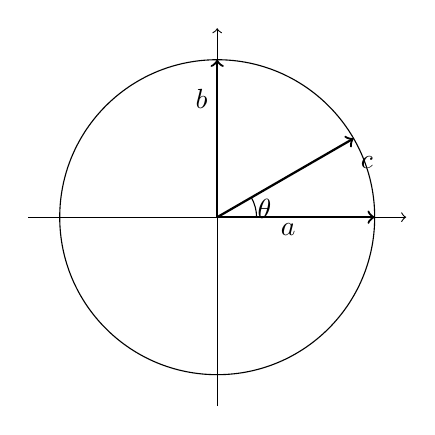
\begin{tikzpicture}[scale=2]
    % Draw coordinate axes
    \draw[->] (-1.2, 0) -- (1.2, 0); % x-axis
    \draw[->] (0, -1.2) -- (0, 1.2); % y-axis

    % Draw the unit circle
    \draw (0,0) circle(1);

    % Angle theta
    \draw[->, thick] (0,0) -- (0.866,0.5); % hypotenuse (c)
    \node at (0.95,0.35) {$c$};

    % Projection on x-axis (a)
    \draw[->, thick] (0,0) -- (1,0);
    \node at (0.45,-0.08) {$a$};

    % Projection on y-axis (b)
    \draw[->, thick] (0,0) -- (0,1);
    \node at (-0.1,0.75) {$b$};

    % Angle label θ
    \draw (0.25,0) arc[start angle=0,end angle=30,radius=0.25];
    \node at (0.3,0.05) {$\theta$};
\end{tikzpicture}
    \caption{Der initiale Zustand des Systems}
    \label{fig:initial-grover-three-qubits}
\end{figure}

Im Fall dieses Beispiels (ein System aus zwei Qubits mit dem gesuchten Index $11$) lässt sich der Zustandsvektor $c$ durch die Koordinaten $x$ und $y$ wie folgt darstellen:

$$
\frac{1}{2}(|00\rangle + |01\rangle + |10\rangle + |11\rangle) = x \cdot \frac{1}{\sqrt{3}}(|00\rangle + |01\rangle + |10\rangle) + y \cdot |11\rangle
$$

\noindent Aus dieser Gleichung ergibt sich: $x = \frac{\sqrt{3}}{2}$ und $y = \frac{1}{2}$.\\

Anhand dieser Koordinaten erkennt man, dass der Winkel $\theta$ zwischen dem Vektor $c$ und der horizontalen Achse gleich $\frac{\pi}{6}$ ist. Vorausblickend lässt sich sagen: Unser Ziel ist es, diesen Winkel auf $\frac{\pi}{2}$ (oder zumindest in dessen Nähe) zu bringen – also den Zustand nahezu vollständig in Richtung des gesuchten Basiszustands zu drehen, sodass bei der anschließenden Messung mit hoher Wahrscheinlichkeit das gewünschte Ergebnis erscheint.

Die Koordinaten des aktuellen Zustandsvektors lassen sich über den Winkel $\theta$ wie folgt beschreiben:

$$
x = \cos{\theta}
$$
$$
y = \sin{\theta}
$$

Zur Klarstellung: Der Hilfsqubit wird in der Kreisdarstellung nicht berücksichtigt, da er nicht zur Codierung des Index dient, sondern lediglich zur Markierung des gesuchten Zustands verwendet wird.

Nach Anwendung der Orakelfunktion spiegelt sich der Zustandsvektor an der horizontalen Achse. Dies liegt daran, dass seine vertikale Komponente (der Anteil des Vektors $|11\rangle$) negativ wird. Der resultierende Vektor $c_{1b}$ ist somit die Spiegelung des ursprünglichen Vektors $c$ um den Winkel $\theta$ nach unten relativ zur Horizontalen:

\begin{figure}[H]
    \centering
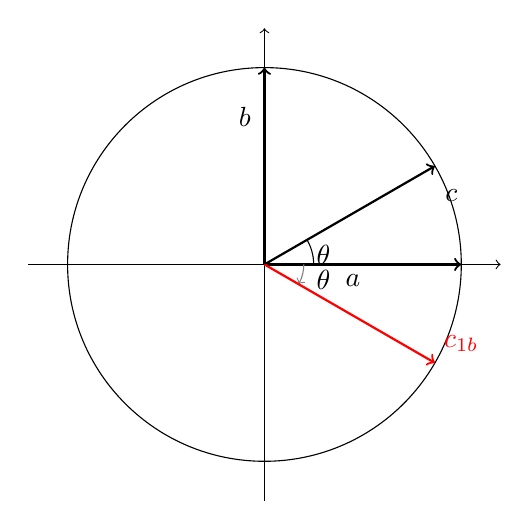
\begin{tikzpicture}[scale=2.5]

    % Draw coordinate axes
    \draw[->] (-1.2, 0) -- (1.2, 0); % x-axis
    \draw[->] (0, -1.2) -- (0, 1.2); % y-axis

    % Draw the unit circle
    \draw (0,0) circle(1);

    % Main vector c (black)
    \draw[->, thick] (0,0) -- (0.866,0.5);
    \node at (0.95,0.35) {$c$};

    % Projection on x-axis (a)
    \draw[->, thick] (0,0) -- (1,0);
    \node at (0.45,-0.08) {$a$};

    % Projection on y-axis (b)
    \draw[->, thick] (0,0) -- (0,1);
    \node at (-0.1,0.75) {$b$};

    % First angle theta
    \draw (0.25,0) arc[start angle=0,end angle=30,radius=0.25];
    \node at (0.3,0.05) {$\theta$};

    % Second angle theta (for red vector)
    \draw[gray, ->] (0.2,0) arc[start angle=0,end angle=-30,radius=0.2];
    \node at (0.3,-0.08) {$\theta$};

    % Red vector c_{1b}
    \draw[->, thick, red] (0,0) -- (0.866,-0.5);
    \node[red] at (1.0,-0.4) {$c_{1b}$};

\end{tikzpicture}
    \caption{Der Zustand des Systems nach der ersten Teil der erste Iteration}
    \label{fig:after-first-part-grover-three-qubits}
\end{figure}

Diese Spiegelung erfolgt in diesem Beispiel durch die Anwendung des $CCNOT$-Gatters. Allgemein jedoch lässt sich dieser Schritt der Orakelfunktion durch folgende Operation beschreiben:

$$
U_{1b} = I - 2|b\rangle \langle b|
$$

Hier steht $U_{1b}$ für die Orakelfunktion. Diese Operation kehrt ausschließlich das Vorzeichen der vertikalen Komponente des Zustandsvektors um, was genau zur beschriebenen Spiegelung führt.

Überprüfen wir nun die Wirkung dieser Formel anhand des Beispiels:

\begin{align*}
U_{1b} |c\rangle &= (I - 2|11\rangle \langle 11|) \cdot \frac{1}{2}(|00\rangle + |01\rangle + |10\rangle + |11\rangle) \\
&= \frac{1}{2} \left( |00\rangle + |01\rangle + |10\rangle + |11\rangle - 2|11\rangle \right) \\
&= \frac{1}{2} (|00\rangle + |01\rangle + |10\rangle - |11\rangle)
\end{align*}

Damit ist der erste Teil der Iteration abgeschlossen.

Nun wenden wir uns dem zweiten Teil der ersten Iteration zu. In diesem Schritt erfolgt eine weitere Spiegelung – jedoch nicht mehr an der horizontalen Achse, sondern am ursprünglichen Zustandsvektor $c$. Es lässt sich leicht erkennen, dass der neue Zustandsvektor danach dem Ausdruck

$$
\cos(3\theta)|a\rangle + \sin(3\theta)|b\rangle
$$

\noindent entspricht. Das bedeutet, der Winkel zwischen dem Vektor und der horizontalen Achse ist nun $3\theta$. Der Zustand wurde also weiter in Richtung des gesuchten Basiszustands $|b\rangle$ gedreht.

\begin{figure}[H]
    \centering
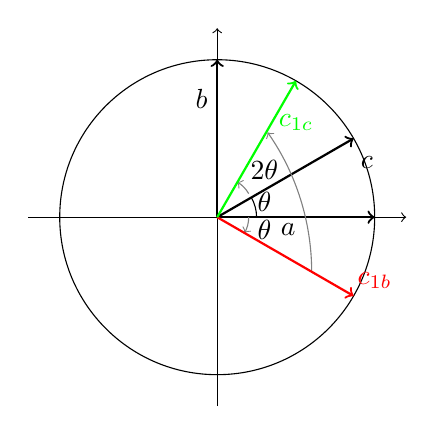
\begin{tikzpicture}[scale=2]

    % Draw coordinate axes
    \draw[->] (-1.2, 0) -- (1.2, 0); % x-axis
    \draw[->] (0, -1.2) -- (0, 1.2); % y-axis

    % Draw the unit circle
    \draw (0,0) circle(1);

    % Main vector c (black)
    \draw[->, thick] (0,0) -- (0.866,0.5);
    \node at (0.95,0.35) {$c$};

    % Projection on x-axis (a)
    \draw[->, thick] (0,0) -- (1,0);
    \node at (0.45,-0.08) {$a$};

    % Projection on y-axis (b)
    \draw[->, thick] (0,0) -- (0,1);
    \node at (-0.1,0.75) {$b$};

    % First angle theta
    \draw (0.25,0) arc[start angle=0,end angle=30,radius=0.25];
    \node at (0.3,0.1) {$\theta$};

    % Second angle theta (for red vector)
    \draw[gray, ->] (0.2,0) arc[start angle=0,end angle=-30,radius=0.2];
    \node at (0.3,-0.08) {$\theta$};

    % Third angle theta (for red vector)
    \draw[gray, ->] (0.2,0.15) arc[start angle=30,end angle=60,radius=0.2];
    \node at (0.3,0.3) {$2\theta$};

    \draw[gray, ->] (0.6,-0.35) arc[start angle=0,end angle=35,radius=1.55];

    % Red vector c_{1b}
    \draw[->, thick, red] (0,0) -- (0.866,-0.5);
    \node[red] at (1.0,-0.4) {$c_{1b}$};

    % Green vector c_{1c}
    \draw[->, thick, green] (0,0) -- (0.5,0.866);
    \node[green] at (0.5,0.6) {$c_{1c}$};

\end{tikzpicture}
    \caption{Der Zustand des Systems nach der zweiten Teil der erste Iteration}
    \label{fig:after-second-part-grover-three-qubits}
\end{figure}
Die Operation zur Erzeugung des reflektierten Vektors $c_{1c}$ sieht wie folgt aus:

$$
U_{1c} = 2|c\rangle \langle c| - I
$$

Berechnen wir den resultierenden Vektor $c_{1c}$ für unser Beispiel:

\begin{align*}
U_{1c} |c_{1b}\rangle &= \left(2|c\rangle \langle c| - I\right) \cdot \frac{1}{2} (|00\rangle + |01\rangle + |10\rangle - |11\rangle) \\
&= |11\rangle
\end{align*}

Es fand eine Spiegelung des Zustandsvektors $|c_{1b}\rangle$ an $|c\rangle$ statt. Wenn man den Vektor $|c_{1b}\rangle$ als Linearkombination $k_1 |c\rangle + k_2 |c_{\perp}\rangle$ schreiben kann, wobei $|c_{\perp}\rangle$ senkrecht auf $|c\rangle$ steht und $k_1$, $k_2$ reelle Koeffizienten sind, dann ergibt sich der gespiegelte Vektor zu:

$$
k_1 |c\rangle - k_2 |c_{\perp}\rangle
$$

Genau dies geschieht hier: Die Komponente entlang $|c\rangle$ bleibt erhalten, während die senkrechte Komponente ihr Vorzeichen ändert. In unserer Quantenschaltung wird dieser zweite Teil der Iteration folgendermaßen implementiert:

\begin{figure}[h!]
    \centering
    \includegraphics[width=0.4\textwidth]{images/basic-algorithms/grover-2-iteration.png}
    \caption{Zweite Iteration - $U_{1c}$}
    \label{fig:grover-second-iteration}
\end{figure}

Zunächst wird der Hadamard-Operator auf den ersten und zweiten Qubit angewendet. Dies vereinfacht unsere Aufgabe erheblich, da die Reflexion des Zustandsvektors nun nicht mehr relativ zum Superpositionszustand $\frac{1}{2}(|00\rangle + |01\rangle + |10\rangle + |11\rangle)$ erfolgen muss, sondern relativ zum Zustand $|00\rangle$.

Um die Spiegelung durchzuführen, müssten wir eigentlich allen Zuständen außer dem Nullzustand ein negatives Vorzeichen zuweisen. Stattdessen nutzen wir jedoch einen Trick: Wir versehen lediglich den Zustand $|00\rangle$ mit einem Minuszeichen und lassen alle übrigen Superpositionszustände unverändert. Dies erreichen wir durch eine gezielte Abfolge von Gattern: zuerst $X$-Gatter, dann ein $CCNOT$-Gatter, und danach wird die Transformation durch Umkehr der Schritte rückgängig gemacht – also erneut $X$-Gatter und anschließend Hadamard-Gatter.

Aufgrund dieses Tricks (Negation nur des Nullzustands) ergibt sich in unserem Beispiel mit zwei Qubits nicht $|11\rangle$, sondern $-|11\rangle$ als Ergebnis – abgesehen von einer globalen Phase. Dies ist jedoch unproblematisch, da sich die globale Phase beim Messen nicht auswirkt und wir den gesuchten Index trotzdem korrekt erhalten.

Aus der Darstellung auf dem Einheitskreis, die den Zustand des Systems nach der zweiten Hälfte der ersten Iteration veranschaulicht, wird deutlich, dass der Zustandsvektor mit jeder weiteren Iteration der Vertikalen näherkommt. In unserem konkreten Fall beträgt der Winkel zwischen Zustandsvektor und Horizontaler nach Abschluss der ersten Iteration bereits $3\theta$, was genau dem gewünschten Winkel $\frac{\pi}{2}$ entspricht.

Im allgemeinen Fall ergibt sich der Winkel nach $t$ Iterationen zu:

$$
(2t + 1)\theta \approx \frac{\pi}{2}
$$

Daraus lässt sich die erforderliche Anzahl an Iterationen für den Grover-Algorithmus bestimmen. Wenn $t$ groß ist und $K = 1$ (für $K > 1$ ist der Schluss analog), wird der Winkel $\theta$ sehr klein. Daher kann man $\theta$ durch $\sin{\theta}$ ersetzen, und es gilt näherungsweise:

$$
\theta \approx \sin{\theta} = \frac{1}{\sqrt{N}}
$$

Daraus folgt:

$$
(2t + 1) \cdot \frac{1}{\sqrt{N}} \approx \frac{\pi}{2}
$$

Wenn man die Eins im Term $(2t + 1)$ vernachlässigt (für große $t$ zulässig), erhält man:

$$
t \approx \frac{\pi \sqrt{N}}{4}
$$

Wie wir bereits gesehen haben, besteht jede Iteration aus zwei Schritten. Der erste Schritt ist die Reflexion nach unten an der Horizontalen. Der zweite Schritt ist die Reflexion nach oben an der ursprünglichen Richtung, also am Vektor $c$. Dabei wird der Zustandsvektor stets auf einen größeren Winkel nach oben reflektiert als der Winkel der vorherigen Spiegelung nach unten. Genau dadurch nähert sich der Vektor bei jeder Iteration schrittweise der Vertikalen.\\

Wir haben ein Beispiel für die Anwendung des Grover-Algorithmus betrachtet. Im nächsten Kapitel werden wir uns mit der Zeitkomplexität beschäftigen und erläutern, warum dieser Algorithmus trotz der Anzahl an Iterationen dennoch schneller ist als klassische Suchalgorithmen.


\subsection{Komplexitätsanalyse}
Der Grover‐Algorithmus durchsucht eine unstrukturierte Datenbank der Größe \(N\) mithilfe eines Quantenorakels in \(\Theta(N)\) Orakelaufrufen. Anders ausgedrückt: Während die klassische Vollsuche im Mittel \(\Theta(N)\) Prüfungen erfordert, reduziert Grover die Zahl der notwendigen Prüfungen auf etwa $\frac{\pi}{4}\,\sqrt{N}\ $ das heißt auf die Quadratwurzel der Datenbankgröße.

Aus Sicht der Komplexitätstheorie bezeichnet man die Eingangsgröße mit \(n\), so dass $N = 2^n$.
Die Laufzeit des Grover‐Algorithmus lässt sich daher durch  
$O\bigl(2^{n/2}\bigr)$ beschreiben. Obwohl dies gegenüber dem klassischen \(O(2^n)\) einen erheblichen quadratischen Gewinn darstellt, wächst der Algorithmus bei zunehmender Zahl der Suchbits weiterhin exponentiell.

Die untere Schranke aus der Arbeit von Bennett–Bernstein–Brassard–Vazirani (BBBV96 referenz) zeigt, dass kein Quantenalgorithmus im Black‐Box‐Modell mit weniger als  
\[
\Omega(\sqrt{N})
\]  
Orakelaufrufen auskommen kann. Damit ist der Grover‐Algorithmus in diesem Modell asymptotisch optimal: Ohne zusätzliche Struktur in der Datenbank lässt sich kein suprakquadratischer (etwa exponentieller) Vorteil erzielen.  


\section{Klassifikation von Algorithmen nach Zeitkomplexität}

Im Rahmen der theoretischen Informatik werden Entscheidungsprobleme nach der zur Lösung benötigten Zeit in verschiedene Klassen eingeordnet. Dabei interessiert insbesondere, welche Probleme auf einem klassischen bzw. quantenmechanischen Modell in polynomieller Zeit lösbar sind, und wie sich diese Klassen zueinander verhalten.\\

Zunächst versteht man unter der Klasse \(\mathbf{P}\) jene Probleme, für die es deterministische Algorithmen gibt, die auf einem klassischen Computer in polynomieller Zeit laufen. Formal heißt das: Ein Problem liegt in \(\mathbf{P}\), wenn es einen Algorithmus gibt, dessen Laufzeit durch einen Polynomausdruck \(O(n^k)\) für eine feste Konstante \(k\) beschränkt ist, wobei \(n\) die Eingabegröße bezeichnet. Probleme aus \(\mathbf{P}\) gelten als praktisch effizient lösbar, sofern der Exponent \(k\) nicht zu groß wird.\\

Die Klasse \(\mathbf{NP}\) (nondeterministic polynomial time) umfasst diejenigen Entscheidungsprobleme, bei denen eine etwaige Lösung auf einem klassischen Computer in polynomieller Zeit verifizierbar ist, auch wenn ein deterministischer polynomieller Lösungsalgorithmus bislang unbekannt ist. Ein typisches Beispiel ist das Teilmengen-Summen-Problem: Legt man dem Algorithmus als „Zertifikat“ eine vermutete Teilmenge vor, so kann man in \(O(n)\) bzw. \(O(n\log n)\) Zeit nachprüfen, ob die Summe den Zielwert ergibt.\\

Innerhalb von \(\mathbf{NP}\) existieren die \(\mathbf{NP}\)-\emph{vollständigen} Probleme (\(\mathbf{NP}\)\emph{-complete}), die zu den schwierigsten \(\mathbf{NP}\)-Problemen zählen. Ein Problem \(L\) ist genau dann \(\mathbf{NP}\)-vollständig, wenn \(L\in\mathbf{NP}\) und jedes andere Problem aus \(\mathbf{NP}\) in polynomieller Zeit auf \(L\) reduziert werden kann. Die berühmte \textsc{Clique}-Frage oder das \textsc{3-SAT}-Problem sind klassische Vertreter dieser Klasse. Gelingt es, eines dieser Probleme in polynomieller Zeit zu lösen, so hätte man damit einen polynomiellen Algorithmus für alle \(\mathbf{NP}\)-Probleme.\\

Die Klasse der \(\mathbf{NP}\)-\emph{harten} Probleme (\(\mathbf{NP}\)\emph{-hard}) enthält solche Probleme, auf die sich beliebige \(\mathbf{NP}\)-Probleme in polynomieller Zeit reduzieren lassen. Im Gegensatz zu \(\mathbf{NP}\)-vollständigen Problemen müssen \(\mathbf{NP}\)-harte Probleme selbst nicht in \(\mathbf{NP}\) liegen und können etwa gar nicht entscheidbar sein oder nur in exponentieller Zeit verifizierbar sein.\\

Wenn man zusätzlich zur deterministischen Rechenmaschine Zufallsbits zulässt und die Wahrscheinlichkeit, die richtige Entscheidung zu treffen, für positive und negative Instanzen jeweils oberhalb eines festen Schwellwerts (typischerweise \(>1/2\)) liegt, definiert man die Klasse \(\mathbf{BPP}\) (bounded‑error probabilistic polynomial time). Probleme in \(\mathbf{BPP}\) lassen sich mit Monte‑Carlo‑Algorithmen in polynomieller Zeit mit beliebig kleiner Fehlerrate lösen.\\

Der quantenmechanische Gegenpart zu \(\mathbf{BPP}\) ist die Klasse \(\mathbf{BQP}\) (bounded‑error quantum polynomial time). Hierbei kann ein Quantenalgorithmus für ein Problem in polynomieller Zeit auf einem Quantencomputer mit hoher Wahrscheinlichkeit das korrekte Ergebnis liefern. Ein bekanntes Beispiel ist die Ganzzahlfaktorzerlegung großer Zahlen mittels Shor’s Algorithmus, der das hierfür klassische \(\mathbf{NP}\)-Problem in polynomieller Zeit auf einem Quantencomputer löst.

\begin{figure}[h]
  \centering
  \includegraphics[width=0.7\textwidth]{images/basic-algorithms/problem-classes.png}
  \caption{Übersicht der wichtigsten Zeitkomplexitätsklassen: \(\mathbf{P}\subseteq \mathbf{BQP}\subseteq \mathbf{NP}\subseteq \mathbf{NP}\text{-hard}\) und die Lage von \(\mathbf{NP}\)-complete Problemen innerhalb von \(\mathbf{NP}\).}
  \label{fig:problem_classes}
\end{figure}

Abschließend lässt sich festhalten, dass die Frage, ob \(\mathbf{P}=\mathbf{NP}\) gilt, zu den bedeutendsten offenen Problemen der Informatik zählt. Auch der Vergleich zwischen klassischen und quantenmechanischen Modellen, speziell die Vermutung \(\mathbf{P}\subsetneq \mathbf{BQP}\subseteq \mathbf{NP}\), prägt die Forschung im Bereich effizienter Algorithmen maßgeblich.

\section{Quantum Safe Algorithmen}

\subsection*{Einleitung}

Mit der rasanten Entwicklung von Quantencomputern stehen klassische Verschlüsselungsverfahren vor einer existenziellen Bedrohung. Während heutige Systeme auf der Annahme beruhen, dass bestimmte mathematische Probleme schwer zu lösen sind, können Quantenalgorithmen wie \textit{Shor’s Algorithmus} oder \textit{Grover’s Algorithmus} diese Probleme effizient berechnen – und damit die Sicherheit brechen, auf die heutige digitale Kommunikation angewiesen ist.

Diese Bedrohung macht sogenannte \textbf{Quantum Safe Algorithmen} notwendig – kryptographische Verfahren, die auch gegen Angriffe durch leistungsfähige Quantencomputer resistent sind. Zwei Hauptansätze stehen im Zentrum der Forschung:

\begin{itemize}
  \item \textbf{Quantum Key Distribution (QKD)} – ein Verfahren, das physikalische Gesetze der Quantenmechanik nutzt, um absolut sichere Schlüsselverteilungen zu ermöglichen.
  \item \textbf{Post-Quantum Cryptography (PQC)} – klassische, quantenresistente Algorithmen, die auf heutigen Geräten ausgeführt werden können.
\end{itemize}

In diesem Kapitel werfen wir einen Blick auf beide Ansätze – und erläutern insbesondere die jüngsten Fortschritte durch das NIST (National Institute of Standards and Technology), das 2022 erste standardisierungsreife Algorithmen bekannt gegeben hat.

\subsection{Quantum Key Distribution}

Quantum Key Distribution (QKD) ermöglicht es, kryptografische Schlüssel über unsichere Kanäle zu übertragen – mit einem entscheidenden Vorteil: Jeder Abhörversuch verändert unweigerlich den Zustand der übertragenen Quanteninformation und kann somit erkannt werden.

Ein klassisches Beispiel für ein QKD-Protokoll ist das \textbf{BB84-Protokoll}, das 1984 von Bennett und Brassard entwickelt wurde und später, im Jahr 2000, von Peter W. Shor and John Preskill geprüft wurde. Es nutzt die Polarisation von Photonen, um binäre Informationen zu codieren. Der Ablauf besteht aus drei Phasen:

\begin{itemize}
  \item \textbf{Key Exchange:} Alice sendet zufällig polarisierte Photonen an Bob, der sie in zufällig gewählten Basen misst.
  \item \textbf{Key Sifting:} Über einen klassischen Kanal gleichen beide ihre verwendeten Basen ab und behalten nur die Werte, bei denen die Basen übereinstimmten.
  \item \textbf{Key Distillation:} Durch Stichproben wird geprüft, ob Abhörversuche stattfanden. Die finale Schlüssellänge ergibt sich nach dieser Bereinigung.
\end{itemize}

\noindent Neben BB84 existieren weitere bedeutende Protokolle:

\begin{itemize}
  \item \textbf{B92} (reduzierte Variante mit zwei Zuständen)
  \item \textbf{E91} (nutzte erstmals Quantenverschränkung)
  \item \textbf{BBM92}, \textbf{SARG04}, \textbf{DPS}, \textbf{COW}, \textbf{GG02} (verschiedene Weiterentwicklungen)
\end{itemize}

Für eine detaillierte Übersicht der Protokolle und deren Unterschiede siehe das Paper:
\textit{An Overview of Quantum-Safe Approaches: Quantum Key Distribution and Post-Quantum Cryptography} von Guobin Xu et al.

\subsection{Post-Quantum Cryptographie Algorithmen}

Da QKD mit hohen technischen und infrastrukturellen Anforderungen verbunden ist, setzt sich in der Praxis vor allem die \textbf{Post-Quantum Cryptography (PQC)} durch. Sie nutzt klassische Rechenverfahren, basiert jedoch auf mathematischen Problemen, die auch für Quantencomputer als schwierig gelten.

Das US-amerikanische \textbf{NIST} hat im Rahmen eines mehrjährigen Wettbewerbs Verfahren für zwei Hauptkategorien gesucht:

\begin{itemize}
  \item \textbf{Public-Key Encryption and Key Establishment (KEM)}
  \item \textbf{Digitale Signaturverfahren}
\end{itemize}

\noindent Nach mehreren Runden wählte NIST im Juli 2022 vier Algorithmen aus, die als erste Quantum Safe Standards empfohlen werden.

\noindent Für Verschlüsselung und Schlüsselaustausch nominierte NIST:

\begin{itemize}
  \item \textbf{CRYSTALS-Kyber} – 2017, J. Bos et al.
\end{itemize}

\vspace{0.5em} % optionaler vertikaler Abstand

\noindent Für digitale Signaturen nominierte NIST:

\begin{itemize}
  \item \textbf{CRYSTALS-Dilithium} – 2018, L. Ducas et al.

  \item \textbf{Falcon} – 2018, P.-A. Fouque et al.

  \item \textbf{SPHINCS+} – 2019, D. J. Bernstein et al.
\end{itemize}

\subsubsection*{CRYSTALS-Kyber}

\textbf{CRYSTALS-Kyber} ist ein \textit{lattice-basiertes Key Encapsulation Mechanism (KEM)}. Es basiert auf dem sogenannten \textit{Module Learning with Errors (MLWE)}-Problem, das auch von Quantencomputern bislang nicht effizient gelöst werden kann.

Der Algorithmus nutzt Polynomarithmetik und besteht aus drei Hauptschritten:

\begin{enumerate}
  \item \textbf{Schlüsselerzeugung:} Öffentlicher und privater Schlüssel werden erzeugt.
  \item \textbf{Encapsulation:} Ein gemeinsamer Schlüssel wird erzeugt und verschlüsselt übertragen.
  \item \textbf{Decapsulation:} Der Empfänger entschlüsselt den Schlüssel mit seinem privaten Schlüssel.
\end{enumerate}

\noindent Kyber bietet drei Sicherheitsniveaus, die sich durch unterschiedliche Parametergrößen unterscheiden und an klassische AES-Sicherheitsstufen angelehnt sind:

\begin{itemize}
  \item \textbf{Kyber-512} – Sicherheitsniveau 1 (vergleichbar mit AES-128)
  \item \textbf{Kyber-768} – Sicherheitsniveau 3 (vergleichbar mit AES-192)
  \item \textbf{Kyber-1024} – Sicherheitsniveau 5 (vergleichbar mit AES-256)
\end{itemize}

\subsubsection*{CRYSTALS-Dilithium}

\textbf{CRYSTALS-Dilithium} ist ein digitaler Signaturalgorithmus, ebenfalls basierend auf \textit{MLWE} und \textit{MSIS} (Module Short Integer Solution). Die Signaturerzeugung verwendet die \textit{Fiat-Shamir-Transformation}, die aus einem interaktiven Zero-Knowledge-Protokoll eine nicht-interaktive Signatur macht.

Dilithium bietet drei Sicherheitsniveaus:

\begin{itemize}
  \item \textbf{Dilithium2}
  \item \textbf{Dilithium3}
  \item \textbf{Dilithium5}
\end{itemize}

Die Vorteile liegen in der schnellen Verifikation, der Robustheit gegen Seitenkanalangriffe und der guten Performance. Diese Eigenschaften machen Dilithium zu einem führenden Kandidaten im Bereich der quantensicheren digitalen Signaturen.
\printbibliography
%\motto{Use the template \emph{chapter.tex} to style the various elements of your chapter content.}
\chapter{Quantensoftware und Programmierung}
\label{programming} % Always give a unique label
% use \chaptermark{}
% to alter or adjust the chapter heading in the running head

\chapterauthor{Konrad Maywald, Daniel Purtov, Dennis Schweigert, Tom Williard}

\abstract{some abstract}

\section{Programmiermodelle in der Quanteninformatik}
\label{programming-models}
\subsection{Gate-basiertes Paradigma (Quantum Circuit Model)}
Das Gate-basierte Paradigma oder auch Quantenschaltkreis Modell (engl. Quantum Circuit Model) genannt, ist das Standardmodell für die Programmierung von Quantenprogrammen. Daher wird es auch häufig als das am weitesten verbreitete Paradigma in der Quanteninformatik zur Beschreibung und Realisierung von Quantenalgorithmen bezeichnet. In diesem Modell werden die Quantenprogramme als Schaltkreise (engl. quantum circuits) dargestellt. Diese bestehen aus einer Sequenz von unitären Quanten-Gattern, welche auf Qubits angewendet werden. 

Strukturell orientiert sich das Quantenschaltkreismodell an klassischen digitalen Schaltungen. Klassische Schaltkreise bestehen aus Leitungen, Gattern und Bits mit den Zuständen 0 und 1. Analog dazu bestehen Quantenschaltkreise aus Qubit-Leitungen, Gattern und Quantenbits (Qubits). Jede Leitung repräsentiert dabei ein Qubit und jedes Gatter eine unitäre Transformation auf eines oder mehrere Qubits. Die Struktur des Quantenschaltkreises wird meist visuell dargestellt, um die Reihenfolge der angewendeten Operationen und die daran beteiligten Qubits zu verdeutlichen.

\begin{figure}[ht!]
    \centering
    \includegraphics[width=0.5\linewidth]{images/qubit_gates.png}
    \caption{Qubit Gates \autocite[177]{nielsen_quantum_2010}}
    \label{fig:enter-label}
\end{figure}

\autoref{fig:enter-label} zeigt typische elementare Gates, welche für die Konstruktion von Quantenschaltkreisen verwendet werden. Das Hadamard-Gate (H) bringt Qubits aus ihren Basiszuständen in eine Superposition. Das CNOT-Gate (Controlled-Not) ist ein Gate mit zwei Qubits, das diese miteinander verschränkt und so als zentraler Bestandteil der Quantenverschränkung fungiert. Darüber hinaus gibt es weitere Gates wie die Pauli-X-, -Y- und -Z-Gates, Phasengatter und das T-Gate. Werden mehrere dieser Gatter nacheinander auf ein Qubit-Register angewendet, bildet sich daraus ein Quanten-Schaltkreis, welcher als Quantenalgorithmus verstanden werden kann. \autocite[174-188]{nielsen_quantum_2010}

\textbf{Brauchen wir das so? Das doppelt sich glaube ich sehr mit der Algorithmen-Gruppe}

\subsection*{Bekannte Quantenalgorithmen basierend auf dem Quantenschaltkreismodell}

Das Quantenschaltkreismodell dient als Grundlage für mehrere bekannte Quantenalgorithmen dazu zählen folgende: (siehe auch (\autoref{basic_algorithms}))
\subsubsection*{1) Shor's Algorithmus}
Der Shor Algorithmus führt eine effiziente Primfaktorzerlegung großer Zahlen durch, was klassische Verschlüsselungsverfahren wie RSA bedroht. Der Algorithmus verwendet die Quantum Fourier Transformation (QFT) und periodenfindende Subroutinen innerhalb des Circuit-Models. (siehe auch (\autoref{first:shor-algorithm}) \autocite[226-232]{nielsen_quantum_2010} \autocite{haywardQuantumComputingShors2005}

\subsubsection*{2) Grover´s Algorithmus}
Der Grover Algorithmus dient zur Suche eines Eintrags in einer unstrukturierten Datenbank mit einer quadratischen Beschleunigung gegenüber klassischen Verfahren.
Der Algorithmus basiert auf Rotation in einem zweidimensionalen Unterraum, dargestellt als wiederholte Anwendung von sogenannten Grover-Iterationen, realisiert durch Gates im Circuit-Modell. (ausführliche Erklärung: (\autoref{sec:grover-algorithm}))  \autocite[248-254]{nielsen_quantum_2010}

\subsubsection*{3) Regev}
Regevs Arbeiten zum LWE-Problem beinhalten eine theoretische Quantenreduktion, die sich vollständig im gate-basierten Modell realisieren lässt. Die dafür erforderlichen Operationen – wie das Erzeugen von Superpositionen, die Anwendung der Quanten-Fouriertransformation sowie die Verarbeitung von Messresultaten – sind mit klassischen Quanten-Gattern (z.B. Hadamard-, CNOT- und Phasengattern) darstellbar. Auch wenn Regevs Reduktion primär theoretischer Natur ist und keine praktischen Implementierungen wie Shor oder Grover hat, zeigen die verwendeten Techniken eine klare Kompatibilität mit dem Quantum Circuit Model. \autocite{regev_lattices_2024}

\textbf{TODO ENDE}
\\
\\
Das Gate-basierte Paradigma ist nicht nur ein theoretisches Modell, sondern spielt auch in der Praxis eine zentrale Rolle. So setzt zum Beispiel das Open-Source-Framework Qiskit von IBM auf dieses Modell. Quantenprogramme werden dort als sogenannte \enquote{Quantum Circuits} aufgebaut. Diese bestehen aus einer festen Anzahl von Qubits und einer Folge von Operationen, also Gattern, Messungen und Resets -- genau wie es im Schaltkreis-Modell vorgesehen ist. Das Gate-basierte Modell ist nicht nur für die Entwicklung von Algorithmen wichtig, sondern auch für den praktischen Einsatz auf echten Quantencomputern, wie denen von IBM oder Google.

\subsection{Messungsbasiertes Paradigma}
Das messungsbasierte Paradigma, auch bekannt als \textit{Measurement-Based Quantum Computing (MBQC)} oder \textit{One-Way Quantum Computation}, stellt eine alternative Architektur zur Implementierung von Quantenalgorithmen dar. Im Gegensatz zum weit verbreiteten Schaltkreis-Modell, bei dem Quanteninformationen durch sequenzielle Anwendung unitärer Gatter verarbeitet werden, basiert MBQC auf einer anderen Grundidee: Der eigentliche Rechenprozess erfolgt nicht durch Gatter, sondern ausschließlich durch gezielte Einzelqubit-Messungen an einem vorbereiteten, verschränkten Vielteilchenzustand – dem sogenannten Cluster-State.

Diese Struktur eröffnet neue Möglichkeiten für die Organisation und Steuerung von Quanteninformation. Die gesamte logische Verarbeitung geschieht dabei einseitig (\enquote{one-way}), da jede Messung irreversibel ist und den gemessenen Qubit-Zustand zerstört. Die Fähigkeit zur universellen Quantenberechnung wird vollständig durch die Verschränkungseigenschaften des vorbereiteten Zustands sowie die geschickte Wahl und Abfolge der Messungen realisiert. \autocite[2-4]{briegelMeasurementbasedQuantumComputation2009}

\subsection*{Struktur und Erzeugung von Cluster-States}
Die zentrale Ressource des MBQC ist der Cluster-State, ein hochgradig verschränkter Quantenzustand mehrerer Qubits. Formal gehört der Cluster-State zur Klasse der Graphenzustände. Diese Zustände lassen sich durch mathematische Graphen beschreiben, in denen Knoten einzelnen Qubits entsprechen und Kanten die Verschränkungen zwischen ihnen darstellen. Die Erzeugung eines solchen Zustands erfolgt in zwei Schritten:

\begin{enumerate}
    \item Überführung aller Qubits in den Zustand $|+\rangle = \frac{1}{\sqrt{2}}(|0\rangle + |1\rangle)$
    \item Anwendung eines kontrollierten Phasengatters $U_{PG}=diag(1,1,1,-1)$ auf jedes benachbarte Qubit-Paar (gemäß der Graphenstruktur)
\end{enumerate}

Der so erzeugte Zustand $|G\rangle$ (G ist der zugrundeliegende Graph) besitzt die gewünschten Verschränkungseigenschaften, um ihn als Rechenressource im MBQC zu verwenden. Besonders der zweidimensionale Cluster-State hat sich hierbei als universell erwiesen und kann für die Implementierung beliebiger Quantenalgorithmen verwendet werden. \autocite[2-3]{briegelMeasurementbasedQuantumComputation2009}

\subsection*{Rechenmodell und Algorithmus Implementierung}

Eine MBQC-Berechnung lässt sich in einem schematischen Ablauf darstellen, der vier grundlegende Schritte umfasst:
\begin{enumerate}
    \item \textbf{Initialisierung:} Vorbereitung eines ausreichend großen 2D-Cluster-States, der unabhängig vom konkreten Algorithmus erzeugt wird.
    \item \textbf{Kodierung des Algorithmus durch Messmuster:} Die Berechnung wird durch eine Sequenz von Einzelqubit-Messungen in ausgewählten Basen realisiert. Dabei bestimmt das Muster der Messungen (also deren Reihenfolge und jeweilige Basis) die Art der durchgeführten logischen Operationen.
    \item \textbf{Adaptive Steuerung:} Die Wahl der Messbasis für spätere Schritte kann von den Ergebnissen vorheriger Messungen abhängen. Diese Feedforward-Kontrolle wird durch eine klassische Recheneinheit übernommen.
    \item \textbf{Ausgabezustand:} Das Endresultat der Quantenberechnung ist entweder in den verbleibenden nicht gemessenen Qubits codiert oder ergibt sich aus den Messergebnissen selbst. Die resultierenden Zustände unterscheiden sich maximal durch lokale Pauli-Operationen.
\end{enumerate}

Ein bemerkenswertes Merkmal dieses Modells ist, dass trotz der inhärenten Zufälligkeit der einzelnen Messergebnisse aufgrund des quantenmechanischen Messprozesses der gesamte Rechenvorgang deterministisch kontrolliert und wiederholbar bleibt – vorausgesetzt, das Feedforward wird korrekt berücksichtigt. \autocite[3-4]{briegelMeasurementbasedQuantumComputation2009}

\subsection*{Exemplarische Anwendungen}

Das Potenzial des MBQC lässt sich gut an ausgewählten Beispielen verdeutlichen. Eines der grundlegendsten Konzepte ist das Teleportationsprotokoll, das im Kontext des MBQC zeigt, wie Quanteninformation durch Messungen effektiv von einem Teil des Clusters zum anderen übertragen werden kann. Dieses Prinzip bildet die Basis für viele weiterführende Techniken, darunter auch die Realisierung effektiver logischer Gatter allein durch Messungen.

Darüber hinaus lassen sich bekannte Algorithmen wie der Shor-Algorithmus zur Faktorisierung großer Zahlen oder der Grover-Algorithmus zur Datenbanksuche in messungsbasierten Varianten formulieren. Diese benötigen lediglich eine geeignete Struktur des zugrunde liegenden Cluster-States sowie eine korrekt gewählte Messstrategie, um dieselbe Funktionalität wie im Schaltkreis-Modell abzubilden. Damit zeigt sich die formale Äquivalenz der beiden Paradigmen bei grundlegend unterschiedlicher Umsetzung. \autocite[2]{briegelMeasurementbasedQuantumComputation2009}

\subsection{Adiabatisches Paradigma (Quantum Annealing)}

Ein weiteres Modell zur Realisierung von Quantenalgorithmen ist das adiabatische Paradigma, welches auch als \enquote{Quantum Annealing} bezeichnet wird. Das adiabatische Modell basiert auf der Idee, ein Quantensystem durch eine langsame, kontinuierliche Änderung eines Hamiltonians gezielt in seinen Grundzustand zu führen. Die gesuchte Lösung des Modells ist in diesem Grundzustand markiert, was das Quantum Annealing vom Gate- oder messungsbasierten Modell unterscheidet.

Beim Quantum Annealing wird das Quantensystem zunächst in einem leicht vorbereiteten Anfangszustand gehalten. Dieser entspricht dem Grundzustand eines sogenannten treibenden Hamiltonians $H_D$. Dieser Hamiltonian kann z.B. ein transversales Feld enthalten, das alle Qubits gleichmäßig beeinflusst. Im Laufe des Algorithmus wird danach schrittweise der Problem-Hamiltonian $H_P$ zugeschaltet. Dieser enthält die Struktur des zu lösenden Problems. Die Gesamtentwicklung erfolgt über einen zeitabhängigen Hamiltonian (\autoref{eq:time-dependent-hamiltonian}). 

\begin{equation}
    H(t) = A(t) \cdot H_D + B(t) \cdot H_P
\label{eq:time-dependent-hamiltonian}
\end{equation}

Die beiden Funktionen A(t) und B(t) steuern, wie stark der jeweilige Hamiltonian zu einem bestimmten Zeitpunkt t wirkt. Am Anfang dominiert hierbei $H_D$ und am Ende $H_P$. Das System bleibt nach dem adiabatischen Theorem während des gesamten Prozesses im jeweiligen Grundzustand, wenn die Änderungen langsam genug erfolgen. Am Ende wird die gesuchte Lösung, der Grundzustand von $H_P$, erreicht.
 
Die Änderungsgeschwindigkeit, mit der die Hamiltonians modifiziert werden dürfen, hängt stark vom sogenannten Energieabstand (Gap) zwischen dem Grundzustand und dem ersten angeregten Zustand ab. Je kleiner dieser Abstand ist, desto langsamer muss die Änderung erfolgen, um unerwünschte Übergänge in angeregte Zustände zu vermeiden.

Das Quantum Annealing eignet sich besonders gut für kombinatorische Optimierungsprobleme, da diese oftmals auf sogenannte Ising-Modelle abgebildet werden können. Ein Problem-Hamiltonian kann beispielsweise die in \autoref{eq:problem-hamiltonian} dargestellte Form annehmen. Die Kopplungsterme $J_{ij}$ und die lokalen Felder $h_i$ kodieren hierbei die jeweilige Problemstruktur. \autoref{tab:qa-problems} stellt eine Auswahl von Problemklassen dar, die mittels Quantum Annealing gelöst werden können.

\begin{equation}
H_P = \sum_{i,j} J_{ij}\sigma_i^z\sigma_j^z + \sum_i h_i\sigma_i^z
\label{eq:problem-hamiltonian}
\end{equation}

\begin{table}[ht!]
\centering
\begin{tabularx}{\textwidth}{|l|X|}
\hline
\textbf{Problemklasse} & \textbf{Beschreibung} \\
\hline
Max-Cut & Zerlegung eines Graphen in zwei Teilmengen mit maximaler Kantensumme zwischen ihnen. \\
\hline
k-Clique & Finden eines vollständigen Teilgraphen mit genau \(k\) Knoten. \\
\hline
Graph Coloring & Einfärben von Knoten, sodass benachbarte Knoten verschiedene Farben erhalten. \\
\hline
Ising-Minimierung & Direktes Minimieren des Ising-Hamiltonians, auf den sich viele kombinatorische Probleme abbilden lassen. \\
\hline
\end{tabularx}
\caption{Typische kombinatorische Probleme für Quantum Annealing}
\label{tab:qa-problems}
\end{table}

Quantum Annealing (QA) verwendet im Gegensatz zum klassischen Simulated Annealing (SA) Quantenfluktuationen (z. B. Quanten-Tunnel), um Energiebarrieren zu überwinden. Dies ist vor allem dann ein Vorteil, wenn die Energiebarrieren hoch, aber schmal sind. In diesen Fällen kann das Quantum Annealing schneller eine optimale Lösung finden als sein klassisches Gegenstück Simulated Annealing. Das adiabatische Paradigma wurde in der Praxis unter anderem durch die Firma D-Wave Systems in Hardware umgesetzt. \autocite[2-4]{rajak_quantum_nodate} \autocite[4-5, 42-43]{albash_adiabatic_2018}

\subsection{Hybrid-Paradigma}

Ein weiterer Ansatz zur Realisierung von Quantenalgorithmen ist das Hybrid-Paradigma. Es ist besonders interessant, weil es sowohl klassische als auch quantenmechanische Bestandteile kombiniert. Konkret laufen die aufwendigen und hardwareintensiven Berechnungen wie die Manipulation und Messung von Quantenzuständen auf dem Quantencomputer, während Aufgaben wie das Anpassen von Parametern oder das Auswerten von Messergebnissen klassisch bearbeitet werden. Aufgrund dieser Aufgabenteilung lassen sich viele Probleme bereits heute auf existierender Hardware lösen. Das liegt vor allem daran, dass das Hybrid-Paradigma mit kurzen Quantenschaltungen auskommt und keine langen kohärenten Entwicklungen benötigt. \autocite[1-2]{cerezo_variational_nodate}

Den Ausgangspunkt beim Hybrid-Paradigma bildet ein Anfangszustand, der mithilfe einer parametrierten Quantenschaltung erzeugt wird. Anschließend wird ein Zielwert gemessen und an den klassischen Computer zurückgegeben. Auf diesem wird dann ein Optimierungsalgorithmus ausgeführt, der neue Parameter vorschlägt, mit denen die Quantenschaltung beim nächsten Durchlauf verändert wird. Dieser Prozess wird so lange wiederholt, bis ein gewünschtes Ergebnis erreicht ist. Dieses Prinzip wird bereits heute von mehreren hybriden Algorithmen umgesetzt, weshalb das Paradigma als vielversprechender Weg in Richtung praktischer Quantenanwendungen gilt.

\subsubsection*{1) Variationaler Quanten Eigenlöser (VQE)}
\label{nisq-definition}

Der variationale Quanten Eigenlöser (VQE) ist ein hybrider Algorithmus zur Berechnung von Eigenwerten, der zur Bestimmung des Grundzustands eines Hamiltonians verwendet wird. In der Quantenchemie ist das extrem wichtig, da sich damit die Energie eines Moleküls berechnen lässt. Die Idee hinter dem VQE-Algorithmus ist es, einen Quantenzustand $|\psi(\theta)\rangle$ vorzubereiten, der von bestimmten Parametern $\theta$ abhängt. Für diesen Zustand wird dann der Erwartungswert einer Energie gemessen, was sich mathematisch durch \autoref{eq:vqe} ausdrücken lässt. Dieser Ausdruck wird als Kostenfunktion verwendet. Das Ziel ist es, die Parameter $\theta$ so zu verändern, dass die gemessene Energie möglichst klein wird und somit dem Grundzustand des Systems entspricht. Dieser Schritt wird auf einem klassischen Rechner ausgeführt, der z.B. den Nelder-Mead-Algorithmus oder einen anderen Optimierer nutzt. 

\begin{equation}
    \langle\psi(\theta)|H|\psi(\theta)\rangle
\label{eq:vqe}
\end{equation}

Ein großer Vorteil des VQE ist, dass die benötigten Quantenschaltungen flach bleiben, d.h. mit wenigen Gattern und kurzen Operationen auskommen. Diese Tatsache ist besonders für NISQ-Hardware praktisch, da bei dieser jede zusätzliche Operation das Risiko für Fehler erhöht.

2014 wurde der VQU bereits durch \citeauthor{peruzzo_variational_nodate}. erfolgreich auf einem photonischen Quantenprozessor umgesetzt, wobei die Bildungskurve des Moleküls $He-H^+$ berechnet wurde. Die Optimierung der Energie erfolgte dabei über ein klassisch-quantisches Zusammenspiel, und das Ergebnis lag innerhalb der chemischen Genauigkeit. Somit waren hybride Algorithmen bereits auf Hardware von vor 10 Jahren praktikabel. \autocite{cerezo_variational_nodate} \autocite{peruzzo_variational_nodate}

\subsubsection*{2) Quantum Approximate Optimization Algorithm (QAOA)}

Der Quantum Approximate Optimization Algorithm (QAOA) ist ein weiterer hybrider Algorithmus und dient zur Lösung von kombinatorischen Optimierungsproblemen. Typische Beispiele hierfür sind Max-Cut, k-Clique oder andere Graphenprobleme (siehe Kapitel \textbf{TODO REFERENCE}). Auch QAOA besteht aus einem parametrisierten Quantenschaltkreis und einer klassischen Optimierung, unterscheidet sich in der Funktionsweise jedoch deutlich von VQE.

Das Verfahren nutzt zwei Hamiltonians: Ein Problem-Hamiltonian $H_C$, welches das zu lösende Problem abbildet (z.B. ein Ising-Modell) und ein sog. Mixer-Hamiltonian $H_B$, das typischerweise eine Summe von X-Gattern ist. Ausgehend vom Anfangszustand werden abwechselnd die Hamiltonians $H_C$ und $H_B$ auf das System angewendet. Daraus ergibt sich dann für eine Schaltungstiefe $p$ der in \autoref{eq:qaoa} dargestellte QAOA-Zustand. \autocite[3]{zhou_quantum_nodate}

\begin{equation}
    |\psi_p(\vec{\gamma}, \vec{\beta})\rangle = e^{-i\beta_p H_B}e^{-i\gamma_p H_C} \dots e^{-i\beta_1 H_B}e^{-i\gamma_1 H_C} |+\rangle^{\otimes N}
\label{eq:qaoa}
\end{equation}

Die Parameter $\gamma$ und $\beta$ werden dabei von einem klassischen Optimierer so angepasst, dass die gemessene Erwartung des Zieloperators optimiert wird. Das System bleibt anders als beim adiabatischen Paradigma nicht unbedingt im Grundzustand, sondern nutzt gezielt nicht-adiabatische Übergänge, um effizient zu besseren Lösungen zu kommen. Der Algorithmus eignet sich gut für NISQ-Geräte und kann mit flachen Quantenschaltungen implementiert werden. \autocite[2-9]{zhou_quantum_nodate}

\subsubsection*{3) Quantum Machine Learning}

Auch im Quantum Machine Learning spielen hybride Quantenalgorithmen eine wichtige Rolle, wobei klassische Daten verarbeitet und mit quantenmechanischen Methoden analysiert werden.

Zunächst werden die Eingangsdaten wie Bilder oder numerische Werte durch sog. Feature Maps in einen Quantenzustand umgewandelt. Anschließend wird dieser Zustand durch eine parametrisierte Quantenschaltung geschickt, die als Klassifikator dient. Abschließend wird das Ergebnis auf einem klassischen Computer ausgewertet und der Fehler minimiert.

Ein Beispiel für Quantum Machine Learning ist der Variational Quantum Classifier (VQC), bei dem die Quantenschaltung so trainiert wird, dass sie zwischen verschiedenen Klassen unterscheiden kann, beispielsweise unterschiedlichen Ziffern in einem Bild. Auch hier wird eine Kostenfunktion (z.B. der Klassifikationsfehler) iterativ durch einen klassischen Optimierer minimiert. 

Eine große Stärke des hybriden Ansatzes beim Machine Learning ist die Möglichkeit zur Nutzung quantenmechanischer Effekte wie der Superposition und Verschränkung, um komplexe Strukturen in Daten zu erkennen, ohne dass eine vollständige Quantenhardware notwendig ist. \autocite[2-4]{alchieri_introduction_2021}

\subsection{Funktionelles Paradigma}

Das funktionelle Paradigma verfolgt den Ansatz, Quantenprogramme als Funktionen ähnlich wie in klassischen funktionalen Programmiersprachen zu modellieren. Es ermöglicht eine deklarative, abstrahierte und zugleich formal fundierte Beschreibung quantenmechanischer Prozesse und hebt sich damit deutlich von den herkömmlichen, zumeist schaltkreisorientierten Programmiersprachen ab. Ein Beispiel ist die Sprache QML (Quantum Meta Language), in der Programme als Ausdrücke formuliert werden, deren Bedeutung sich durch morphische Abbildungen innerhalb der Kategorie endlicher Quantenberechnungen (FQC) erschließt. Diese formale Semantik erlaubt es, sowohl reversible als auch irreversible Quantenoperationen in einer gemeinsamen Sprache zu erfassen.

Ein wesentliches Ziel dieses Paradigmas ist die gezielte Kontrolle von Dekohärenz -- einem der kritischsten Probleme in der praktischen Umsetzung von Quantenalgorithmen. QML begegnet dieser Herausforderung mit einem strikt linearen Typ-System, das sicherstellt, dass jede Variable, insbesondere jeder Qubit, genau einmal verwendet wird. Dadurch wird die Einhaltung quantenmechanischer Prinzipien wie des No-Cloning-Theorems gewährleistet. Operationen, die eine Messung des Zustands erzwingen (z. B. \texttt{if}), werden dabei syntaktisch von solchen unterschieden, die ohne Dekohärenz auskommen (z.B. \texttt{if\textsubscript{$\circ$}}). Letztere dürfen nur unter orthogonalitätsbasierten Bedingungen verwendet werden, was eine formale Absicherung gegen unbeabsichtigte Messprozesse bietet. Auf diese Weise lassen sich Superpositionen und Verschränkungen programmatisch erhalten und präzise steuern.

Die Ausdrucksstärke des funktionellen Paradigmas zeigt sich besonders in der formalen Darstellung bekannter Quantenalgorithmen und -protokolle. Grundlegende Operationen wie das Hadamard-Gatter oder Variationen von Deutsch's Algorithmus lassen sich in QML nicht nur elegant formulieren, sondern auch direkt in Quanten-Schaltkreise überführen. Die Algorithmen von Shor und Grover, auf die in \autoref{TODO:REF-Shor-Algorithmus} und \autoref{TODO:REF-grover-algorithm} \textbf{TODO:REF} eingegangen wird, können ebenfalls in diesem Rahmen abgebildet werden. Darüber hinaus eignet sich QML gut zur Beschreibung komplexer Quantenprotokolle wie Superdense Coding. Die Sprache erlaubt es, parallele Auswertungen mehrerer Qubits strukturell auszudrücken, was die zugrunde liegenden Prinzipien des Quantenparallelismus sichtbar macht und formal überprüfbar werden lässt.

Eine der größten Stärken des funktionellen Paradigmas liegt in der Transparenz des Ressourcenmanagements. Da Weakenings, das bewusste Ignorieren oder Nicht-Nutzen von Variablen, explizit gekennzeichnet werden müssen, lassen sich Stellen, an denen Dekohärenz auftritt, im Programm eindeutig identifizieren. Dies eröffnet die Möglichkeit einer gezielten Optimierung hinsichtlich der Informationssicherheit und der quantenmechanischen Integrität eines Programms.

Insgesamt stellt das funktionelle Paradigma eine leistungsfähige und theoretisch fundierte Grundlage für die Entwicklung und Verifikation von Quantenprogrammen dar. Es verbindet formale Strenge mit praktischer Anwendbarkeit und erlaubt es, sowohl algorithmische als auch protokollbasierte Quantenoperationen in einem klar typisierten, kontrollierten und analysierbaren Rahmen zu formulieren. \autocite{altenkirchFunctionalQuantumProgramming2005}

\section{Quanten-Programmiersprachen und -Frameworks}
\label{sec:programming-languages}

Die Entwicklung von Quantencomputern hat zur Entstehung spezialisierter Programmiersprachen und Frameworks geführt, die die besonderen Eigenschaften des Quantencomputings berücksichtigen. Diese Sprachen und Frameworks ermöglichen es Entwicklern, Quantenalgorithmen zu implementieren und zu testen, ohne sich mit den komplexen physikalischen Details der Quantenhardware auseinandersetzen zu müssen.

Im Gegensatz zu klassischen Programmiersprachen müssen Quanten-Programmier\-sprachen spezielle Konzepte wie Superposition, Verschränkung und Messung unterstützen. Auch müssen sie die Interaktion zwischen klassischen Berechnungen und Quantenberechnungen ermöglichen, da die meisten Quantenalgorithmen sowohl klassische als auch Quantenkomponenten enthalten.

Dieses Kapitel gibt in \autoref{sec:lang-frameworks} zunächst einen Überblick über die verschiedenen Arten von Quanten-Programmiersprachen und ordnet sie den vorangegangenen Programmierparadigmen zu. Anschließend wird in \autoref{sec:qiskit-details} das Framework Qiskit von IBM detaillierter betrachtet.

\subsection{Übersicht über Sprachen und Frameworks}
\label{sec:lang-frameworks}

Quanten-Programmiersprachen lassen sich nach unterschiedlichen Dimensionen systematisch nach Abstraktionsebene (\autoref{def:abstraction-layer}), dem Programmierparadigma (\autoref{def:programming-paradigma}), der Hardwarebindung (\autoref{def:hardware-binding}) sowie dem zugrundeliegenden Quantenmodell (\autoref{def:quantum-model}) klassifizieren. Eine klare Trennung dieser Dimensionen erleichtert die Einordnung und den Vergleich der verschiedenen Ansätze. Dieses Kapitel stellt diese zentralen Unterscheidungsmerkmale systematisch dar und stellt zu jeder Kategorie exemplarische Sprachen vor, welche abschließend in einer vergleichenden Übersichtstabelle gegenübergestellt werden.

\begin{defn}[Abstraktionsebene]
\label{def:abstraction-layer}
Die Abstraktionsebene einer Quantenprogrammiersprache oder eines entsprechenden Frameworks definiert den Grad der Nähe des Codes zur physikalischen Quantenhardware beziehungsweise die Höhe der konzeptionellen Abstraktionsebene, auf der die Programmierung erfolgt. Man unterscheidet zwischen High-Level- und Low-Level-Sprachen.
\end{defn}

\begin{defn}[Low-Level-Sprache]
\label{def:low-level-lang}
Eine Low-Level-Sprache ermöglicht die Kontrolle über einzelne Qubits und Quantengatter. Sie orientiert sich stärker an konkreten Schaltkreisen und Hardware-nahen Operationen. Ein Beispiel hierfür ist OpenQASM, das als Assemblersprache für Quantencomputer dient. Es ermöglicht eine präzise Steuerung der Quantenschaltkreise, erfordert jedoch auch ein tiefes Verständnis der Quantenmechanik und der Hardware-Architektur. \autocite{cross_open_2017}
\end{defn}

\begin{defn}[High-Level-Sprache]
\label{def:high-level}
Eine High-Level-Sprache bietet eine größere Abstraktion, die es Entwicklern ermöglicht, sich auf die Logik des Quantenalgorithmus zu konzentrieren und Algorithmen unabhängig von konkreten Schaltkreisen zu beschreiben. Sie ähnelt klassischen Programmiersprachen und ist intuitiver zu bedienen, indem sie die Komplexität von Quantenoperationen abstrahiert. Beispiele hierfür sind Q\#, Qiskit oder Cirq, die im späteren Verlauf dieses Kapitels genauer betrachtet werden \autocite{singhSurveyAvailableTools2024a}.
\end{defn}

\begin{defn}[Programmierparadigma]
\label{def:programming-paradigma}
Ein Programmierparadigma beschreibt den stilistischen und konzeptionellen Ansatz der Formulierung und Organisation von Programmen.
\end{defn}

\begin{defn}[Imperative Programmiersprache]
\label{def:imperative-prog-lang}
Eine imperative Programmiersprache, auch prozedurale Sprache genannt, ist im Quantum-Computing von klassischen imperativen Sprachen wie C oder Java inspiriert und verwendet meist das QRAM-Modell. Sie basiert auf Anweisungen, die den globalen Zustand eines Programms ändern. \autocite{garhwal_quantum_2021}. 
\end{defn}

\paragraph{QCL} Das Quanten-Schaltkreismodell gilt als treibende Kraft der Quantenprogrammierung. Um dieses in eine Sprache einzubauen, wurde ein Pseudocode für die Quantenprogrammierung vorgeschlagen, der in der Sprache QCL mündete. Als erste imperative Quanten-Programmiersprache wurde sie im Jahr 1998 an der Technischen Universität in Wien veröffentlicht. QCL verwendet eine von C abgeleitete Syntax und bietet einen vollständigen Quantensimulator für die Codeentwicklung auf einem klassischen Computer \autocite{sofgeSurveyQuantumProgramming2008a}.

\paragraph{qGCL} Quantum Guarded Command Language (qGCL) als weitere imperative Sprache basiert auf Dijkstras Semantik der Programmiersprache und hat verschiedene Konzepte wie das Quantenregister in Form eines Vektors eingeführt. LanQ ist eine high-level, imperative Quantenprogrammiersprache, deren Syntax ebenfalls der Sprache C ähnelt. Sie führt Quantenberechnungen unter Verwendung der klassischen Steuerung auf Quantendaten durch. LanQ wurde entwickelt, da QCL und qGCL keine Interprozesskommunikation und Mehrparteienprotokolle unterstützen. Bei LanQ gehört jede Quantenressource höchstens einem Prozess an, während der Kanal von Sender- und Empfängerprozess gemeinsam genutzt werden kann. Darüber hinaus bietet LanQ Werkzeuge für die parallele Ausführung von Programmen \autocite{garhwal_quantum_2021}.

In \textit{funktionalen, deklarativen Sprachen} werden Berechnungen mithilfe mathematischer Funktionen durchgeführt, die auf Konzepte wie dem Lambda-Kalkül und der linearen Logik zurückgreifen. Lambda-Kalküle sind Konstruktionen aus der mathematischen Logik und können als die kleinsten universellen Programmiersprachen betrachtet werden. Sie bestehen aus einer einzigen Transformationsregel (Variablensubstitution) und einem einzigen Funktionsschema. Jede berechenbare Funktion kann mit diesem Formalismus ausgedrückt werden. \autocite{garhwal_quantum_2021}

\paragraph{QML} Quantum ML (QML) ist eine funktionale Quantensprache aus dem Jahr 2006. QML-Programme sind frei von Dekohärenz und gewährleisten Quantenparallelität durch Superposition und Verschränkung. \autocite{garhwal_quantum_2021}

\paragraph{Quipper} Quipper ist eine weitere high-level, skalierbare und funktionale Quantenprogrammiersprache. Sie wurde zur Programmierung einer Reihe von nicht-trivialen Quantenalgorithmen verwendet und kann Darstellungen mit Billionen von Gattern erzeugen. Quipper ist auf ein Berechnungsmodell ausgerichtet, das einen klassischen Computer zur Steuerung eines Quantengeräts verwendet und ist nicht von einer bestimmten Quantenhardware abhängig. \autocite{green_quipper_2013} Eine vergleichbare klassische Programmiersprache ist Haskell.

\textit{Hybride, Multi-Paradigmen Sprachen} und Frameworks kombinieren imperative Programmierung und deklarative Schaltungen. Sie integrieren sowohl klassische als auch Quantenprogrammierkonzepte, um komplexe Interaktionen zwischen verschiedenen Algorithmen zu ermöglichen und beide Berechnungsarten zu kombinieren. Dies ist in der heutigen NISQ-Ära (\autoref{nisq-definition}) von hoher Relevanz. Diese Ära beschreibt den aktuellen technologischen Übergangszeitraum der Quanteninformatik, in dem erste Quantenalgorithmen zwar auf realen Geräten ausführbar, aber noch fehlerhaft, klein und begrenzt sind. 

\paragraph{Q\#} Eine hybride, domänenspezifische Quantenprogrammiersprache ist Q\# als Teil des Microsoft Quantum Development Kits. Sie besteht aus einem kleinen Satz von primitiven Datentypen, Arrays und Tupeln zur Erstellung neuer strukturierter Datentypen und unterstützt If-Then-Anweisungen und Schleifen. Weitere Merkmale umfassen die Interoperabilität mit der Python-Programmierung sowie die Unterstützung des Verschränkungs- und Überlagerungskonzepts. \autocite{garhwal_quantum_2021}

\begin{figure}[ht!]
    \centering
    \includegraphics[width=0.9\linewidth]{images/languages/Quantum-Programming-Landscape.png}
    \caption{Übersicht über Quanten-Programmiersprachen nach Abstraktionsebenen und Programmierparadigmen \autocite[][]{serrano_quantum_2023}.}
    \label{fig:quantum-landscape}
\end{figure}

\autoref{fig:quantum-landscape} zeigt eine Übersicht über Programmiersprachen nach Abstraktionsebene und Programmierparadigmen ("Type of language"). Zu beachten ist, dass es bislang keine einheitlich standardisierte Klassifikation von Quantenprogrammiersprachen gibt und diese je nach Quellen variiert. Während \citeauthor{garhwal_quantum_2021} Q\# als eine hybride Programmiersprache hervorgehoben haben, ordnen \citeauthor{serrano_quantum_2023} sie dem imperativen Paradigma zu. 
Unterschiedliche Autoren setzen dabei teils unterschiedliche Schwerpunkte, was zu divergierenden Einordnungen führen kann. Angesichts der uneinheitlichen Einordnungen in der Literatur erscheint die Erarbeitung eines standardisierten Klassifikationsschemas als eine relevante Aufgabe für zukünftige Forschungsarbeiten.

\begin{defn}[Hardwarebindung]
\label{def:hardware-binding}
Die Hardwarebindung einer Quanten-Pro\-gram\-mier\-sprache oder eines Frameworks beschreibt, inwieweit sie an eine bestimmte Quanten\-hardware-Plattform gebunden ist. Man unterscheidet zwischen Hardware-spezifisch und Hardware-unabhängig.
\end{defn}

\begin{defn}[Hardware-spezifisch]
Hardware-spezifische Frameworks sind für die Optimierung und Ausführung auf einer bestimmten Architektur konzipiert und optimiert. Sie nutzen die spezifischen Eigenschaften und Einschränkungen der Hardware zur Maximierung der Leistung. Beispiele hierfür sind Cirq \footnote{Cirq \url{https://quantumai.google/cirq}}, optimiert für Google Sycamore Hardware oder PyQuil, optimiert für Rigetti´s Quantum Cloud Service\footnote{Rigetti \url{https://www.rigetti.com/what-we-build}}. 
\end{defn}

\begin{defn}[Hardware-unabhängig]
Hardware-unabhängige Sprachen und Frameworks sind so konzipiert, dass sie auf einer Vielzahl von Hardware-Plattformen ausgeführt werden können, oft durch die Verwendung von Zwischenrepräsentationen wie OpenQASM. Sie bieten eine große Flexibilität und Portabilität. Zu ihnen gehören unter anderem Qiskit von IBM sowie das Braket SDK von Amazon \autocite{ferreiraExploratoryStudyUsage2025}.
\end{defn}

\begin{defn}[Quantenmodell]
\label{def:quantum-model}
Das Quantenmodell beschreibt die dem Quantencomputer zugrunde liegenden physikalischen Prinzipien und Berechnungsmodelle. Hierfür werden Programmiersprachen den Modellen aus Kapitel \ref{programming-models} zugeordnet.
\end{defn}

Das Gate-basierte Modell ist das dominanteste und am weitesten verbreitete Modell, bei dem Quantenalgorithmen durch Schaltkreise aus Quantengattern auf Qubits dargestellt werden. Ein Großteil der aktuellen Quantencomputer und Frameworks basieren auf diesem Modell. Beispiele für Sprachen und Frameworks sind die bereits erwähnten Q\#, Cirq oder OpenQASM. \autocite{ferreiraExploratoryStudyUsage2025}

Das messungsbasierte Paradigma (MBQC) führt Berechnungen durch eine Sequenz von Einzel-Qubit-Messungen auf einem vorbereiteten, hochgradig verschränkten Anfangs-Cluster-Zustand durch. Die Wahl der Messbasis für jedes Qubit hängt hierbei von den Ergebnissen früherer Messungen ab. Bisher gibt es wenige produktive Frameworks. Ein prominentes Beispiel ist der One-Way Quantum Computer. One-way (Einweg) ergibt sich daraus, dass jede Messung den Zustand eines Qubits zerstört und die Ressource verbraucht. \citeauthor{briegelMeasurementbasedQuantumComputation2009} bewiesen, dass mithilfe eines zweidimensionalen Cluster-Zustands beliebige Quantenalgorithmen realisiert werden können, wodurch dieses Modell formal als äquivalent zum Schaltkreis-Modell zu sehen ist. \autocite{briegelMeasurementbasedQuantumComputation2009}

Das adiabatische Paradigma nutzt Annealing zur Lösung komplexer Optimierungs- und Sampling-Probleme. Annealing übertrifft das Gate-Modell bei Optimierungsproblemen, da es den erheblichen Vorverarbeitungsaufwand vermeidet, der mit Gate-basierten Ansätzen verbunden ist. Darüber hinaus ist es deutlich toleranter gegenüber Fehlern und Rauschen sowie auf die Größe von Unternehmensproblemen skalierbar. \autocite{albash_adiabatic_2018} Das bekannteste Beispiel ist das D-Wave\footnote{D-Wave \url{https://www.dwavequantum.com/solutions-and-products/ocean/}} Ocean SDK, das speziell für adiabatische Quantencomputer entwickelt wurde. 

In dieser Arbeit wurden bisher unter dem Begriff \enquote{Quanten-Programmiersprachen und -Frameworks} sowohl formale, eigenständige Programmiersprachen als auch softwareseitige Entwicklungsumgebungen und Bibliotheken zusammengefasst, die die Programmierung, Ausführung und Analyse von Quantenalgorithmen ermöglichen. Obwohl sich diese Systeme in Aufbau und Fokus teilweise unterscheiden, verfolgen sie das gemeinsame Ziel der Bildung einer Schnittstelle zwischen Quantenalgorithmen und deren Ausführung auf Quantenhardware oder Simulationen. \autoref{tab:quantum_languages_full} fasst die Klassifizierungen beispielhafter Quanten-Programmiersprachen und Frameworks zusammen. Die Einordnung beruht hierbei auf verschiedenen Arbeiten von \autocite{singhSurveyAvailableTools2024a}, \autocite{ferreiraExploratoryStudyUsage2025}, \autocite{garhwal_quantum_2021}, \autocite{serranoQuantumSoftwareComponents2023a} und eigener Einschätzung.

\begin{table}[ht!]
\centering
\footnotesize
\begin{tabular}{|p{1cm}|p{2cm}|p{2cm}|p{1.5cm}|p{2cm}|p{1.5cm}|}
\hline
\textbf{Jahr} & 
\textbf{Sprache / Framework} & 
\textbf{Abstraktions-level} & 
\textbf{Paradigma} & 
\textbf{Quantenmodell} & 
\textbf{Hostsprache} \\
\hline
2022 & OpenQASM3 & Low-Level & Imperativ & Gate-basiert & Quantum Assembly \\
\hline
2020 & Braket SDK & High-Level & Hybrid & Gate-basiert & Python \\
\hline
2020 & D-Wave Ocean & High-Level & Hybrid & Adiabatisch & Python \\
\hline
2020 & Silq & High-Level & Hybrid & Gate-basiert & Eigenständig \\
\hline
2020 & OpenQL & High-Level & Hybrid & Gate-basiert & Python, C++ \\
\hline
2018 & Cirq & High-Level & Hybrid & Gate-basiert & Python \\
\hline
2018 & Q\# (Microsoft QDK) & High-Level & Hybrid & Gate-basiert & C\# \\
\hline
2018 & Strawberry Fields & High-Level & Hybrid & Kontinuierlich-Variabel & Python \\
\hline
2017 & Qiskit & High-Level & Hybrid & Gate-basiert & Python \\
\hline
2017 & OpenQASM & Low-Level & Imperativ &  Gate-basiert & Quantum Assembly \\
\hline
2016 & pyQuil & High-Level & Imperativ &  Gate-basiert & Python \\
\hline
2013 & Quipper & High-Level & Funktional & Gate-basiert & Haskell \\
\hline
2012 & Scaffold & Low-Level & Imperativ &  Gate-basiert & C / C++ \\
\hline
2006 & LanQ & Low-Level & Imperativ & Gate-basiert & C, Java \\
\hline
2005 & QML & High-Level & Funktional & Gate-basiert & Haskell \\
\hline
2003 & Q & High-Level & Imperativ & Gate-basiert & C++ \\
\hline
2000 & qGCL & High-Level & Imperativ &  Gate-basiert & C \\
\hline
1998 & QCL & Low-Level & Imperativ & Gate-basiert & C \\
\hline
1996 & Quantum Lambda Calculi (theoretisches Konzept) & High-Level & Funktional & Gate-basiert & Lambda Calculus \\

\hline
\end{tabular}
\caption{Erweiterter Vergleich von Quantum-Programmiersprachen und Frameworks}
\label{tab:quantum_languages_full}
\end{table}

\subsection{Qiskit im Detail}
\label{sec:qiskit-details}

Qiskit ist ein Python-basiertes Open-Source Softwareentwicklungskit (SDK) von IBM. Es bietet ein umfassendes Ökosystem an Werkzeugen und Plugins zur Erstellung und Bearbeitung von Quantenprogrammen. Diese Programme lassen sich sowohl in der IBM Quantum Experience als auch auf weiteren IBM-unabhängigen Backends ausführen. \autocite{singhSurveyAvailableTools2024a} Darüber hinaus können sie auch lokal simuliert werden, wie im Praxisbeispiel (\autoref{sec:practical-example}) zu sehen ist. 

Qiskit hat sich seit seiner Einführung im Jahr 2017 als ein zentrales Werkzeug in der Quanteninformatik etabliert. Mit über sechs Millionen Installationen und einer monatlichen Installationsrate von 300.000 ist Qiskit die meistgenutzte Software für Quantencomputing. Das Ökosystem wird nicht nur von IBM gepflegt, sondern mittlerweile von einer großen Gemeinschaft aus über 500 Mitwirkenden, die zur Entwicklung von über 300 Python-Paketen beigetragen haben. \autocite{javadi-abhariQuantumComputingQiskit2024a}

\autoref{fig:qiskit-architektur} zeigt die schematische Darstellung der Qiskit-Architektur. Qiskit unterstützt sowohl abstrakte als auch konkrete Repräsentationen von Quantenalgorithmen. Als High-Level-Programmiersprache (\autoref{def:high-level}) werden Algorithmen auf hoher Abstraktionsebene als logische Operationen modelliert. Im Zentrum von Qiskit stehen Quantenschaltkreise (Quantum Circuits), um die sich Optimierungs- und Übersetzungswerkzeuge gruppieren. \autocite{javadi-abhariQuantumComputingQiskit2024a}

Ein Pass Manager (Transpiler) wendet Transformationen auf den Schaltkreis an, um ihn an das Gate-Set und die Topologie der Zielhardware anzupassen. Dies ermöglicht die Ausführung auf verschiedenen Quantenprozessoren. Der Transpiler folgt dabei einem mehrstufigen Kompilationsschema, bestehend aus der Layout-Auswahl, dem Routing, der Optimierung und der Dekomposition. In der Layout-Auswahl werden logische Qubits zu physischen Qubits zugewiesen und das Routing fügt SWAP-Gates hinzu. In der Optimierung wird die Anzahl von Gattern und die Schaltungstiefe reduziert und die Dekomposition zerlegt komplexe Operationen in elementare Gates des nativen Gate-Sets der Zielhardware. \autocite{javadi-abhariQuantumComputingQiskit2024a}

Die Zwischensprache OpenQASM dient als Brücke und erlaubt die serielle und strukturierte Repräsentation von Schaltungen. \autocite{crossOpenQuantumAssembly2017a}

Die aufbereiteten Schaltkreise führen die Primitives dann auf Simulatoren oder realen Quantenprozessoren aus. Der Sampler führt einen Schaltkreis aus und liefert die resultierenden Bitstring-Wahrscheinlichkeiten zurück, während der Estimator Erwartungswerte von Observables schätzt.

Qiskit ist modular aufgebaut und folgt einer mehrschichtigen Architektur mit vier Komponenten. Dies ermöglicht es, Quantenprogramme zunächst abstrakt zu formulieren und sie dann für die konkrete Hardware zu optimieren. \autocite{javadi-abhariQuantumComputingQiskit2024a}

\begin{figure}[ht!]
    \centering
    \includegraphics[width=1\linewidth]{images/languages/Qiskit-Architektur.png}
    \caption{Qiskit-Architektur \autocite{javadi-abhariQuantumComputingQiskit2024a}}
    \label{fig:qiskit-architektur}
\end{figure}

\paragraph{Terra (1)} Terra bildet das Fundament des Frameworks und stellt die grundlegenden Datentypen und Werkzeuge bereit, um Quanten-Schaltkreise zu erstellen, zu manipulieren und zwischen Hardware und Software zu vermitteln. Die zentrale Abstraktion ist der in \autoref{fig:qiskit-architektur} dargestellte Quantum Circuit, in dem Gatter, Messungen und Barrieren als sequenzielle Operationen auf Qubits modelliert werden. Darüber hinaus enthält Terra die Implementierung des Transpilers zur Optimierung der Schaltkreise und die Schnittstellen zu Simulatoren und Cloud-QPUs. \autocite{javadi-abhariQuantumComputingQiskit2024a}

\paragraph{Aer (2)} Aer bietet schnelle Simulationen quantenmechanischer Zustände, wie Zustandsvektor-, Dichtematrix- und Stabilisator-Simulationen, und unterstützt die Modellierung realistischer Rauschprozesse. Die Integration realistischer Rauschmodelle (Noise Models) ermöglicht die Simulation und Optimierung auf echter Hardware. Diese ist essenziell für die Entwicklung von Algorithmen auf NISQ-Geräten. \autocite{javadi-abhariQuantumComputingQiskit2024a}

\paragraph{Ignis (3) und Aqua (4)} Ignis und Aqua waren ursprünglich zwei weitere Komponenten, die mittlerweile in verschiedene separate Module ausgelagert wurden. Ignis enthält Werkzeuge zur Charakterisierung von Hardwarefehlern sowie Fehlermessungs- und -minderungstechniken \autocite[Vgl.][]{QUELLE ZUR IBM SEITE FEHLT NOCH}. Aqua konzentriert sich auf die Anwendung von Qiskit auf spezifische Anwendungsfälle. Die Komponente enthält eine Sammlung von Quantenalgorithmen. Dazu gehören Algorithmen für Quantenchemie, Finanzmathematik oder maschinelles Lernen, die Nutzern die Implementierung von Quantenalgorithmen ermöglichen, ohne tief mit den Details der Schaltkreisimplementierung vertraut sein zu müssen. \autocite{javadi-abhariQuantumComputingQiskit2024a}

\section{Quantum Software Engineering}

Quantum Software Engineering (QSE) ist ein aufkommendes Teilgebiet der Softwaretechnik, das sich mit der Entwicklung, Integration und Wartung quantenbasierter Softwaresysteme befasst. Im Gegensatz zur klassischen Softwareentwicklung bringt QSE neue Anforderungen mit sich – etwa die Integration probabilistischer Ausführung, hardwareabhängiger Toolchains und hybrider Workflows. \autocite{zhao_quantum-based_2025} Dieses Kapitel beleuchtet zentrale Aspekte der QSE, vom zugrundeliegenden Software-Stack (\autoref{sec:quantum-software-stack}) über den Einsatz von Simulatoren (\autoref{sec:simulators}) und den Zugang zu realer Quantenhardware über Cloud-Plattformen (\autoref{sec:quantum-cloud-computing}) bis hin zur Integration quantenbasierter Anwendungen in moderne Softwareentwicklungsprozesse (\autoref{sec:integration-devops}).

\subsection{Quantum Software Stack}
\label{sec:quantum-software-stack}

Das Quantum Software Engineering benötigt einen mehrschichtigen Software-Stack, mit dem abstrakte Quantenalgorithmen auf Quantenhardware übertragen und ausgeführt werden können. Eine mögliche Strukturierung eines solchen Software-Stacks ist in \autoref{fig:quantum-software-stack} abgebildet und setzt sich aus den drei Ebenen \emph{Nutzer (User Layer)}, \emph{Plattform (Platform Layer)} und \emph{Hardware (Hardware Layer)} zusammen. Jede dieser Schichten übernimmt spezifische Aufgaben innerhalb des Gesamtsystems und abstrahiert die Komplexität der darunterliegenden Ebenen.
\\
\paragraph{Nutzer}  
In der obersten Schicht werden Problemstellungen mittels Quantenalgorithmen (\autoref{basic_algorithms} \textbf{TODO: Ref basic-algorithms}) in konkreten Anwendungscode übertragen. Sie umfasst Werkzeuge und Bibliotheken, mit denen Entwickler Quantenalgorithmen und -anwendungen implementieren und für die Ausführung auf Quantenhardware vorbereiten können. Dazu gehören vor allem die in \autoref{sec:programming-languages} näher erläuterten Programmiersprachen und Entwicklungswerkzeuge (SDKs und Frameworks) wie Qiskit, Cirq oder Q\#.
\\
\paragraph{Plattform}  
Die Plattformschicht ist für die Kompilierung und Optimierung von Quantenprogrammen zuständig. Dies umfasst Compiler wie TKET oder den Qiskit Transpiler, die den Programmcode in Quantenhardware-kompatible Befehle übersetzen. Dazu zählen z.B. Gate-Dekomposition, Qubit-Zuordnung und Optimierung hinsichtlich Laufzeit und Fehlerresistenz. Auch dedizierte Software zur Fehlerkorrektur wie Riverlane kann dieser Schicht zugeordnet werden. Darüber hinaus enthält die Plattformschicht Simulatoren und Emulatoren -- Software, die echte Quantenhardware nachbildet und so ein einfacheres Testen, Debuggen und Optimieren von Quantenanwendungen ermöglicht.
\\
\paragraph{Hardware}  
Am unteren Ende des Software-Stacks befindet sich die eigentliche Quantenhardware (Quantum Processing Unit) sowie Software für deren Verwaltung und Überwachung. Kontrollsysteme wie Quantum Machines OPX+ ermöglichen beispielsweise die Kalibrierung, Pulsgenerierung und qubitgenaue Steuerung der Hardware. Außerdem umfasst die Hardwareschicht weitere Fehlerkorrekturmechanismen.
\\
\\
Jede Schicht im Software-Stack abstrahiert technische Details der darunterliegenden Ebene und trägt zur strukturierten Entwicklung, Optimierung und Ausführung von Quantenprogrammen bei. \autocite{shehata_building_2025} \autocite{ryan_understanding_2024}

\begin{figure}[ht!]
\centering
\begin{tikzpicture}[
  layerbox/.style={
    draw,
    minimum width=6cm,
    minimum height=0.8cm,
    text centered
  }
]

\node[layerbox] (l1) at (0,  0) {Programmiersprachen};
\node[layerbox] (l2) at (0, -1) {SDKs und Frameworks};
\node[layerbox] (l3) at (0, -2) {Quantenalgorithmen};
\node[layerbox] (l4) at (0, -3) {Quantenanwendungen};

\node[layerbox] (l5) at (0, -4.5) {Simulation};
\node[layerbox] (l6) at (0, -5.5) {Kompilierung};
\node[layerbox] (l7) at (0, -6.5) {Fehlerkorrektur};

\node[layerbox] (l8) at (0, -8) {Kontrollsysteme};
\node[layerbox] (l9) at (0, -9) {Quantum Processing Unit (QPU)};

\draw[decorate, decoration={brace, amplitude=6pt, mirror}, very thick]
  ($(l1.north west) + (-0.2,0.1)$) -- ($(l4.south west) + (-0.2,-0.1)$)
  node[midway, xshift=-0.4cm, anchor=east, font=\normalsize\bfseries] {Nutzer};

\draw[decorate, decoration={brace, amplitude=6pt, mirror}, very thick]
  ($(l5.north west) + (-0.2,0.1)$) -- ($(l7.south west) + (-0.2,-0.1)$)
  node[midway, xshift=-0.4cm, anchor=east, font=\normalsize\bfseries] {\textbf{Plattform}};

\draw[decorate, decoration={brace, amplitude=6pt, mirror}, very thick]
  ($(l8.north west) + (-0.2,0.1)$) -- ($(l9.south west) + (-0.2,-0.1)$)
  node[midway, xshift=-0.4cm, anchor=east, font=\normalsize\bfseries] {\textbf{Hardware}};

\end{tikzpicture}
\caption{Struktur eines Quantum Software-Stacks \autocite{ryan_understanding_2024}}
\label{fig:quantum-software-stack}
\end{figure}

\subsection{Simulatoren}
\label{sec:simulators}

Simulatoren ermöglichen als Teil der Plattformschicht des Quantum Software-Stacks die funktionale Ausführung von Quantenalgorithmen auf klassischer Hardware, ohne dass eine physikalische Quantenmaschine benötigt wird.

Simulationen von Quantencomputern lassen sich in drei grundlegende Kategorien einteilen:
\begin{itemize}
\item \textbf{Geräteebene-Simulationen} bilden die physikalischen Eigenschaften und Materialien einzelner Qubits ab und sind mit Hardware-nahen Simulationen klassischer Systeme vergleichbar.
\item \textbf{Gatterebene-Simulationen} modellieren die Ausführung einzelner Quanten-Gates auf bestimmten Qubit-Zuordnungen und fokussieren sich auf die Mikroarchitektur.
\item \textbf{Algorithmusebene-Simulationen} abstrahieren diese physikalischen Details und bilden stattdessen das Verhalten kompletter Quantenalgorithmen und Schaltkreise nach.
\end{itemize}

Im Kontext der Entwicklung von Quantensoftware ist vor allem die Simulation auf algorithmischer Ebene relevant. Hierbei werden vollständige Quantenprogramme in Form von Schaltkreisen simuliert, sodass Entwickler deren Verhalten analysieren, testen und optimieren können. Im Vordergrund steht dabei die logische Korrektheit und Funktionalität des Programms als Ganzes. Diese Form der Simulation ist ein essenzieller Bestandteil der Entwicklungswerkzeuge in modernen SDKs wie Qiskit oder Cirq.

Allerdings unterliegt diese Art der Simulation fundamentalen Einschränkungen: Da der Speicher- und Rechenaufwand exponentiell mit der Anzahl der simulierten Qubits wächst, ist ihre Nutzung auf Programme mit einer vergleichsweise kleinen Qubitanzahl beschränkt. Für komplexere, realitätsnahe Algorithmen und Anwendungen reicht die Simulation daher oft nicht aus -- in solchen Fällen ist der Zugang zu echter Quantenhardware erforderlich. \autocite{cicero_simulation_2025}

\subsection{Quantum Cloud Computing}
\label{sec:quantum-cloud-computing}

Da Quantenhardware in der Anschaffung teuer und im Betrieb hochkomplex ist, stellt das Quantum Cloud Computing (QCC) eine zentrale Möglichkeit dar, um Endnutzern dennoch einen praktischen Zugang zu physikalischer Quantenhardware zu ermöglichen. Über Cloud-Plattformen erhalten sie Zugriff auf Ressourcen, Jobmanagement und Fehlermitigation mittels abstrahierter Schnittstellen in einer skalierbaren Umgebung.

Ein zentraler Vorteil Cloud-basierter Quantenplattformen liegt in ihrer Flexibilität: Nutzer können ihre Rechenkapazitäten bedarfsgerecht skalieren, was die Bearbeitung unterschiedlich komplexer Probleme effizienter gestaltet. Außerdem ermöglichen sie das einfache Entwickeln und Testen von Quantenalgorithmen in simulierten Umgebungen, bevor diese auf echter Hardware ausgeführt werden. Dies reduziert die Einstiegshürden, da keine spezialisierte Infrastruktur oder tiefgreifende Hardwarekenntnisse notwendig sind. Da alle Nutzer auf dieselbe Plattform zugreifen, werden darüber hinaus globale Kollaboration und standardisierte Entwicklungsumgebungen begünstigt.

Zu den wichtigsten Anbietern von Quantum Cloud Plattformen zählen aktuell IBM, Amazon und Google. Ihre Plattformen IBM Quantum\footnote{IBM Quantum \url{https://quantum.ibm.com/}}, Amazon Braket\footnote{Amazon Braket \url{https://aws.amazon.com/braket/}} und Google Quantum AI\footnote{Google Quantum AI \url{https://quantumai.google/cirq/google/concepts}} sind in \autoref{tab:quantum-cloud-platforms} gegenübergestellt \autocite{golec_quantum_2024}.

\begin{table}[ht!]
\centering
\begin{tabular}{|p{2.5cm}|p{4.8cm}|p{4cm}|}
\hline
\textbf{Plattform} & \textbf{Hardware} & \textbf{Unterstützte Sprachen / SDKs} \\
\hline
IBM Quantum & Falcon, Eagle (Supraleitende Qubits) & Qiskit \\
\hline
Amazon Braket & IonQ (Ionenfallen), Rigetti (supraleitend), OQC (Photonik) & Braket SDK, PennyLane, Qiskit \\
\hline
Google Quantum AI & Sycamore (supraleitend) & Cirq \\
\hline
\end{tabular}
\caption{Vergleich führender Quantum Cloud Plattformen}
\label{tab:quantum-cloud-platforms}
\end{table}

Alle drei Plattformen bieten Cloud-basierten Zugang zu Quantenprozessoren im Pay-as-you-go-Modell, wodurch Nutzer ohne hohe Einstiegskosten reale Quantenhardware nutzen können. Dabei unterstützen alle Anbieter hybride Workflows, bei denen klassische und quantenbasierte Berechnungen kombiniert werden. Angesichts der Fehleranfälligkeit heutiger Quantenhardware integrieren alle Plattformen Mechanismen zur Fehlerminderung. Zudem sind alle Plattformen gut in ihre jeweiligen Cloud-Ökosysteme integriert (IBM Cloud, AWS, Google Cloud), um Nutzern eine nahtlose Entwicklung und Verwaltung quantenbasierter Anwendungen zu ermöglichen.

Die drei Plattformen unterscheiden sich vor allem in der Hardwareverfügbarkeit, Softwarearchitektur und ihrem Ausführungsmodell. IBM Quantum bietet exklusiv Zugang zu eigenen supraleitenden Quantenprozessoren, darunter fortschrittliche Geräte wie den 127-Qubit-Eagle. Amazon Braket hingegen fungiert als Meta-Plattform und stellt über eine einheitliche Schnittstelle Zugang zu verschiedenartigen QPUs bereit – z.B. Ionenfallen (IonQ) und supraleitende Systeme (Rigetti, OQC). Google Quantum AI verwendet ausschließlich eigene supraleitende Chips (z.B. Sycamore), die jedoch nur ausgewählten Partnern zugänglich sind. Damit bieten IBM und AWS aktuell breiteren öffentlichen Hardwarezugang, während Google auf forschungsorientierte Hardwareentwicklung mit begrenztem Zugriff setzt.

Auch auf Softwareebene gibt es Unterschiede: IBM unterstützt mit Qiskit ein umfassendes Open-Source SDK. Braket erlaubt mehr Flexibilität, indem es neben dem eigenen SDK auch Drittanbieter-Frameworks wie PennyLane unterstützt. Google verwendet Cirq – ein eher Low-Level-orientiertes SDK, das präzise Kontrolle über qubit-spezifische Details ermöglicht, insbesondere im Kontext von Machine Learning mit TensorFlow Quantum. Bei den Ausführungsmodellen bietet IBM mit Qiskit Runtime ein latenzarmes Session-Modell inklusive dynamischer Schaltungen, während Braket hybride Jobs in AWS-Containern orchestriert. Google hingegen ermöglicht primär Batch-Ausführungen über das Quantum Engine API – ohne öffentliche Hybrid-Job-Funktionalität. \autocite{googleGoogleQuantumComputing2025} \autocite{mittalQiskitRuntimeCloudNative2022} \autocite{amazonwebservicesAmazonBraketFeatures2025}

Darüber hinaus gibt es weitere Plattformen wie etwa \textit{Strangeworks}, \textit{Xanadu}, \textit{Quantinuum}, \textit{IonQ} (auch über Azure Quantum) und \textit{Microsoft Azure Quantum}. Diese bieten entweder eigene Hardwaretechnologien (wie photonische QPUs bei Xanadu oder trapped-ion Systeme bei Quantinuum) oder bündeln übergreifende Multi-Backend-Zugänge mit einheitlicher API. Microsoft ermöglicht zudem tiefe Integration in klassische Azure-Dienste, während Strangeworks auf eine benutzerfreundliche Multi-Vendor-Umgebung setzt.

\subsection{Integration in moderne Entwicklungsprozesse}
\label{sec:integration-devops}

Mit Fortschritten im Quantum Computing wächst auch die Bedeutung moderner DevOps-Methoden, wie sie aus der klassischen Softwaretechnik bekannt sind. Dazu zählen insbesondere die kontinuierliche Integration und Bereitstellung (CI/CD) sowie das automatisierte Testen. Die Vielfalt an Hardwarearchitekturen und die fehlende Standardisierung, beispielsweise die Nutzung von proprietären, plattformspezifischen Programmiersprachen und Werkzeugen, stellen dabei besondere Herausforderungen dar.

Ein aktueller Forschungsansatz ist das Framework QCRAFT, mit dem klassische CI/CD-Prinzipien auf das Quantum Computing übertragen werden können. Es nutzt containerisierte Umgebungen, um Plattformkonsistenz zu gewährleisten, und bindet Werkzeuge wie GitHub Actions in den Entwicklungsprozess ein. Wie in \autoref{fig:qcraft} abgebildet, ist eine zentrale Funktion dabei die automatische Übersetzung von Quantenprogrammen in plattformspezifische Code-Formate wie Qiskit oder Amazon Braket SDK mithilfe des Q-Trans Service. Dadurch lassen sich Quantenanwendungen ohne manuelle Anpassung zwischen Anbietern wie IBM und AWS migrieren, was einen wichtigen Schritt hin zur plattformübergreifenden Interoperabilität und Wiederverwendbarkeit darstellt.

\begin{figure}[ht!]
  \centering
  \includegraphics[width=1\textwidth]{images/qcraft.pdf}
  \caption{Vereinfachte Architektur des QCRAFT Developer Interface \autocite{romero-alvarez_qcraft_2025}}
  \label{fig:qcraft}
\end{figure}

Durch visuelle Werkzeuge wie Quirk\footnote{Quirk \url{https://algassert.com/quirk}} kann darüber hinaus der Zugang zur Quantenentwicklung vereinfacht werden: Entwickler können Schaltkreise per Drag-and-Drop erstellen und direkt als Services ausliefern. Solche integrierten Entwicklungsumgebungen, die CI/CD, Übersetzung, Deployment und Ausführung kombinieren, tragen wesentlich zur Professionalisierung der quantenbasierten Softwareentwicklung bei und schaffen die Grundlage für skalierbare, wartbare und automatisierbare Prozesse. \autocite{romero-alvarez_qcraft_2025}

\section{Praxisbeispiel: Grover-Suche mit Qiskit}
\label{sec:practical-example}

Abschließend soll anhand eines Beispiels die praktische Umsetzung einer Quantenanwendung veranschaulicht werden. Konkret wird der Grover-Algorithmus zur Lösung eines unstrukturierten Suchproblems implementiert. Der Algorithmus zielt darauf ab, in einem Zustandsraum mit $2^n$ Einträgen einen bestimmten, zuvor markierten Zustand mit signifikant weniger Abfragen zu identifizieren, als dies klassisch möglich wäre. Die Implementierung erfolgt auf Grundlage eines Gate-basierten Quantenmodells, wobei zunächst einfache Systeme mit zwei und drei Qubits betrachtet werden.

Kapitel Überblick... \textbf{TODO}

\subsection{Aufbau???(TODO: andere Überschrift)}

Ausgangspunkt ist jeweils ein Qubit-Register, das durch die Anwendung von Hadamard-Gattern in eine gleichmäßige Superposition aller möglichen Zustände überführt wird. Diese Phase der Initialisierung erzeugt einen quantenmechanischen Zustand, in dem jeder mögliche Eintrag des Suchraums mit gleicher Amplitude repräsentiert ist. Der nächste Schritt besteht in der Anwendung des sogenannten Orakels, das den gesuchten Zustand durch eine Phaseninversion markiert. In der hier realisierten Version wird im Fall von zwei Qubits der Zustand $|11\rangle$ als Zielzustand definiert und durch ein einfaches CZ-Gatter identifiziert. Für die Erweiterung auf drei Qubits wird entsprechend ein mehrfach kontrolliertes Z-Gatter eingesetzt, das gezielt den Zustand $|111\rangle$ anspricht.

Im Anschluss an das Oracle kommt der sogenannte Diffusionsoperator zur Anwendung, der eine Spiegelung aller Amplituden um ihren Mittelwert bewirkt. Ziel dieses Schritts ist es, die Wahrscheinlichkeit des markierten Zustands zu verstärken, während die übrigen Zustände unterdrückt werden. Die Umsetzung erfolgt durch eine festgelegte Folge elementarer Gatter, darunter Hadamard-, X- und kontrollierte NOT-Gatter. Bereits nach einer einzigen Iteration dieses Verfahrens – bei kleinen Registern in der Regel ausreichend – ist der Zielzustand in der quantenmechanischen Wahrscheinlichkeitsverteilung deutlich hervorgehoben.

Die finale Messung der Qubits erfolgt am Ende des Algorithmus. Dabei zeigt sich, dass der zuvor markierte Zustand mit hoher Wahrscheinlichkeit detektiert wird. Die experimentelle Auswertung bestätigt die theoretische Erwartung: Der Grover-Algorithmus führt zu einer gezielten Verstärkung des gewünschten Ergebnisses. Dies wird insbesondere durch die grafische Darstellung der Messhäufigkeiten deutlich, bei der der Zielzustand als klar dominanter Messwert erscheint.

Insgesamt zeigt dieses Beispiel, wie sich ein komplexer quantenmechanischer Algorithmus mit relativ einfachen Mitteln umsetzen lässt. Die Verbindung von Theorie und Praxis wird damit greifbar: Während im Kapitel Quantenalgorithmen \textbf{TODO:REF} die mathematische Grundlage gelegt wird, bietet die hier vorgestellte Implementierung eine konkrete Anwendung und liefert gleichzeitig einen Einstieg in den praktischen Umgang mit modernen Quantenentwicklungstools.

\subsection{Implementierung und Testing mit Qiskit}
\subsubsection{Einrichtung der Entwicklungsumgebung mit Qiskit}

Zur praktischen Umsetzung wird eine lokale Python-Umgebung eingerichtet, in der die Programmbibliothek \texttt{qiskit} installiert wird. Die Verwendung einer virtuellen Umgebung (\texttt{venv}) gewährleistet dabei, dass projektbezogene Abhängigkeiten isoliert bleiben und mit anderen Projekten nicht in Konflikt geraten. Für die interaktive Arbeit mit Quantenalgorithmen kommt das Werkzeug Jupyter Notebook zum Einsatz, was über einen integrierten Webserver verfügt. \autoref{tab:qiskit-anforderungen} zeigt die Systemvoraussetzungen, während \autoref{tab:qiskit-setup} die wesentlichen Installations- und Einrichtungsschritte zusammenfasst.

\begin{table}[ht!]
\centering
\begin{tabularx}{\textwidth}{|l|X|}
\hline
\textbf{Komponente} & \textbf{Anforderung} \\
\hline
Betriebssystem & Windows 10 oder 11 (64-Bit) \\
\hline
Python-Version & 3.8 bis 3.11 \\
\hline
Arbeitsspeicher & Mindestens 4 GB (empfohlen: 8 GB oder mehr) \\
\hline
Festplattenspeicher & 1–2 GB freier Speicherplatz \\
\hline
Internetverbindung & Für Installation, Updates und IBM-Zugriff \\
\hline
\end{tabularx}
\caption{Systemanforderungen für die Qiskit-Installation}
\label{tab:qiskit-anforderungen}
\end{table}

\begin{table}[ht!]
\centering
\begin{tabularx}{\textwidth}{|c|X|X|}
\hline
\textbf{Schritt} & \textbf{Beschreibung} & \textbf{Befehl} \\
\hline
1 & Virtuelle Umgebung erstellen & \mintinline{bash}|python -m venv quantum-env| \\
\hline
2 & Virtuelle Umgebung aktivieren (Windows) & \mintinline{bash}|.\Scripts\activate| \\
\hline
3 & pip-Version prüfen & \mintinline{bash}|pip --version| \\
\hline
4 & Qiskit installieren & \mintinline{bash}|pip install qiskit| \\
\hline
5 & Visualisierungspakete (optional) & \mintinline{bash}|pip install qiskit[visualization]| \\
\hline
6 & IBM Runtime installieren (optional) & \mintinline{bash}|pip install qiskit-ibm-runtime| \\
\hline
7 & Jupyter Notebook installieren & \mintinline{bash}|pip install jupyter| \\
\hline
8 & Jupyter Notebook Server starten & \mintinline{bash}|jupyter notebook| \\
\hline
\end{tabularx}
\caption{Installations- und Einrichtungsschritte für Qiskit}
\label{tab:qiskit-setup}
\end{table}

\subsubsection{Konstruktion des Grover Circuits:}


Um den Grover Algorithmus praktisch auf einem Quantencomputer umzusetzen, wird eine konkrete Konstruktion der Schaltung benötigt. Der Algorithmus setzt sich dabei aus 4 wesentlichen Komponenten zusammen: 
\begin{enumerate}
    \item  \textbf{Initialisierung:} Hierbei werden die Qubits in eine gleichmäßige Superposition gebracht
    \item \textbf{Oracle:} Im Oracle wird der gesuchte Zustand, welcher der Grover Algorithmus identifizieren soll, ausgewählt
    \item \textbf{Diffusionsoperator:} Der Diffusionsoperator verstärkt den Zustand des Oracle
    \item   \textbf{Messung:} Abgeschlossen wird der Algorithmus mit der Messung, um das Ergebnis zu erhalten. 
\end{enumerate}

Diese 4 Schritte können beliebig für eine beliebige Anzahl an Qubits angewendet werden. Im Folgenden werden die 4 Komponenten nochmals ausführlicher beschrieben. Das Ganze erfolgt jeweils mathematisch, konzeptionell und zusätzlich noch praktisch. Für den praktischen Teil wurde ein Grover Algorithmus mit Qiskit in Jupyter Notebooks implementiert und Codeausschnitte zeigen Schritt für Schritt die praktische Umsetzung.

\subsection*{1) Initialisierung}
Der Startzustand aller Qubits ist $\ket{0}$. Um eine gleichverteilte Superposition über alle Basiszustände der Qubits zu erzeugen, muss für jedes der Qubits ein Hadamard-Gate ($H$) angewendet werden. Für die Anzahl $n$ Qubits ergibt sich daraus folgender Zusammenhang:
$$
|\psi_0\rangle = H^{\otimes n}|0\rangle^{\otimes n} = \frac{1}{\sqrt{2^n}} \sum_{x=0}^{2^n-1} |x\rangle
$$
Der beschriebene Zustand bildet die Grundlage für die Amplitudenverstärkung von Grovers Algorithmus. Jede Lösung hat damit zunächst dieselbe Wahrscheinlichkeit. (vgl. \citeauthor{nielsen_quantum_2010}, \citeyear{nielsen_quantum_2010}, S.257)

Mit Qiskit in Jupyter Notebooks wird zunächst die `QuantumCircuit`-Bibliothek benötigt. Anschließend kann die Initialisierung, also der Ausgangspunkt für jeden Grover-Algorithmus, wie folgt in Qiskit umgesetzt werden:
\subsection*{Beispiel für 2 Qubits:}
\begin{verbatim}
from qiskit import QuantumCircuit

# Quantenschaltung mit 2 Qubits und 2 klassischen Bits erstellen
qc = QuantumCircuit(2, 2)

# Hadamard-Gate auf jedes Qubit anwenden
qc.h([0, 1])


\end{verbatim}


Das gewählte Beispiel ist für 2 Qubits, kann jedoch, wie bereits erwähnt, für die Anzahl $n$ Qubits beliebig erweitert werden.

\subsection*{2) Oracle}
Der nächste Schritt in der Implementierung des Grover-Algorithmus ist das sogenannte Oracle. Bei Oracle handelt es sich um eine unitäre Operation $U_f$, welche den gesuchten Zielzustand $\ket{T}$ durch eine Phaseninversion der Qubits kenntlich macht. Das bedeutet konkret, dass der markierte Zielzustand bei Anwendung des Oracles sein Vorzeichen wechselt, während alle anderen Zustände unverändert bleiben. Dieser Zusammenhang wird formal wie folgt beschrieben: 
$$
U_f|x\rangle = \begin{cases}
    -|x\rangle & \text{wenn } x = T \\
    |x\rangle & \text{sonst}
\end{cases}
$$

Ein ideales Oracle wird formal wie folgt beschrieben:
$$
S_0(\alpha) = I - (1 - e^{i\alpha})|T\rangle\langle T|
$$
Diese Darstellung stammt aus dem Paper "Deterministic Grover search with a restrical oracle", wo das Oracle als generalisierte Phasenrotation beschrieben wird 
(vgl. \citeauthor{roy_deterministic_2022}, \citeyear{roy_deterministic_2022} S.2, Gleichung 3)
Für die Standardversion des Grover-Algorithmus wird wird der Phasenwinkel $\alpha = \pi$ gesetzt. Daraus ergibt sich die klassische Formel des Grover-Algorithmus: 
$$
S_o(\pi) = I - 2|T\rangle\langle T|
$$

Die daraus entstehende Inversion lässt sich als eine Reflexion des Zustandsvektors im sogenannten Hilbertraum interpretieren. 



\subsection*{Beispiel: Markierung von Zielzuständen in Qiskit}
Zum besseren Verständis wie das Oracle praktisch umgesetzt wird, folgt nun die Fortsetzung des Beispiels mit 2 Qubits. Bei der prakitschen Umsetzung von Oracle in Qiskit wird häufig das Controlled-Z-Gata (CZ-Gate) genuzt. Dieses Gate wirkt standardmäßig immer nur den den Zustand $\ket{11}$. Möchte man nun jedoch einen anderen Zustand markieren, wie z.B. die anderen 3 Möglichen Zustände $\ket{01}$, $\ket{10}$ oder $\ket{00}$ müssen X-Gates (NOT-Gates) eingesetzt werden, um den gewünschten Zielzustand temporär in den Zustand $\ket{11}$ zu transformieren (zur Erinnerung: diese Transformation ist nötig, da das CZ-Gate nur auf den Zustand $\ket{11}$ angewendet werden kann). Wenn nach der Transformation zu Zustand $\ket{11}$ das CZ-Gate angewendet wurde, wird das X-Gate erneut ausgeführt, um zur ursprünglichen Codierung des Zustands zurückzukehren.
Als Beispiel wird im Folgenden nun der Zielzustand $\ket{01}$ markiert.


\subsection*{Zielzustand markieren am Beispiel $\ket{01}$:}
Um die Zielzustände in Qiskit erfolgreich durch Oracle zu markieren, zunächst eine kurze Erklärung zur Implementierung. 
\begin{verbatim}
oracle = QuantumCircuit(2)
oracle.x(0)     # Invertiert das 0. Quibit: 0 -> 1
oracle.x(1)     # Invertiert das 1. Quibit: 0 -> 1
\end{verbatim}
In Qiskit bedeutet oracle.x(0), dass das erste Qubit, also Qubit 0, invertiert wird: 0 wird zu 1 und 1 wird zu 0. Analag hierzu invertiert oracle.x(1) das zweite Qubit, also Qubit 1. Dadurch lassen sich gezielt alle Zustände in Zustand $\ket{11}$ umwandeln, auf die dann das CZ-Gate wirken kann. 


Um den Zustand $\ket{01}$ zu markieren, invertieren wir das erste Qubit (Index 0) mit einem X-Gate, sodass aus $\ket{0}$ eine $\ket{1}$ wird. Das zweite Qubit (Index 1) bleibt $\ket{1}$. Somit wird aus dem Zustand $\ket{01}$ der Zustand $\ket{11}$. Anschließend wenden wir das CZ-Gate an und invertieren das erste Qubit wieder zurück, um den Ursprungszustand wiederherzustellen.
\begin{verbatim}
oracle = QuantumCircuit(2)
oracle.x(0)         # |01> -> |11>)
oracle.cz(0, 1)     # Phaseninversion durch CZ
oracle.x(0)         # Rücktransformation zu |01)
\end{verbatim}

\subsection*{Allgemeine Methode zur Zielzustandsmarkierung}
Mit dieser Vorgehensweise können beliebige Zielzustände (im Fall von 2 Qubits: die Zustände $\ket{00}$, $\ket{01}$, $\ket{10}$ und $\ket{11}$) auf einfache Weise realisiert werden, und das Ganze ohne zusätzliche Hilfs-Qubits. Das funktioniert auch für die Anzahl $n$ Qubits. 
(vgl. \citeauthor{roy_deterministic_2022}, \citeyear{roy_deterministic_2022}). 

Die folgende Tabelle zeigt für den Fall 2  Qubits, wie man durch die gezielte Anwendung von X-Gates beliebige Zielzustände mit einem CZ-Gate markieren kann:

\begin{tabular}{|l|l|l|l|}
\hline
Zielzustand $|z_1 z_0\rangle$ & Beschreibung & Vor dem CZ (X-Gates) & Nach dem CZ (X-Gates) \\
\hline
$|00\rangle$ & Beide Qubits sind 0 & x(0); x(1) & x(0); x(1) \\
\hline
$|01\rangle$ & Qubit 1 = 0, Qubit 0 = 1 & x(0) & x(0) \\
\hline
$|10\rangle$ & Qubit 1 = 1, Qubit 0 = 0 & x(1) & x(1) \\
\hline
$|11\rangle$ & Beide Qubits sind bereits 1 & - & - \\
\hline
\end{tabular}



\subsection*{3) Diffusionsoperator}
Der Diffusionsoperator, welcher auch häufig „Inversion about the mean“ genannt wird, verstärkt den im Oracle markierten Zielzustand, indem er alle Amplituden am Mittelwert reflektiert. Die Definition des Diffusionsoperators ist folgende:
$$
D = 2|\psi\rangle\langle\psi| - I
$$
Dabei steht der Parameter $|\psi\rangle$ für den gleichverteilten Zustand. Das entspricht aus geometrischer Sicht einer Spiegelung im Hilbertraum. Genau diese Operation ist für die Verstärkung des im Oracle markierten Zielzustands verantwortlich. Nach jeder Grover-Iteration bewirkt sie eine Rotation des Zustandsvektors um einen festen Winkel im Unterraum von markierten und unmarkierten Zuständen. (vgl. \citeauthor{nielsen_quantum_2010}, \citeyear{nielsen_quantum_2010}, Kapitel 6.1.2)

In unserem gewählten Beispiel mit 2 Qubits kann der Diffusionsoperator in Qiskit wie folgt umgesetzt werden:
\begin{verbatim}
grover_circuit.h([0,1])   # Rücktransformation in H-Basis
grover_circuit.z([0,1])   # Phaseninversion aller Zustände
grover_circuit.cz([0,1])  # Inversion von |00> in H-Basis
grover_circuit.h([0,1])   # Zurück in ursrüngliche Basis
\end{verbatim}

Optional kann das auch mit dem `GroverOperator` aus der Qiskit-Bibliothek gelöst werden. Dieser kapselt Oracle und Diffusion und wird wie folgt umgesetzt:
\begin{verbatim}
from qiskit.circuit.library import GroverOperator
grover_op = GroverOperator (oracle=oracle)
\end{verbatim}

\subsection*{4) Messung}
Der abschließende Schritt im Grover Algorithmus ist die Messung. Diese folgt nach mehreren Iterationen von Oracle und Diffusion (typischerweise $\approx \frac{\pi}{4} \sqrt{2^n}$)
\begin{verbatim}
grover_circuit.measure_all()
\end{verbatim}
Diese überführt den quantenmechanischen Zustand in einen klassischen Bitstring. 
Die Wahrscheinlichkeit, bei der Messung den markierten Zustand zu erhalten ist nun maximal. Bei Benutzung der Simulation erfolgt diese Messung häufig mehrfach in sogenannten „shots“, um eine Wahrscheinlichkeitsverteilung zu erhalten. So lässt sich die Dominanz des gesuchten Zustands gegenüber der anderen Zustände statistisch nachweisen.

Die Konstruktion des Grover-Circuits ist modular und besteht wie beschrieben aus den genannten vier klar definierten Schritten. Mithilfe von Qiskit lassen sich diese Schritte präzise implementieren, debuggen und simulieren. Das kann sowohl für die theoretische Analyse als auch für praktische Experimente auf realen Quantencomputern verwendet werden.

(vgl. \citeauthor{ibm_quantum_nodate}, \citeyear{ibm_quantum_nodate}; vgl. \citeauthor{noauthor_grovers_nodate}, \citeyear{noauthor_grovers_nodate})

\subsubsection{Visualisierung von Schaltkreis und Ergebnissen}

\setlength{\parindent}{0pt} % Keine Einrückung am Absatzanfang
\setlength{\parskip}{1em}   % Fügt einen vertikalen Abstand von 1em zwischen Absätzen ein

Ein zentrales Anliegen beim Verständnis und bei der Vermittlung von Quantenalgorithmen ist die Möglichkeit, deren Funktionsweise nicht nur abstrakt-mathematisch, sondern auch visuell nachvollziehen zu können. Das folgende Kapitel widmet sich der Visualisierung des Grover-Algorithmus anhand zweier Implementierungen – einmal mit zwei, einmal mit drei Qubits – unter Verwendung des Qiskit-Frameworks. Sowohl der Aufbau des Quanten-Schaltkreises als auch die Messergebnisse werden grafisch dargestellt und interpretiert.

\paragraph*{Visualisierung des Quantenschaltkreises}
\mbox{}

Für beide Varianten des Grover-Algorithmus wird der jeweilige Quanten-Schaltkreis mit der Methode QuantumCircuit.draw() visualisiert. Diese Darstellung erlaubt einen direkten Einblick in den logischen Aufbau des Algorithmus, insbesondere in die Abfolge und Wirkung der verschiedenen quantenmechanischen Operationen. Die Schaltkreise bestehen jeweils aus mehreren charakteristischen Abschnitten:
\begin{itemize}
    \item \textbf{Initialisierung:} Alle Qubits werden im Zustand $\ket{0}$    vorbereitet.
    \item \textbf{Superposition:} Durch Anwendung von Hadamard-Gattern wird eine gleichmäßige Überlagerung aller möglichen Basiszustände erzeugt.
    \item \textbf{Oracle:} Eine gezielte Phaseninversion kennzeichnet den gesuchten Zustand. Dieser Schritt implementiert die sogenannte „Markierung“ des Zielzustands.
    \item \textbf{Diffusion (Grover-Operator):} In einem weiteren Schritt wird der markierte Zustand durch Interferenz verstärkt. Dies geschieht durch Spiegelung an der Mittelwertachse aller Amplituden.
    \item \textbf{Messung:} Zum Abschluss des Algorithmus erfolgt eine Messung aller Qubits.
\end{itemize}
\noindent
Die nachstehenden Codeausschnitte zeigen, wie die Schaltkreise für beide
Varianten im Notebook erzeugt und angezeigt werden:

\begin{verbatim}
circuit.draw()
\end{verbatim}

  \begin{figure}
      \includegraphics[width=0.25\linewidth]{circuit_superposition.png}
      \caption{Visualisierung des Schaltkreises (Superposition)}
      \label{fig:enter-label}
\end{figure}

\paragraph*{Visualisierung der Messergebnisse}
\mbox{}

Nach Ausführung des Algorithmus auf einem Quantensimulator – konkret dem QASM-Simulator von Qiskit – erfolgt die Analyse der Ergebnisse durch grafische Darstellung der Messausgänge.  Dabei wird die Methode \texttt{plot\_histogram()} verwendet, die ein Histogramm der gemessenen Zustände erzeugt.  Die Höhe der jeweiligen Balken repräsentiert die Häufigkeit (bzw. Wahrscheinlichkeit) eines bestimmten Bitmusters, das bei der Messung beobachtet wurde. 

Im Idealfall – das heißt, bei korrekter Funktionsweise des Orakels und des Grover-Operators – zeigt das Histogramm einen klar dominanten Peak beim Zielzustand.  Die Wahrscheinlichkeiten für alle anderen Zustände bleiben deutlich geringer.  Der gesuchte Zustand hebt sich somit durch quantenmechanische Verstärkung deutlich ab.  Der entsprechende Code zur Ergebnisvisualisierung lautet: 
\begin{verbatim}
plot_histogram(counts)
plt.show()
\end{verbatim}

\begin{figure}
    \centering
    \includegraphics[width=0.75\linewidth]{images//quantum-information/Visualisierung der Messergebnisse.png}
    \caption{Visualisierung der Messergebnisse}
    \label{fig:enter-label}
\end{figure}

Die Kombination aus Schaltkreisvisualisierung und Ergebnisdarstellung bietet einen idealen Zugang zum Verständnis von Grovers Algorithmus.  Sie macht die Wirkung der einzelnen quantenlogischen Schritte nachvollziehbar und veranschaulicht das Prinzip der amplitudenbasierten Suche auf anschauliche Weise.  Solche Visualisierungen sind nicht nur didaktisch wertvoll, sondern auch essenziell für die Entwicklung und Analyse komplexerer Quantenalgorithmen in der Praxis. 

\subsubsection{Testen und Debugging}

Bei der Entwicklung von Quantenalgorithmen spielt die systematische Überprüfung des Codes eine entscheidende Rolle. Quantenprogramme sind nicht nur aufgrund ihrer Komplexität fehleranfällig, sondern verhalten sich auch häufig nicht intuitiv, da viele Zustände nicht direkt beobachtbar sind. Deshalb ist es essenziell, gezielt mit Tests, Zwischenergebnissen und Visualisierungen zu arbeiten, um Fehler zu erkennen und zu beheben. Nachfolgend sind ausgewählte Methoden vorgestellt, mit denen das zuvor mit Qiskit implementierte Quantenprogramm überprüft werden kann.

\paragraph{Schrittweise Entwicklung} Das in \autoref{code:groverComplete} dargestellte schrittweise Aufbauen des Grover-Algorithmus ist eine erste Form des \enquote{Testens durch Design}. So wurden zunächst einzelne Operatoren und Zustände erzeugt, bevor sie in die Gesamtschaltung integriert wurden. Durch das schrittweise Ergänzen der Gates kann bereits in frühen Phasen kontrolliert werden, ob jede Transformation wie gewünscht wirkt. Dies entspricht einem iterativen Debugging-Verfahren.

\begin{listing}[ht!]
  \inputminted{python}{code/grover.py}
  \caption{Aufbau des Grover-Algorithmus für 2 Qubits}
  \label{code:groverComplete}
\end{listing}

\paragraph*{Visualisierung als Debugging-Werkzeug}
\mbox{}

Wie im vorherigen Kapitel gezeigt, wird mit \texttt{draw()} der Schaltkreis visualisiert. Dies erfüllt nicht nur dokumentarische, sondern auch diagnostische Zwecke. Es kann dadurch überprüft werden, ob etwa das Oracle korrekt umgesetzt oder die Anzahl der Grover-Iterationen richtig gewählt wurde.
\subparagraph*{Beispiel:}
\begin{verbatim}
circuit.draw()
\end{verbatim}
Fehlende oder falsch platzierte Gates werden so unmittelbar sichtbar. Besonders hilfreich ist dies bei komplexeren Operatorfolgen wie in der 3-Qubit-Version.

\paragraph*{Ergebnisanalyse durch Histogramme}
\mbox{}

Ein sehr effektives Mittel zur Fehlererkennung ist die statistische Analyse der Ausgaben. Die mit \texttt{plot\_histogram()} erzeugten Verteilungen lassen Rückschlüsse auf das Verhalten des Algorithmus zu:
\begin{verbatim}
plot_histogram(result.get_counts())
\end{verbatim}
Tritt der erwartete Peak beim Zielzustand nicht auf, kann dies auf einen Fehler im Oracle, in der Grover-Iteration oder in der Initialisierung hinweisen. Wurde beispielsweise ein falsches CZ-Gatter verwendet oder versehentlich eine falsche Qubit-Reihenfolge angesprochen, so verteilt sich die Wahrscheinlichkeitsmasse ungleichmäßig oder falsch.

\paragraph*{Fazit}
\mbox{}

Die Arbeit mit Quantenalgorithmen erfordert sowohl eine sorgfältige Teststrategie, klassische Softwareentwicklung aber auch eine strukturiertere Herangehensweise. Im Notebook werden bereits einfache Mittel wie Visualisierung, gezielte Zwischenschritte und Histogrammanalyse genutzt und sind eine große Hilfe beim Debugging. Für komplexere Algorithmen empfiehlt sich darüber hinaus der gezielte Einsatz von Statevector-Simulationen, Barrieren zur Strukturierung und die Ausgabe von Zwischenzuständen.

\clearpage
\printbibliography


\include{content/part3}
%\motto{Use the template \emph{chapter.tex} to style the various elements of your chapter content.}
\chapter{Anwendungsgebiete}
\label{applications} % Always give a unique label
% use \chaptermark{}
% to alter or adjust the chapter heading in the running head

\abstract*{some abstract}

\abstract{some abstract}

\section{Einleitung: Von der Theorie zur Praxis}


\section{Methodik zur Bewertung von Anwendungsgebieten}


\section{Quantenchemie und Materialwissenschaften}


\section{Finanzwesen und Risikomodellierung}


\section{Quantenkünstliche Intelligenz und maschinelles Lernen}


\section{Kryptographie und Sicherheit}


\section{Medizinische und pharmazeutische Anwendungen}

% Vorschlag für Kapitelstruktur
% Später nicht mehr im Inhaltsverzeichnis sichtbar
\subsection{Problemstellung}

\subsection{Anwendungsbeispiele}

\subsection{Potenzielle Anwendungsgebiete} % -->Absprache mit Trends-Team

\subsection{Bewertung}

\printbibliography

\include{content/trends}
%\motto{Use the template \emph{chapter.tex} to style the various elements of your chapter content.}
\chapter{Ethische Aspekte}
\label{ethics} % Always give a unique label
% use \chaptermark{}
% to alter or adjust the chapter heading in the running head

\chapterauthor{Karin Mustermann, Max Mustermann}

\abstract{Kurzfassung des Kapitels}

\section{Chancen und Risiken}

\subsection{Chancen}

\begin{itemize}
\item Grundlagen
\item Gesundheit \& Medizin
\item Umwelt \& Klimaschutz
\item Soziale Gerechtigkeit \& Teilhabe
\item Infrastruktur \& Mobilität
\item Rahmenbedingungen \& Good Practices
\end{itemize}

\subsection{Risiken}
\begin{itemize}
\item Datenschutz \& Informationssicherheit
\begin{itemize}
    \item Der Missbrauch von Technologien, einschließlich unbefugtem Zugriff auf sensible Daten durch Quantenhacking oder die Schaffung von Systemen, denen es an Transparenz und Rechenschaftspflicht mangelt, wird ebenfalls als potenzielle ethische und gesellschaftliche Probleme genannt, insbesondere im Zusammenhang mit fehlenden regulatorischen Rahmenbedingungen \cite{umbrello_quantum_2024}
\end{itemize}
\item Machtasymmetrien und Monopolisierung
\end{itemize}
\item Gesellschaftliche Ungleichheit
\item Unvorhersehbarkeit \& Kontrollverlust
\item Dual-Use-Problematik
\item Inkompatibilität
\end{itemize}

Allgemeine ethische Herausforderungen und Risiken umfassen Bedenken hinsichtlich:

\subsubsection{\textbf{1. Technische Risiken}}
\begin{itemize}
    \item Systemzuverlässigkeit und Stabilitätsprobleme
    \item Gefahr von \textbf{Quantum Hacking} (z. B. durchbrechen aktueller Verschlüsselungen)
    \item \textbf{Technologischer Wandel} bzw. schnelle \textbf{Obsoleszenz} (Überalterung neuer Technologien)
    \item Beeinträchtigung der \textbf{Funktionalität} und \textbf{Sicherheit} von Quanten-Technologien
\end{itemize}

\subsubsection{\textbf{2. Ethische und gesellschaftliche Risiken}}
\begin{itemize}
    \item \textbf{Verletzung der Privatsphäre} durch neue Möglichkeiten der Datenanalyse
    \item \textbf{Bias (Voreingenommenheit)} in Entscheidungsalgorithmen
    \item \textbf{Mangel an Transparenz} und \textbf{fehlende Rechenschaftspflicht}
    \item Konflikt mit gesellschaftlichen Normen und \textbf{ethischen Prinzipien}
\end{itemize}

\subsubsection{\textbf{3. Ökonomische Risiken}}
\begin{itemize}
    \item \textbf{Ungleicher Zugang} zu Quanten-Technologien (Digital Divide)
    \item Verstärkung bestehender \textbf{gesellschaftlicher oder wirtschaftlicher Ungleichheiten}
    \item \textbf{Monopolisierung} oder Machtkonzentration bei wenigen Akteuren
    \item Risiken für eine faire \textbf{Verteilung wirtschaftlicher Vorteile}
\end{itemize}

\subsubsection{\textbf{4. Umweltbezogene Risiken}}
\begin{itemize}
    \item \textbf{Hoher Energieverbrauch} von Quantencomputern
    \item \textbf{Ökologische Auswirkungen} durch Herstellung und Betrieb
    \item Risiken für die \textbf{Nachhaltigkeit} und \textbf{Umweltverantwortung} beim Einsatz dieser Technologien
\end{itemize}

\cite{umbrello_quantum_2024}

\section{Governance \& Verantwortung}

\begin{itemize}
\item Rolle der Wissenschaft, Politik und Industrie
\item Globale ethische Standards vs. nationale Interessen
\item Braucht es ethische Leitplanken – und wenn ja, wie?
\item Internationale Regulierung: Lessons learned von der KI-Debatte
\end{itemize}

\section{Freier Wille für Maschinen?}



\section{Diskussion}

\begin{itemize}
\item Wie können Chancen maximiert, Risiken minimiert   werden?
\item Was bedeutet „verantwortungsvolle Quantenforschung“?
\item Ethik als Designprinzip
\end{itemize}

\printbibliography


%%\include{content/appendix}

\backmatter%%%%%%%%%%%%%%%%%%%%%%%%%%%%%%%%%%%%%%%%%%%%%%%%%%%%%%%
%%%%%%%%%%%%%%%%%%%%%%%%acronym.tex%%%%%%%%%%%%%%%%%%%%%%%%%%%%%%%%%%%%%%%%%
% sample list of acronyms
%
% Use this file as a template for your own input.
%
%%%%%%%%%%%%%%%%%%%%%%%% Springer %%%%%%%%%%%%%%%%%%%%%%%%%%

\Extrachap{Glossar}

\runinhead{Begriff} Erklärung des Begriffs.
%%\printindex

%%%%%%%%%%%%%%%%%%%%%%%%%%%%%%%%%%%%%%%%%%%%%%%%%%%%%%%%%%%%%%%%%%%%%%

\end{document}





